\documentclass[UKenglish]{ifimaster}  %% ... or USenglish or norsk or nynorsk
\usepackage[T1]{fontenc,url}
\usepackage{listings}
\usepackage{babel,textcomp,uiosloforside,varioref,graphicx,mathpple,csquotes}
\usepackage{tabularx}
\usepackage{wrapfig}
\usepackage{booktabs}
\usepackage{multirow}
\usepackage[backend=biber,style=numeric,sort=nyt]{biblatex} %% VIKTIG FOR \AA F\AA TIL BIBER
\addbibresource{library.bib}
\usepackage{color}

\usepackage[latin1]{inputenc}   %% eller applemac (om du har en Mac) 
                                %% eller utf8 (om du bruker det).\usepackage{sidecap}
\urlstyle{sf}
\lstset{ %
language=Java,                % choose the language of the code
basicstyle=\footnotesize,       % the size of the fonts that are used for the code
numbers=left,                   % where to put the line-numbers
numberstyle=\footnotesize,      % the size of the fonts that are used for the line-numbers
stepnumber=1,                   % the step between two line-numbers. If it is 1 each line will be numbered
numbersep=5pt,                  % how far the line-numbers are from the code
backgroundcolor=\color{white},  % choose the background color. You must add \usepackage{color}
showspaces=false,               % show spaces adding particular underscores
showstringspaces=false,         % underline spaces within strings
showtabs=false,                 % show tabs within strings adding particular underscores
frame=single,           % adds a frame around the code
tabsize=2,          % sets default tabsize to 2 spaces
captionpos=b,           % sets the caption-position to bottom
breaklines=true,        % sets automatic line breaking
breakatwhitespace=false,    % sets if automatic breaks should only happen at whitespace
escapeinside={\%*}{*)}          % if you want to add a comment within your code
}


%% NOTE TO SELF:
% Les gjennom alle disse kommentarene n�r jeg leser gjennom oppgaven. Se til at alt er oppn�dd!


%% Notater om det � skrive master:

% - B\or ha �pne ender som kan taes opp i diskusjon
% - Det som arbeides med b�r v�re formulert som et sp�rsm�l
% - Tenk: Hvordan skal neste versjon av programmet v�re?
% - God oppgave: 
%     - Gode dr�ftelser av alternativer ved avgj�rende punkter i arbeidet
%     - Skisser to til fire ulike alternativer. Dr�ft for eller mot. Konkluder med hvorfor du valgte som du gjorde.
% - Et godt kapittel, ca en side om tilbakeblikk: innr�m evt feil eller d�rlige valg jeg har gjort. 
% Skisser flere mulige m�ter � jobbe videre med omr�det
% 

\title{Investigating Modern Web Applications}        %% ... or whatever
\subtitle{From Thin Clients and SQL to Thick Clients and noSQL}         %% ... if any
\author{Michael K. Gunnulfsen}                      %% ... or whoever 
\date{Automn 2012}                    %% ... or whenever
% \bibliography{mybib}                  %% ... or whatever
\begin{document}
\uiosloforside[kind={Master thesis}]{}

%\frontmatter{}
%\maketitle{}

%\chapter*{Abstract}	% 1/3 side	
\tableofcontents{}
%\listoffigures{}
%\listoftables{}		
%\chapter*{Preface}                  

%\mainmatter{}

\part{Introduction}    
\chapter{The Thesis at a Glance}     % 3-5 sider
\section{Motivation}
% Web 2.0
Web 2.0 is a popular term for the second generation World Wide Web. A new paradigm has emerged with the Internet's changing usage pattern that is increasingly becoming more social\cite{oreilly2007web}. In typical Web 2.0 sites, the users have their own profile account, they connect, collaborate and share information. What is special with these applications is that each user has a personalized view of the Web page, based on their account information and connections to other users. Many modern Web applications incorporate such social networking features.
                
% Data + UI
A characteristic property with Web 2.0 applications is that the users provide and consume the majority of the content. This often leads to large quantities of stored data. In addition, Web 2.0 applications often offer highly rich and interactive user-interfaces \cite[p.~158]{web20book}. The Web pages contain graphical widgets that display animated behavior, and clickable components that generate interactive responses. For this particular reason, such interactive Web sites are often referred to as Web applications, or in short "Web apps" rather then Web pages\cite{web-apps}.
                
% Scalable + efficient
A typical Web 2.0 application brings challenging requirements to its software architecture. Common usage behavior normally requires many and frequent data retrievals and updates, and the content should always be up-to-date. Considering the fact that the amount of persisted data is often very large, and the amount of simultaneous users is often very high, it is obvious that the back-end system must be both scalable and efficient. Also, the complex user interfaces require efficient graphical user interface code. This code has to be flexible and maintainable, in order to facilitate new user requirements, something that occurs very frequently for popular Web 2.0 sites\cite{userreq}. % F\aa en bedre reference!

% Browsers
It is not without reason that the quality of the user interfaces of modern Web applications has increased dramatically the last years \cite{JsWebApps}. Rich user-experiences primarily relies on efficient Web browsers that can execute client-side dynamic behavior. Earlier, demanding client-side behavior had to be implemented by technologies such as Flash\cite{flash} and Java applets \cite[p.~4]{spa}. These were highly efficient technologies that could run inside certain browsers. Older JavaScript engines, however, were not that efficient, so the purpose of the JavaScript was mostly limited to input validation and simple graphical behavior. However, modern JavaScript engines have become so powerful, that the browsers are now able to execute complex JavaScript code highly efficiently. This has facilitated the design of rich and interactive user-experiences that runs in any modern browser.

% Java Script web apps
The traditional software architectures for Web applications has in the last decade followed a thin-client approach. These architectures are heavily server-oriented in which most of the source code is executed in an application that runs on a Web server (the back-end). Also the information content is often stored in a relational database. For every URL request, the back-end is responsible for creating and delivering a dynamically generated HTML page to the client. The HTML code delivered to the client often contains a set of independent and unstructured JavaScript functions that generate the necessary interactive behavior. However, the rise of Web 2.0 has brought some interesting technologies and architectural concepts that makes it possible to build pure JavaScript applications that run primarily in the browser. Previously, this used to be rather pointless, because some five years ago, browsers were not able to host large-scale JavaScript applications. Also, such JavaScript Web applications are challenging to implement because the language itself lacks common features such as classes and namespaces. However, modern JavaScript frameworks provide syntactic sugaring enhancements that improves the programming experience, which makes it easier to build thick-client Web applications in pure JavaScript. In addition, modern Web applications tend to incorporate database solutions other than SQL, with the purposes of achieving better scalability and a simplified programming model. Such solutions are commonly referred to as NoSQL\cite{nosql}.  

This thesis investigates the pros and cons for developing a traditional Web 2.0 application by either using a traditional thin-client architecture backed by a SQL database, or an innovative thick-client architecture that uses NoSQL technologies. 
		
\section{Goals}
%Lately, there has been a dramatical change in the types of applications that are hosted on the Internet. These %applications offer highly interactive behavior and supports huge amounts of simultaneous users. At the same time, %software developers tend to rethink the way traditional Web applications are designed, and a lot of new architectural %proposals and Web technologies has emerged with this new Web paradigm. 

%% NEW GOAL: Find good solutions for both architectures and compare them
%% In order to solve the problem statement. The goal is to find pros and cons in both
%% In order to propose optimal hybrid solutions. 

The major goal for this thesis is to find optimal architectural principles in terms of scalability and performance, for building typical Web 2.0 applications. Performance in this case is scoped to end-user response times. The work that is done involves finding sustainable solutions for both the traditional thin-client and the thick-client approach. This way, a proper comparison will help identify significant pros and cons in each architecture. The results are used to give guidelines for good architectural decisions, and propositions for hybrid solutions and future work.

In the study of these two architectural approaches, there has also been a focus on code quality, considering this is important in order to facilitate future growth in any modern Web application. The purpose of this is to find sustainable methods to structure the code in both the thin-client and thick-client approach. This way, the codebases can also be compared in order to give further reasons to choose any of the two architectures. 
        
It is important to have in mind that a server back-end can only be scalable up to a certain point, in which case the only solution to achieve further scalability is to upgrade the server hardware, or add more physical servers. Considering that this is both resource demanding and time consuming, I limit my investigation to apply mostly to single server deployments. Additionally, as for the thick-client JavaScript architecture, the goal for it is to work ideally in modern Web browsers, as older browsers lack ability to execute large-scale JavaScript applications. 

Also, even though security is a big issue when it comes to designing Web applications, I have decided not to focus on this, simply because it would be too time consuming and laborious. The only security issue I bring to attention is authentication, because it has a very high impact on the overall architecture of the Web application. The goal is not to find the best authentication protocol for any Web app architecture, but rather to find reliable solutions that fit the architectures we discuss. 


\section{Problem Statement}
In this section, we look at the main questions we want to solve in the thesis. The term ``Web app'' is being used to refer to typical modern Web 2.0 applications that contain rich and responsive user interfaces, incorporates social networking, and manipulates large amounts of persisted data. The main question we ask concerns the benefits, if any, for having a \textbf{thick-client} Web app architecture instead of a traditional \textbf{thin-client} architecture. We separate this problem statement into three more specific questions: 

\begin{enumerate}
\item{} In traditional Web apps, HTML pages are dynamically generated on the server, which is done in every URL request. Can Web apps achieve better performance and scalability results by dynamically creating pages on the client, and by using the server only as an interface to the database? 
\item{} In traditional Web apps, state is kept on the server. Can Web apps perform and scale better by moving state completely to the client? Also, if state is moved to the client, can Web apps benefit from moving business logic operations to the client as well? Benefits are evaluated in terms of performance and also programmer satisfactory aspects such as code flexibility and simplicity. 
\item{} In traditional Web apps, the data is persisted in a relational database management system by using SQL as the query language. However, new types of database systems (commonly called NoSQL) offer a different, schema-less persistency solution that is often specialized to fit a specific type of application. Is there any such database system that particularly  suits the thick-client architecture, and can they make it perform better then a typical SQL database implementation? Are there any programmer satisfactory advantages of using such a NoSQL database in Web apps? 
\end{enumerate}


\section{Approach}
Considering the main goals for this thesis is to compare two different approaches to Web application architecture, a good way to get sustainable and reliable results is to design and implement an actual application, by using both of these approaches. I have defined two manifests that outlines the major principles in respectively a traditional thin-client architecture that uses SQL, and an innovative thick-client architecture that uses NoSQL. These manifests are called \textit{Reference-model 1.0} and \textit{Reference-model 2.0}. In addition, I have come up with an idea for a typical Web 2.0 application that conforms to the user requirements stated earlier. This  application is built twice from the start with two completely different architectures. One implements the principles from \textit{Reference-model 1.0} while the other implements \textit{Reference-model 2.0}. 

To get good and valuable results, extensive system-testing has been done on both prototypes. A set of concrete test cases have been proposed and executed on both architectures. The test cases are designed to test the performance and scalability behavior of the applications, in addition to a minor test that studies the two source codebases. To be able to do this, a lot of dummy data has been generated and used to populate the databases. In addition, the testing was done by running simulations that generates a high number of simultaneous user requests. 

\section{Proposed Solution}
For this thesis I have proposed a Web application called \textit{Shredhub}, which is a social networking site primarily designed for musicians. The application features common behavior found in traditional Web 2.0 applications.

Shredhub has been built twice, using a traditional approach, named \textit{Architecture 1.0}, and an innovative approach, named \textit{Architecture 2.0}.
\paragraph{Architecture 1.0} conforms to the following principles:
\begin{itemize}
\item{} HTML is dynamically generated on the server
\item{} State handling and business logic is implemented on the server
\item{} Stores data in a SQL database
\item{} A set of autonomous JavaScript functions are used to generate quick and responsive behavior
\end{itemize}

\paragraph{Architecture 2.0} conforms to the following principles:
\begin{itemize}
\item{} HTML is dynamically generated on the client
\item{} State handling and business logic is implemented on the client
\item{} Uses NoSQL technologies to persist data
\item{} The application is kept in the browser and implemented purely in JavaScript
\end{itemize}

\section{Evaluation}
The evaluation is based on implementation observations and the tests that were performed on Architecture 1.0, and Architecture 2.0. The tests were designed to investigate efficiency, scalability and to some extent, source code quality. 
\paragraph{Efficiency} has been evaluated in terms of the response time when an action is performed on Shredhub. The action might be clicking a link in a tab that leads to a new page, uploading a video, rating a video, etc. The evaluation is based upon how fast the architecture is able to generate the result. In addition, to investigate database efficiency, evaluation is in this case based on how fast the architectures execute the most popular database queries used in Shredhub. Also, an evaluation of the back-end efficiency is based on how much time is spent on the server for each test case. 

\paragraph{Scalability} is evaluated in terms of how well the architectures deal with an increasing number of simultaneous requests. This has been done by creating multiple threads that simultaneously execute common user actions on Shredhub. The evaluation is based on, for each number of simultaneous requests in the set of \textit{U=\{1,10,100,200,400,600,800,1000\}} where U is simultaneous users, how fast the results are being delivered, and how many users the Web app can at most handle before it no longer returns valid answers. 

\paragraph{Source code quality} is only a minor evaluation point in this thesis, much due to the limited amount of time there was to test this in this thesis. However, considering that this is also very relevant in terms of comparing the two software architectures, some evaluation has been done. The two codebases are compared in terms of the amount of lines of source code, the number of different programming languages used, and lastly, how much code had to be modified and added when a new user requirement was introduced and was to be implemented in the already finished codebase. A final test case was designed to involve both the implementation of a graphical user interface component, a business logic operation, and a new database operation. In addition, an observation of general programmer satisfactory aspects was noted during development. 																											
\section{Work Done}
The initial work done for this thesis was to identify common characteristics in modern Web 2.0 applications. This lead to the design concept for a Web application that could incorporate these characteristics in the application's user requirements. At the same time, a lot of work has been done in studying architectural trends in modern Web applications. A lot of time was spent looking at open-source code repositories, read technology blogs, books, watch Web-seminars and presentations, and reading online discussions on modern Web architecture. Coincidentally not a lot of research has been done on thick-client JavaScript based Web applications, therefore much of the knowledge is based on the sources just described. It was important to get a comprehensive overview of the common trends in Web architecture in order to decide on the most industry-relevant solutions for the prototypes that was developed in this project.

Further, the work involved the design and implementation of the two prototypes. The implementation process had a strong focus on keeping the applications look exactly the same from a user's perspective, while at the same time focusing on developing the architectures in two completely different ways.

The last part involved deciding how the two architectures was to be tested and compared. This work involved defining a set of concrete test cases aimed to test the performance and scalability behavior for the applications. Finally the two architectures were deployed on a test machine, and the tests were executed on them. In addition, the two codebases where revisited in the implementation of an additional user feature, so that the code could be compared in terms of flexibility and simplicity. 

\section{Results}
The results show clear advantages for Architecture 2.0. Modern Web 2.0 applications can successfully benefit from generating dynamic HTML on the client. The reason is that generating HTML on the server can be a tedious job, especially when the amount of simultaneous users is high. This behavior was fully possible to implement with client-side JavaScript. Also, state and business logic was successfully moved to the client by building a full-scale JavaScript application that is sent to the browser on initial Web page requests. The benefits are that a lot of load is taken off the server, leading to higher scalability and performance results. However, it does require a modern browser, and also the initial page request could be significantly slow.  Also, another disadvantage was that some business logic had to be duplicated on both the client and the server, and also that the Web app itself is not properly picked up by Web crawlers. The programming benefits were great, because code that manipulates the user-interface lies closer to, and cooperates better with the application's logic code, because they exist under the same programming language abstraction (module).  

As for the database solutions, there are very many NoSQL technologies to choose from. However, one solution was found for Architecture 2.0, that nicely fits the domain for Shredhub. The results were that some queries were very efficient in cases where the domain could fit under the same database entity, but slow in cases where multiple entities had to be joined together. In those cases, SQL were much more efficient. On the other hand, the NoSQL solution was very programmer satisfying, because no translation between objects in the back-end and the database had to be done, because they share the same programming language. 
 % 5 sider
%% Problemstillingen, samt hvordan den ble som den ble
% Kort gjennomgang av resten avkapitlene
                
\chapter{Background}     

\section{Introduction}
Web applications have in the last few years seen a dramatic change in both behavior and magnitude. They have grown from being a collection of simple and static Web pages into highly dynamic, and interactive applications with rich user interfaces. Previously, interactive behavior in Web sites were usually performed by Java applets and Flash applications \cite{spa} that could run inside the browser. But as JavaScript engines and Web browsers have become significantly more powerful, such behavior is increasingly being implemented exclusively with JavaScript\cite{spa}. Together with this shift towards highly interactive Web applications, the user behavior is at the same time increasingly becoming more social. Users make up the main data content of Web applications by socially interacting with each other and adding content to the pages. 

This chapter outlines recent trends in applications that can be found on the Internet; commonly named  Web 2.0\cite{web20book}. We look at the technologies that enable applications to run on the Internet, and more specifically, the software architectures and technologies that are commonly used for developing traditional Web 2.0 applications. 

The chapter begins with a short history of the World Wide Web, then a discussion of how the Web has changed from being simple and static Web documents, into dynamic Web 2.0 applications.  Then, we present an overview of the key attributes and common user behavior that is found in modern Web applications. Finally an overview of some software architectures and technologies that are commonly used to implement such applications is given. This background material will be the foundation of the study that has been done in this thesis.


\section{From Web Sites to Web Apps}

\subsection{History of The World Wide Web}
The World Wide Web (www) was first introduced by Sir Tim Berners Lee at the CERN research laboratory in 1989\cite{firstweb}. He laid out a proposal for a way of managing information on the Internet through hypertext, which is the familiar point-and-click navigation system to browse Web pages by following links. At this time, Tim Berners Lee had developed all the tools necessary to browse the Internet. This included the HyperText Transfer Protocol (HTTP), which is the protocol used to request and receive Web pages. The HyperText Markup Language (HTML), which is a markup language that describes how information is to be structured on a Web page. The first Web server that could deliver Web pages, and he built a combined Web browser and editor that was able to interpret and display HTML pages. By 1993, CERN declared that the World Wide Web would be open for use by anyone\cite{historyWeb}. This same year, the first widely known graphical browser was released under the name Mosaic\cite{mosaic}, which would later become the popular Netscape browser. Later in 1995, Microsoft would release their compelling browser Internet Explorer\cite{ie}, leading to the first "browser wars" where each competitor would try and add more features to the Web. Unfortunately, new features were often prioritized in favor for bug fixes, leading to unstable and unreliable browser behavior. Example outcomes were the Cascading Style Sheet (CSS) \cite{css}, which is a language that describes how the HTML elements should appear in the browser. And also, Netscape's JavaScript \cite{jshist} was developed to add dynamic behavior that could run in the browser. Microsoft created a replicated version of JavaScript, which they named JScript\cite{jscript}.

\subsection{The Early Days}
In the mid 90's, Web sites were mostly \textbf{static}, meaning that the documents received from a Web server were exactly the same each time it was requested. This was only natural, as the majority of Web sites were pre-generated HTML pages with lots of static content, for example a company's, or a person's home page. Later, however, the need for user-input became apparent as applications like for example e-commerce sites would require two-way communication. User input was not part of the first version of HTML (1.0), which led to the development of HTML 2.0.\footnote{At the time, HTML was being developed by the Internet Engineering Task Force (IETF)\cite{ietf}, an organization that developes and promotes Internet standards.} This standard included \textbf{Web forms}, which allowed users to enter data and make choices that were sent to the Web server. The development of Web sites grew into becoming \textbf{dynamic} Web pages. This means that the server responds with different content depending on the input received in HTTP requests. To enable this, there has to be a program running on the server that can evaluate the HTTP request, and generate a proper HTML page depending on the request itself, and the application's state. This is called \textit{server-side dynamic page generation} \cite[p.691]{tanumbaum}. Another common scenario is \textit{client-side dynamic page generation}, in which a program is sent to the browser, and executed inside the browser. Examples are JavaScript, and applets, which are programs that are compiled to machine code on the client's machine and executed inside the browser. Because applets are compiled to machine code, they execute faster then JavaScript, and therefore, such technologies has for long been favored for implementing performance demanding behavior in the browser. Examples are Java applets, Microsoft's ActiveX\cite{activex}, and Adobe's Flash\cite{flash}. 

\subsubsection{The Problem with Client-side Technologies}
Java applets and Flash had become popular choices for client-side dynamic page generation by the year 2000 \cite[p.2-3]{spa}, and they still exist in many Web applications. There are many problems with this approach however. For instance, a plugin is usually required for running such applications inside the browser, developers need to know an additional programming model, the user interface tend to look different then the rest of the HTML page, and on top of this there has been numerous examples of security violations with the technologies themselves \cite[p.875-877]{tanumbaum}. Choosing JavaScript primarily for client-side interactivity would be a preferable solution, because it doesn't require an additional programming language or run-time environment considering JavaScript is already supported in all popular browsers. Unfortunately, this technology has also had its issues ever since it was introduced. Partly because of its buggy implementations due to the scurrying development processes in the early browser wars, which has lead to different JavaScript interpreter implementations by the various browser vendors. But also because browsers have not had the ability to execute JavaScript fast enough to enable satisfying dynamic behavior. For this reason, JavaScript has for long been used as an add-on language for HTML to perform simple roll-over effects, input validation, pop-up windows, and the like.  

However, a lot of work has been done to provide a standardization of the JavaScript programming language. And lately, browser vendors such as Google\cite{google} and Mozilla\cite{mozilla} have improved the engines that executes JavaScript to enable the execution of performance demanding processing jobs. 

\subsection{Modern Web Applications}
Recently, a lot of work has been don in standardizing Web technologies, such that applications can be built to run on all browser. Examples include the work on the newest version of HTML, CSS and JavaScript. This dramatically simplifies the development of dynamic and interactive client-side behavior and media incorporation without the need for additional plugins. The work on improving  and standardizing JavaScript has made it the assembly language of the Web, and is now one of the most popular programming languages in the world \cite{jsPopularity}. With this trend towards client-side development, the Web has seen an expanding growth in applications with rich user interfaces and lots of interactive behavior, that looks almost like native running desktop applications. Such applications are often called simply ``Web apps''.

\subsubsection{The Social Web}
In addition to interactivity and responsive behavior, there is another trend that is increasingly becoming a key factor in modern Web apps; namely social interactions. Many modern Web apps base the information content that makes up the site on what the users add to the page. Usually this includes users posting blog posts, comments, images and other sorts of data information. And in addition, the users connect to each other in a "social network". Popular social network applications are Facebook\cite{face}, Twitter\cite{twitter}, Pinterest\cite{pinterest}, and many others. 

Applications that incorporates social networking features and let users add content naturally leads to large quantities of persisted data. In light of this, many new database management systems have lately been introduced to the Web industry, with the intent of achieving more scalable solutions. Such technologies often have in common that they don't follow the traditional relational database structure (I.e SQL-based), but adopts other less structural approaches. Such databases are commonly being referred to as NoSQL\cite{nosql}. A big reason why they don't adhere to the traditional relational structure like SQL is that this technology has showed not be fairly suited to be distributed over multiple database servers\cite{cloudmanagement}. Most NoSQL databases, on the other hand, has showed its ability to scale very well over multiple servers, making it a good choice for Web 2.0 applications that persists large data quantities. In addition many of these databases tend to fit a specific type of application, both in terms of performance, and a simplified programming model, making it easy to communicate with the database from the application.

A final note with the Web applications just described is that they often offer their services to external third party clients through, what's commonly called their ``public API''. This means that other external applications might use functionality that the application is offering publicly as a service, and incorporate this functionality into their own app. This is called a service-oriented architecture\cite{soa}.

\section{Web Technologies}
Having looked at how the Web started, and given an overview of common user features for Web 2.0 applications, we will now focus on the technologies that host these applications. We will begin this section with an introduction to the client-side technologies that executes Web apps, then we discuss some common architectures and principles for designing them.

\subsection{Web and Application Servers}
Web servers, also called HTTP servers, is a program running on a dedicated server machine, that offers Web content to client users. The client is usually a Web browser, but it could also be a Web crawler, who often intends to gather information on Web pages for searching purposes. The Web server manages  HTTP communication with the client users, and serves static content like images, videos, or stylesheet files. Examples of popular Web servers are Apache Web Server\cite{apache}, and Microsoft Internet Information Server\cite{iis}. The Web server is responsible for delegating requests for dynamic content to an \textbf{application server}. The application server hosts the Web application itself, which is often just called the back-end\footnote{In conjunction to the back-end, the application's front-end concerns the code that runs in the browser.}, and hides the low level implementation of HTTP, typically by wrapping HTTP-header info into separate programming language variables. The application server can route specific URL requests to appropriate handlers in the Web application. Examples of application servers are Apache Tomcat \cite{tomcat} for Java, and Rack \cite{rack} for Ruby. Application servers usually support one or more \textbf{Web application frameworks}, which simplifies the development of a Web application in a specific programming language. Examples are SpringMVC for Java \cite{expertsOneToOne}, Ruby on Rails for Ruby\cite{rails}, and Django for Python\cite{django}.

\subsection{The Web Browser}
Browsers are software applications that requests and displays content on the Internet. The information is usually expressed as HTML pages, but it can also be other types of data, for instance images, script files, PDF files, or videos. The way browsers should interpret Web content is specified by World Wide Web Consortium (W3C)\cite{w3c}, however up until recently, the various browser vendors have usually not completely conformed to the whole specification but instead developed customized solutions. This has caused many compatibility issues for Web developers.   

\subsubsection{High-level structure}
The browser's software stack consist of a set of components that each has individual responsibilities, and cooperates with the work of fetching and displaying Web resources. The main components of a browser are:
\begin {enumerate}
\item User interface
\item Browser engine
\item Rendering engine
\item Networking
\item JavaScript interpreter
\item UI backend
\item Data persistence
\end{enumerate} 

The rendering engine is a very important part in the process of displaying a resource. Its responsibility is to get the document from the network layer, render the document and finally paint the result on the display. The process of rendering the document is showed in figure \vref{fig:render}. Note that this process is iterative and will happen repetitively until the whole HTML page with all its external resources are completely processed. The rendering engine's lifetime is \textbf{single-threaded} and runs in an infinite loop that listens to events. An event might be to calculate a new position of an element, perform painting on new or modified HTML elements or handle a mouse click. However, if multiple external resources are to be fetched at the same time, the browser can, and often will create multiple HTTP connections that will run in parallel to efficiently load content that needs to be contained in the main HTML document. 

\begin{figure}
\begin{center}
\fbox{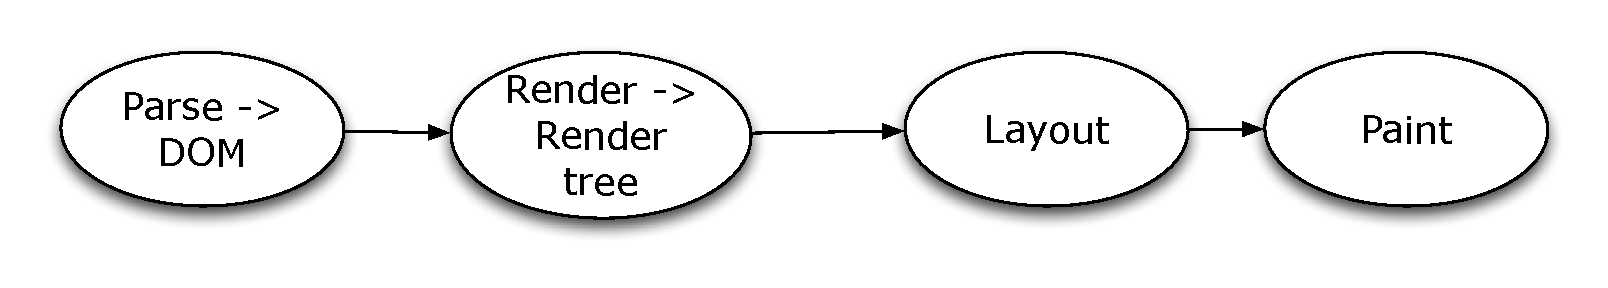
\includegraphics[width=11cm]
{rendering.eps}}
% Kommandoen \fbox tegner en ramme.
\end{center}
\caption{The rendering engine's responsibility}\label{fig:render}
\end{figure}

WebKit\cite{webkit} and Gecko\cite{gecko} are two popular rendering engines that implements the rendering process in figure \vref{fig:render}, however they do differ slightly in their internal behavior. WebKit is the engine that runs Chrome and Safari, while Gecko runs Firefox. In this section we limit the discussion to concern only these platforms, as they are built upon open source solutions and thus have available technical descriptions. The text that follows describes the process of rendering a complete HTML page. This usually happens when the client-browser requests a URL for an HTML page and the browser "refreshes" the page with the new content.

\paragraph{Parsing} 
The rendering of an HTML page starts when the networking layer is instructed to fetch a URL, say \textit{www.google.com}. Once the HTML page is fetched, the browser will immediately start fetching all external \textbf{links} that are contained inside it, from top to bottom. This could be links to CSS stylesheet pages, JavaScript pages, images, videos, etc. The rendering engine will continuously request chunks of HTML and CSS data from the networking layer, that it parses. An important feature of the HTML document's structure is that all the markup elements (tags) are nested in a hierarchical structure. Thus, when the HTML document is parsed, its tags are laid out in a tree structure.

Whenever the parser hits a script tag, it will first fetch the script if it is referencing an external file. Then, it will execute the script immediately. Unless the tag is marked "deferred" in which case the handling of the script will be postponed until the HTML parsing is done, the parser has to wait until the script is both fetched and executed. This is because the script might try to manipulate the HTML. To improve performance by avoiding the HTML parser to block while scripts are loaded, scripts can also be marked as "async" in which case the modern browser will generate a separate thread that fetches (if the script is not embedded in the HTML) and parses the script, while the main parser thread can continue and parse HTML. 
 
 The tree that is generated is called the \textbf{DOM tree}, where each tree element is named a DOM element. The DOM tree offers a programming interface (API) that can be used by JavaScript in order to manipulate the HTML. When the whole HTML page is completely parsed, the rendering engine will start executing the scripts that are marked "deferred". When these scripts are finished executing, the browser will generate a \textbf{DOMContentLoaded} event. Finally, when all the external resources are fetched and parsed, the browser will generate an event called the \textbf{load event}. The purpose of these events is that JavaScript execution can be set to execute, first once any of them is triggered.

\paragraph{Rendering}
While the DOM tree is being populated, the rendering engine will also start generating the \textbf{Render tree}. This is another tree that is a visual representation of the DOM tree, and in effect decides the style and order of how the DOM elements should be laid out. Every element in the Render tree has a reference to its DOM node, a style, and in addition they know how to layout and paint itself and its children. In effect each render element represents a visual rectangle on the screen. 

\paragraph{Layout and Painting}
In the layout process, each render element is given coordinate instructions for where on the screen it will be placed, and its size. The calculation is performed recursively from the root HTML node to the bottom.
The painting process does the actual work of painting the elements on the screen. It does so by iterating through the rendering tree and paints each component.
 
\subsection{JavaScript}
JavaScript is an interpreted programming language primarily built for manipulating Web pages. The language was developed at Netscape in 1995, during the time when Netscape and Microsoft were battling for the majority of browser users. The language itself was built in only 10 days, by Brendan Eich\cite{jsin10days}. He had instructions to develop a language that would look like Sun's Java, only simpler, interpreted and easy to integrate into Web pages, so that it would appeal to non-professional developers. Eich designed the language to follow much of the syntax from the C programming language, only simpler and with a much more dynamic memory management system. 

Despite a considerable amount of buggy features in the language and some compatibility issues between the different browsers, JavaScript quickly became a  popular language for the Web. Developers could easily create interactive behavior like changing color on a button when a mouse hovers over it, give the user feedback if the input in a textfield is wrong, etc. Much of its success was because of its simplicity; there was a low barrier to add JavaScript behavior into Web sites. Because there is no compilation process, and no "start function", only independent functions that can easily be written and ``tossed'' around in the document, unprofessional developers could quickly implement exciting and dynamic features \cite{jsHowGotHere}. On the other hand, for this reason, many professional developers would consider the language of being strictly for amateurs and not suitable for professional developers \cite{UnderstoodJs}.  Its strength was clearly for small sized applications, as browsers at the time were not able to execute large-scale JavaScript code. Also, considering that the JavaScript language at the time was very simple and limited, the development of large-scale JavaScript Web applications was simply not feasible. 
 
In an effort to improve the language features of JavaScript, and its browser incompatibilities, a standardization process of JavaScript was given to the European Computer Manufacturers Association (ECMA) in 1996. The language was actually renamed to ECMAScript, although most people still refer to it as JavaScript \cite{jshist}. Unfortunately, as the standardization was being developed, the browser inconsistencies, especially between Netscape and Internet Explorer continued to grow. Many JavaScript frameworks were built as workarounds to the inconsistencies, but most solutions weren't good enough. This led to alternative solutions for highly interactive and graphical client-side behavior such as Adobe Flash\cite{flash} or Microsoft's Silverlight\cite{silverlight}. 

An important part of JavaScript's history was with the rise of \textbf{AJAX} (Asynchronous JavaScript and XML) technologies\cite{ajax}, which gained much attention right around a century after JavaScript was first introduced. AJAX is an API that offers JavaScript functions that makes the browser asynchronously fetch data from the server without having to refresh the current Web page. Instead, the requested data would be used to alter the  page. This would result in a much more interactive user experience because the browser would neither block while waiting for the result, or re-render and paint the whole DOM tree upon successful complete. Since the introduction to AJAX, JavaScript has increasingly become a very popular language, and it has also brought the attention of professional developers. This has led to successful framework solutions like JQuery\cite{jquery} and Prototype\cite{prototype}, which simplifies the development of complex dynamic behavior and fixes browser incompatibilities, so that the Web developer doesn't have to write specialized code for each browser.

The increasing popularity of client-side application development with JavaScript has led to powerful JavaScript engines in modern browsers, making memory management and JavaScript interpretation highly effective. In September 2008, Google built the Chrome browser with its V8 JavaScript engine\cite{v8}, stating that low performance JavaScript implementations are no longer sufficient. Other browser vendors followed along, and today JavaScript performance is more superior than ever. Still, however, there are drawbacks with the language itself. Even though libraries like JQuery and Prototype simplifies the development of interactive and cross-platform Web pages, it is easy to end up with a big pile of tangled JavaScript event handlers and unstructured functions (often called spaghetti code\cite{spagetticode}). Most of the reason is that the language lacks features like classes, modules and namespaces, which makes it difficult to develop flexible and maintainable large-scale JavaScript applications. However, a lot of work has been done lately to implement quality frameworks that provide comprehensible syntactic sugaring for the language. These frameworks use some of the nice, and for many unknown concepts of the JavaScript language such as inheritance and closures to enable a highly flexible and structured development environment. All this has led to the possibilities of building large-scale JavaScript Web applications that runs primarily in the browser. Good examples are Google's Gmail\cite{mail}, and Maps\cite{maps}.

\paragraph{Node.js}\cite{node} is a Web application framework built for using JavaScript as the programming language. This is one of the first (and most popular) solutions for developing JavaScript Web applications on the server. It runs on Google's V8 JavaScript engine. A big advantage this framework has compared to other frameworks such as Rails or Spring, is that it is single-threaded and event-driven. This is a completely asynchronous programming environment that is centered around events, where clients subscribe to events and are notified when the events are triggered. This avoids the blocking scenario that might occur in regular synchronous systems. 


\subsection{Client-server Interaction Schemes}
There are multiple ways the browser can communicate with the Web server. In this thesis, we mainly adhere to two different ways. Synchronous client-initiated requests, and asynchronous client-initiated requests. These communication schemes all use HTTP, and are client-pull based. However there are other push-based alternatives such as Comet\cite{comet}, and WebSocket\cite{websocket}, where the client and server maintains an open connection, and the server can notify the client of changes.

\paragraph{Synchronous}
In a synchronous HTTP requests, the client-browser asks the server for data, in which the browser will wait for the server to respond. The request is normally trigged by the user clicking an anchor tag (hyperlink), or submits an HTML form. This would usually result in a new HTML page that is returned to the browser, in which the browser would  start a complete rendering process to build a new DOM tree, and paint it on the screen. A normal term for this is a page \textit{refresh}, or \textit{reload}.

\paragraph{Asynchronous}
In asynchronous HTTP requests, the client sends a request to the server, without the browser having to block while waiting for the result. Usually this happens with an AJAX request. When the result is received from the server, a browser event is triggered that is normally picked up by a JavaScript handler function. Typically the JavaScript handler alters the DOM tree with the new data received from the server.

One potential drawback with AJAX is that not all browsers support JavaScript. Examples are some smartphone devices or PDA devices.  Also, pages that are generated using AJAX are not automatically picked up by Web crawlers, because most Web crawlers do not access JavaScript code. This means that content generated by AJAX would normally not show up in public Web searches. However, in 2009, Google proposed a programming technique to make AJAX pages crawlable\cite{ajaxcrawl}. This is a somewhat complex technique, and can be tedious to implement in larger JavaScript applications.


\subsection{HTTP Sessions}
An HTTP-session is a semi-permanent communication dialogue that exists for two communicating entities (here, the client and the server). A session normally has a time-out value, such that when the time runs out, the session ends. The HTTP protocol is stateless in its nature, because every HTTP request is self-contained, and independent of every other request. Therefore, to be able to maintain state in an application, the client and server can incorporate a session protocol. The state information itself is data that has to be maintained between multiple pages in the application. Examples are shopping cart information in an e-commerce site, flight booking details, or authentication credentials. Imagine the user having to identify himself for each request that is sent to the server. This can be avoided if state information is persisted and being referenced in each request. 

There are a couple of ways to implement sessions:
\begin{itemize}
\item{} An object that is kept on the server . This object can be referenced in the client's cookie, or in the URL, if cookies are not supported. 
\item{} In the messages sent between the client and server, for example by populating the cookies, or keeping the data in the HTTP request and response body, or in the URLs. Clearly the size of the session data is very limited in this case.
\item{} In the browser's own storage system, thus maintaining sessions only on the client.
\end {itemize}

\subsection{Representational State Transfer}
Modern Web applications often follow a design pattern named Representational State Transfer, or simply REST \cite{armando2012}. This pattern states that all HTTP URL's must reference a particular resource on the backend, by using one of the HTTP request methods Get, Post, Put, or Delete (HTTP also supports additional request methods, but these are the most commonly used). This way, every URL offered by the Web application are self-contained in that it contains all the necessary information needed to satisfy a request. Resources are uniquely identified by a URI, and manipulated through the HTTP method interface. Applications that follow this pattern are named RESTful applications. A common use case for RESTful applications is to offer the self-contained URL's publicly as an API to clients other then just the application's own front-end, like other third party applications that wishes to use the applications REST services. Further, the REST pattern states that each REST request is stateless, hence adhering to the nature of HTTP which is stateless. That means, REST requests should not depend on an ongoing session in order to generate proper results.

\subsection{JSON}
JSON\cite{json} (JavaScript Object Notation) is a text based data format that is based on a subset of the JavaScript programming language. It is easy for both humans to read, and machines to parse, and has a similar syntax to many of the programming languages based on the C family of languages. The data structure fits well as a transmission format in Web applications, because it is both simple and light weight, easy to modify and is supported by many programming languages. The format itself is very simple, and the datatypes offered are limited to numbers, strings, arrays, booleans, and objects (being key-value pairs of the types just defined). An example of a JSON object representing a guitarist is showed below:
	\begin{lstlisting}
	{
		"username": "Paul ShredKing",
		"age":21,
		"country": "Norway",
		"guitars": 
		[
			"Gibson Les Paul",
			"Fender Stratocaster"
		]
	}
	\end{lstlisting}
The closest alternative to JSON is XML\cite{xml}, which is another transmission format often used on the Web, and especially with REST communication. However, its syntax is a bit more verbose, and requires more processing to manage because of its complex markup tags and syntax rules. On the other hand XML lets one add more restrictions to the data then with JSON.

\subsection{Business Logic and View Logic}
In Web applications, one often separates two very different programming concerns; the business logic and the view logic. The business logic (also called domain logic) typically represents:
\begin{enumerate}
\item{} The application's \textbf{domain}, often called business objects. They describe the application's core entities. Classical examples are Account, User, Purchase, Loan etc
\item{} The operations that can be performed on the business objects
\item{} Interactions between the business objects, and business rules that state the values that business objects are allowed to have
\end{enumerate}
The view logic (often called presentation logic) describes how the domain is visualized in the user interface. The view logic implements dynamic user interface behavior. It is often generated on the server, and depends on the application's current state. Typical Web 2.0 applications contain complex view logic.

Separation of business logic and view logic is considered best practice\cite{sepbiz} in order to let one concern change independently of the other, and to enhance a coherent codebase where separate concerns does not directly depend on each other\cite{bestprac}.



\subsection{HTML Template Rendering}
In dynamic Web pages, when an HTTP request comes in for a particular HTML page, the server has to prepare the HTML page with proper content based on the data received in the request. One way to generate dynamic HTML (that is, perform view logic) is to generate the HTML directly in code as Strings, and send the result back to the client. However this approach is messy, difficult to maintain, and the developer has to know the programming language that is creating the HTML strings. In other words, not a preferable solution for Web designers who only knows HTML. The preferable approach is a process called HTML template rendering. With HTML template rendering, a template system is organized as a set of \textbf{template files} (often called \textbf{views}), some domain and state data, and a rendering engine. The template files are implemented in a special template language. This is basically just HTML with additional syntax that refers to and can operate on data variables in the Web application. The operations supported are usually limited to simple loops and conditional expressions, just enough to facilitate the injection of dynamic data without confusing front-end designers. To generate a page, the rendering engine takes as input one or more template files, the data needed to populate the templates, and produces as output an HTML page. The necessary data is often fetched from the database or exists already in the server's memory. The resulting HTML page is sent back to the client. 

Recent JavaScript technologies have also enabled HTML rendering to happen in the client. The process is very similar. HTML template files can be sent to the client, which are ignored by the browser so the browser won't automatically paint them on the screen. Special JavaScript rendering engines that does the same job as the server-side rendering engine recently described can be accessed by JavaScript code in the browser. When some HTML template is to be rendered, the JavaScript rendering engine is called with an HTML template and a data object as input, and it returns an HTML page populated with the data content. The resulting HTML is typically appended to the DOM, or swapped with existing DOM elements. 

\subsection{Databases}
Databases, and especially relational databases have since the beginning of Web application history been the most popular form of storing persistent data\cite{armando2012}. Other alternatives have also been used such as flat-file storage (where the content is stored as plain text or binary data) or XML- or object databases. Much of the reason for the success of relational databases however, is that it provides \textbf{durability}, which in the context of data persistency means that once the data is stored, it is guaranteed to exist even if machines holding the data crashes. Also, a reason for the relational database's popularity is that it stores information in a structured format, which often fits the structured data formats that are manipulated by the Web applications. However, other types of databases that differs from the traditional SQL format has recently entered the marked. These are commonly referred to as NoSQL databases.

\subsubsection{ACID}
ACID is a popular term in the context of databases. It is a set of properties that guarantees reliability when it comes to transaction management. Database management systems often state that ACID guarantees are provided in their system, in order to promise a reliable database solution. Each property is defined below:
\paragraph{Atomicity} guarantees that either all the commands in a transaction completes, or non do.
\paragraph{Consistency} guarantees that all the data will always be in a consistent state according to pre-defined rules. A transaction brings the system to a new consistent state.
\paragraph{Isolation} guarantees that parallel transaction executions are always processed as if they happen serially, i.e no interference of any two parallel transactions. 
\paragraph{Durability} guarantees that committed transactions are safe, and lasts even during system errors or crashes. 

ACID guarantees are often provided by relational database management systems (RDBMS). However, NoSQL databases tend to have more relaxed relations to the principles, in favor for speed and simple replication abilities. 

\subsubsection{CRUD operations}
In Web application terminology, one often use the word CRUD to refer to the four essential  database operations; \textit{Create}, \textit{Read}, \textit{Update} and \textit{Delete}. These are the main operations performed by the Web application, on the data that needs to be persisted. When a CRUD operation is executed, it is the application's responsibility to convert the data into a format that fits the database's technology, and vice-versa. This process is called \textbf{marshalling}, or serializing. One example is when the application is to save a new object in the database. In this case, a \textit{Create} operation will be performed where the application will transform the object from whatever programming language syntax the object is currently described in, into a structure that fits the given database's syntax. The application will send this transformed (marshalled) object to the database, which is now able to parse the object and save it to its storage structure.   

\subsubsection{Relational databases}
Relational database management systems is a storage system based on a formalism known as the relational model. The formalism is based on structure and relationships, where the data entities are stored into \textbf{tables} that contain a set of \textbf{attributes} that describe the table. The tables can be related to each other to form groupings. RDBMS's stores a collection of tables, where each data entity is represented as a \textbf{row} in a specific table, and each column in a row represents an attribute for that entity. The most popular form of manipulating data in a RDBMS is SQL (Structured Query Language)\cite{sql}. This is a query language used to insert and manipulate data in a relational database. There are popular dialects of the language, generated by database vendors such as Oracle's SQL\cite{oracle}, Microsoft's MS SQL\cite{mssql}, MySQL\cite{mysql} and the open source PostgreSQL\cite{postgresql}.

\subsubsection{NoSQL}
NoSQL is a broad class of various database management systems who all have in common that they don't share the relational structure from normal SQL databases. The reason for its existence starts with the rise of Web 2.0 applications, when developers saw the need for simplifying replication of data, higher availability, and a new way to manipulate data that can avoid the need to perform tedious mappings between SQL strings and objects in any given programming language\cite{tedorm}. The main potential for NoSQL databases is to perform operations on massive amounts of data that is not structured or connected in complex relationships. Very often this applies to Web 2.0 applications, because much of the information in such applications can be gathered in coherent entities, thus avoiding the need for complex relationships and tedious operations to join them together. A typical example is users that has arrays of blog posts, and blog posts has arrays of comments, in which case all these fields are nested inside the user abstraction.

What's typical with NoSQL is that they are often customized to solve a particular type of application's persistency need. Therefore, there are many different classifications of NoSQL databases, which vary in the way they structure the data. An overview of the some commonly used NoSQL categories is summaries in the following list:
\begin{description}
  \item[Key/value store] \hfill \\
	Is a simple database store where data is identified by a key, and the data itself can be any datatypes usually supported by the implementing programming language. The structure is schema-less, meaning it doesn't provide complex structures with foreign key constraints. It is also highly efficient as the database is often implemented as a HashMap. One popular example is Redis\cite{redis}. This is an extremely fast key-value store that favors speed over durability. It also provides simple replication support, making it easy to distribute the database over multiple machines. Much of the reason for Redis' extremely high speed is because the data is typically being kept in memory, and only written to the database as a snapshot every once in a while. Other popular key/value stores are Riak\cite{riak} which favors scalability and fault tolerance, and Voldermort\cite{voldermort}, which favors simple distribution (data is automatically replicated). 
	
  \item[Document-oriented databases] \hfill \\
  Is a datastore that is based on documents that contain unstructured content. Documents are often separated into unstructured collections (can be viewed upon as SQL-tables), where unstructured here means that content in the same collection can have different structure. However there is some variation in the way the different database implementations choose to define the formats of the documents, but it can be assumed that each document encapsulates some logically associated data in a predefined format. An interesting property with these databases is that performance is often not the main goal, but rather programming satisfaction. As many of these are implemented in JavaScript and offers querying semantics and data structures based on JavaScript objects, it is really easy and flexible to perform database operations on them. Examples include CouchDB\cite{couch} and MongoDB\cite{mongo}.
  
  \item[Column-oriented databases] \hfill \\
  Is a database system where data is organized as columns, as opposed to row-oriented databases such as SQL based databases. In this scenario, every value that would usually be in a row gets its own instance in a column together with its belonging identifier (Id). As such, it is very efficient to perform range queries over a big amount of column data. Examples are Cassandra\cite{cassandra} and Google Big Table \cite{bigtable} (although these are not pure column-oriented, but rather a hybrid). 
\end{description}

\section{Summary}
We started this chapter by looking at how the World-Wide-Web began in the late 80's. In the beginning, Web sites were primarily a collection of static pages, but gradually turned into more dynamic pages where the content changes depending on attributes provided by the client. After this we saw that some of the technologies that are found on the Web today are outcomes of the browser wars that started in the mid-90's. This especially concerns the JavaScript programming language, which has resulted in many browser incompatibilities and a somewhat misunderstanding and unawareness of JavaScript's core language features and capabilities. However, major browser vendors, and Google especially, has acknowledged the advantage of having a unified language for the Web, something that has brought a lot of attention and improvements to the JavaScript programming language and its related technologies. This has now made JavaScript become a highly popular language for the Web, and developers have started building large-scale dynamic Web applications purely in JavaScript.

In the second part of this chapter, we looked into popular technologies that are commonly found in modern Web applications. Examples included AJAX, which offers an asynchronous client-server communication scheme, REST, which is a design pattern that states that Web resources should be manipulated exclusively through methods specified in the HTTP protocol (get, put, post, or delete), and NoSQL databases, which are databases that doesn't abide to the relational model, but instead specializes in speed and scalability through replication. We also looked at a specific type of modern Web applications, namely Web 2.0, which we saw were interactive Web apps with responsive and rich user interfaces, and social networking features.  

   
 % 20 sider
% Innf�ring i st�tte-omr�der etc for oppgaven (rettet mot oppgavens problemstilling)
						


%%%%%%%%%%%%%%%%%%%%%%%%%%%%%%

% NICE EXPLANATION TO USE SOMEWHERE

% The need for fast, complex, and responsive AJAX-powered Web applications demands replication of a lot of this logic on the client side, dramatically increasing the size and complexity of the code residing there. Eventually this has brought us to the point where we need MVC (or a similar architecture) implemented on the client side to better structure the code and make it easier to maintain and further extend during the application life-cycle.

%%%%%%%%%%%%%%%%%%%%%%%%%%%%%%

\chapter {Design Alternatives for Modern Web Applications}
\section{Introduction}
So far we have discussed the behavioral trends in modern Web applications and the technologies that runs them. We saw that modern Web applications are often very interactive with rich user interfaces, that looks and performs like native desktop applications with graphical user interfaces. In this chapter we look at popular ways these applications are built. This concerns the application's \textbf{architecture}, which is a concept that describes the application's structure, at different granularities. 

The traditional Web application has in the last decade followed a thin-client approach where all the logic happens on the back-end. In such architectures, HTML pages are dynamically generated on the server and handed to the browser every time the client issues an HTTP request. Lately however, there has been an increasing interest in moving much of the application's logic to the client, and abandoning the server-side page generation in favor for client-side page generation. This is called a thick-client architecture.\footnote{The thick-client architecture is not a new idea; thick-client architectures have been around for many years, where programs are sent from the server and executed on the client. Often this would be online games, calculators, or other user-interactive applications. However, these applications depend on a specific program that is compiled and executed on the client, in other words, not traditional Web pages that uses common browser-supported technologies.} Still however, a lot of applications follow the traditional approach, as many developers and application owners are skeptical to the thick-client model; this architecture implies heavy use of JavaScript, which has since its beginning had a lot of opposition, and people are still using old browsers that does not fully support JavaScript\cite{ie6use}.

The main purpose of this chapter is to outline the differences between, and popular ways to build traditional thin-client architectures, and innovative thick-client architectures. This also includes popular database solutions for persisting data in Web-apps. The first part of this chapter is divided into two main sections, one for each architecture. After this we will see how these concepts have been used in the prototypes built for this thesis. We will refer to the traditional approach as \textbf{Reference-model 1.0}, while the latter approach will be referred to as \textbf{Reference-model 2.0}. Thus, these two will be our reference models for software architectures that are aimed to build modern, interactive and scalable Web apps. 

\section{Reference-model 1.0}
Going back approximately 15 years, dynamic Web applications where often built with Common Gateway Interface (CGI) technologies\cite{cgi}. With CGI, a Web server accepts URLs that are delegated to an appropriate back-end program. A process is started on the server, and the CGI program executes the given request, which results in an HTML page that is sent back to the client. This solution however, was not very scalable considering each request would trigger a new process on the server. Gradually, as the Web got more users and the applications became more complex, new Web framework technologies came along. Examples are PHP\cite{php}, Java EE\cite{j2eeglance}, Ruby on Rails\cite{rails} and Microsoft's .NET\cite{popFrameworks}. For many years, developers have been building Web applications with these technologies, where all of the application's logic is executed on the server. This implies that the back-end implementation has many responsibilities, and the front-end is simply a thin-client that doesn't need to do much processing. This is only logical, as back-end implementations run on powerful Web servers, and client devices has up until recent years not been able to perform demanding processing jobs.
	
\subsection{The Three-Layered Architecture}		
A classical way of separating concerns in a Web application is to divide the whole system into three different software layers. There are some variations to how these layers are separated, but in this thesis, when we refer to a three-layered architecture, we follow the layering structure outlined by Brown et al\cite{brown}. This architecture separates the system into a presentation layer, domain logic layer, and a data source layer. The layers reside exclusively on the back-end of the application. The front-end has little responsibility in this architecture, as its only task is to display the result that is produced on the back-end. The layers are designed to be very loose-coupled. This is done by avoiding that a module in one layer depends on a concrete implementation in a lower layer. Instead, they depend on abstractions (interfaces) which can easily be swapped out. This principle is often referred to as the dependency inversion principle \cite{dipioc}. The abstractions are not hard-coded into the layers, but are "injected" through function arguments so that the same function can be called again if one wants to change the type of a dependency. The benefits from having individual implementation details encapsulated in different layers, is that it is very easy to modify one layer without harming another, and components can easily be reused. This facilitates a flexible and maintainable codebase\cite{flexible}.
		
\paragraph{The Presentation Layer} is the application's main entry point. Each URL offered by the application is mapped to a dedicated handler (often called a \textbf{controller}) in the presentation layer. In modern Web apps, the presentation layer is often implemented with the \textbf{Model-View-Controller} pattern\cite{mvc}. This is an architectural design pattern that organizes the structure of the layer. In this pattern, \textbf{controllers} handle HTTP requests from the client and simply delegates to a proper business operation in a lower layer. The result from the business function is returned in terms of \textbf{model} objects, which implement the \textbf{domain} of the application. When a business function returns the controller, it looks at the result to determine which \textbf{view} to return back to the end user. The view might be an HTML page, an HTML template file, or another data-format like XML or JSON. The latter two formats are most often used if the request is an AJAX request. If it is a template file, the view is sent to a rendering engine before the resulting HTML is returned to the client. Often, template files have references to other template files, in which case these will be merged together by the rendering engine. This facilitates decoupled view logic with fine-grained templates that can be reused.

Another architectural structure is the \textbf{Application controller pattern}\cite[p.379-386]{poea}. This separates how objects are to be presented in the app, from the app's business operations, by adding a new layer which is responsible for deciding which page to show in which order. This structure is nice if there is a lot of logic required to decide the page's ordering and navigation scheme. However, as the most common architectural pattern for the presentation layer is with the MVC pattern, we will continue the discussion with this pattern in mind. 

When a URL request comes in through the presentation layer, it might go through a number of \textbf{filters} before control is handed to the controller. Filters can have different objectives like authentication, marshalling of different Web formats into an object in the programming language that is used, error handling or HTML form validation. Also, the presentation layer would check the URL for a session identifier in the request's cookie, or the Url itself. The session identifier is referencing a session object that is already residing on the server's main memory, or in a database. The session object can also be used to store state information for the User, and to hold authentication details. After the request has passed the filters, the appropriate controller handler is called, which delegates control to a business function, typically in the domain logic layer. 


\paragraph{The Domain Logic Layer}, also called the business logic layer, or service layer, is responsible for executing the business operations that are supported in the Web application. These are the functions that makes up the core services of the application. Like in the presentation layer, the domain logic layer operates on the domain objects (i.e models). The business operations in the domain logic layer uses the domain objects by executing operations on them. Examples are calculating the total price for an order of books, registering a new friendship between two users, or searching for recommended movies for a currently logged in user. The domain logic layer sends and receives domain objects from the data source layer in order to persist them in a database. 

There are multiple ways of organizing how the business processes are implemented in the domain logic layer. A simple structure is by using the Transaction Script design pattern \cite{poea}. In this structure, each business operation is implemented in a single self-contained and independent procedure (script). Each procedure is mapped to an operation in the presentation layer, that takes input from the presentation layer, performs business logic (e.g data validation, calculations etc) and stores data in the database. This approach is very simple, as there is no domain abstraction and complex object-structure, just independent functions. However as applications get complex this pattern might lead to code duplication as different transactions might have common behavior. Another more common and object-oriented structure is to use the \textbf{Domain Model design pattern} \cite{poea} where business logic is encapsulated in domain objects. For example a BookOrder class would have functions for creating a book order given a list of books and a user id, fetching a book order given an order Id, updating a book order, and deleting a book order. In addition, the domain objects encapsulate the data attributes that represent the state of the object. The domain objects can have dependencies on each other, and call each others function in order to gain code reuse.
	
\paragraph{The data source layer} is responsible for communicating with other systems, such as databases, messaging systems, external Web services, the filesystem etc. Traditional Web architectures uses a relational database management system, which is the most popular solution for choosing how to persist the data in modern Web-apps\cite{dbpop}. Thus our Reference-model 1.0 will define that data is persisted in a relational database. The reason for its popularity is much due to the relational model, which brings a flexible and highly efficient query language (SQL). Most computer science courses on databases teach SQL, so developers tend to think data relationally. Also, data safety guarantees are provided with ACID, and the wide offerings of relational database management systems with its many development toolkits makes it a natural choice. Not to mention, the technology itself is many decades old and therefore brings years of experience and documented best-practices. 

The data source layer is responsible for marshalling domain objects into proper storage representation (also called database mapping), and vice-versa. For instance translating a SQL table into a Java object. The data source layer has to connect to the database, handle database transactions and close database connections. Usually this is handled by the Web application framework, so the data source layer only has to worry about how to perform operations on the database. As with the domain layer, there are two popular design patterns for structuring the data source layer. One is with the active record pattern \cite{poea}, in which case each domain object would know how to perform CRUD operations on themselves. Another approach is the data mapper pattern \cite{poea} where there is one separate class for each domain object, that performs marshalling of the given domain object, and is responsible for implementing CRUD operations on behalf of its domain object. The data mapper pattern separates the persistence code out of the domain objects, but adds more classes to the system. The active record pattern has a tendency to grow big in size, if the domain objects has to support a large amount of complex database operations. 
	
There are also frameworks that perform the marshalling, given some simple configuration of the domain objects. These are called object-relational mapping (ORM) tools. They often provide caching mechanisms to avoid using the database as much as possible, and they allow the programmer not to worry about marshalling at all. In many cases this could lead to less code in the data source layer. \cite{tedorm} Examples are Hibernate \cite{hibernate} for java, MyBatis\cite{mybatis} for Microsoft .NET and Java, and LINQ \cite{linq} for Microsoft's .NET. It is important to point out that even though these frameworks hide the complexity of object-relational mapping, it does have some pitfalls. Many developers argue that by using ORM-tools you loose the ability to exploit the full features of a database management system\cite[p. ~124]{ormlame}. This includes the ability to do customized database tuning, and take advantage of special data types that are supported by specific vendors. Plus, the fact that an ORM-tool does indeed hide the object-relational mapping code, makes it harder to debug, and also, there might be some performance overhead due to the complex code that is generated by the ORM framework.	
	
\subsection{The Front-End}
Up until now, we have been discussing the back-end implementation of a traditional Web app. The front-end consists of the set of HTML pages, CSS style sheets and JavaScript files that makes up the user interface of the application. User-navigation in traditional Web apps is often done through HTML forms or hyperlinks, which leads to a new page that is completely rendered on the browser (a page refresh). 

Also, in cases where a highly interactive event is to happen, a dedicated JavaScript event handler that is registered to listen to certain events will perform the action. This could be displaying a pop-up window or an animation effect on a mouse-hover event. The event handlers are registered with the browser when the HTML page is first rendered. In traditional Web apps, these handlers are often self-contained and independent JavaScript functions that has no structure or modularity. In most cases, this is because of some developer's relaxed relationship to the language; the JavaScript code is developed by adding function after function that merely serves to implement a new dynamic feature. This often leads to spaghetti code\cite{spagetticode}, in cases for applications that include a lot of interactive JavaScript behavior\cite{spagethi}.
				
\subsection{Platform Environment}
Another aspect of the classical three-layered architecture is application tiering.\footnote{Application layering is a term that divides the code into separate logical software layers. Application tiering on the other hand, is another logical separation often associated with where these "tiers" are physically deployed. For instance a three-tiered Web application could have its presentation tier on the Web server, the logical tier on a dedicated application server, and the persistence tier on a dedicated database server.} A Web application is often divided into three tiers; the presentation tier, the logic tier, and the persistence tier. 

The Web server hosts the presentation tier which communicates with client users through HTTP. The Web server listens on port 80, which is the port number used for HTTP. The HTTP request is forwarded directly to the appropriate code on an application server. The application that runs on the application server communicates with the persistence tier that is usually hosted on one or more database servers. In a bigger production environment, it is normal to distribute the tiers into separate physical server machines (called horizontal scaling). Each server is hosted on a separate machine in a so-called \textbf{shared nothing} manner, meaning the servers on each tier are independent so they don't have to communicate with each other. This makes it easy to add more servers on demand without any synchronization difficulties. Note that when the persistence tier is composed of a relational database management system, a shared-nothing architecture is difficult to implement, due to the nature of the relational model \cite{cloudmanagement}. This makes it difficult to do horizontal scaling with relational database systems. 

However, some SQL systems are particularly designed to scale vertically\cite{sqlscale}, and many large-scale Web 2.0 applications does successfully implement shared-nothing architectures backed by multiple distributed SQL databases. One example is the social-networking site Pinterest\cite{pinterest}. A report\cite{scalepint} outlined their platform environment, which among others include:
\begin{itemize}
\item{} 88 MySQL servers
\item{} 180 Web servers
\item{} 240 Application servers
\item{} 200 cache servers
\end{itemize}
				
\subsection{Examples of traditional Web architectures}
In this section we look at two examples of some common, traditional three-layered Web application architectures. The examples use Web application frameworks that is made for different programming languages, and promotes different architectural solutions. The purpose is to propose a set of popular Web architectures, that will be used as a base to determine the architecture we use to design the first prototype in this project. 
				
\paragraph{MVC with Ruby on Rails}. The Rails framework for Ruby has become a highly popular backend technology for Web applications, having many big commercial users. The framework is built around the MVC design pattern \cite{mvc}. In a Rails application, the controllers act as thin classes that receives a URL request, and  delegates business logic to the models. A model is a Ruby class that implements the Domain Model design pattern. The views consist of HTML template files, often written in a template language like HAML\cite{haml} or Mustache\cite{mustache}. These templates can reference data variables in a model class, and are rendered into HTML files on the server before they are sent to the client's browser. 

The data source layer in Rails is typically built with the Active Record design pattern. This works by letting the model objects implement CRUD operations for manipulating the database. This way, every model class contains business logic operations and the functions required to persist and manipulate the particular model in the database.

\paragraph{Front Controller with SpringMVC}
SpringMVC is a Web framework that wraps the Java Servlet API technology. The Java Servlet API is a set of classes that implements low-level protocols to communicate on the Web (e.g HTTP). For example, the Java Servlet API implements an interface called \textit{javax.servlet.http.HttpSession}, which provides session management. This session implementation puts an Id (called the JSESSIONID) in the User's HTTP cookie. This Id refers a particular HttpSession object that belongs to the User, and it is maintained by Spring on the server. 

Just like with Rails, SpringMVC is also built around the MVC pattern. However, the framework also applies an architectural pattern called the Front Controller pattern\cite{frontcont}. This pattern works by having one central servlet (the front controller) that receives all HTTP requests, and delegates control to a set of components that handle the request. This can be seen in figure \vref{fig:springmvc}.
	\begin{figure}
	\begin{center}
	\fbox{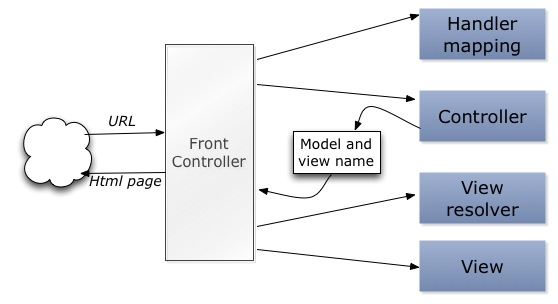
\includegraphics[width=10cm] {images/springmvc.eps}}
	% Kommandoen \fbox tegner en ramme.
	\end{center}
	\caption{A request flow with spring MVC}\label{fig:springmvc}
	\end{figure}
	
When a request comes in, the front controller will ask a \textbf{handler mapper} to get a reference to a specific controller based on information provided in the request URL. A controller is a SpringMVC component (related to the controller in the Model-View-Controller pattern) that is responsible for processing the actual requests. The handler mapper, is another Spring component that in addition to knowing what controller to issue based on a URL, performs pre- and post processing (i.e filtering) procedures, such as HTML form validation. When the handler mapper is finished pre-processing a URL request, it returns a reference to the right controller. The front controller then delegates the request to this controller. The controller typically just delegates to a business operation, and upon completion, it populates a model object with necessary data that is to be displayed in the view. The model object is a simple key-value data structure that lets the developer easily reference its data from the view file. The controller function also returns the name for the view that is to be rendered together with the model object. The view is a template file, often written in a template language such as JSP\cite{jsp} or Velocity\cite{velocity}. It is the view resolver that maps a logical view name (e.g "homePageView") to a physical view name (e.g "/WEB-INF/views/homePageView.JSP"). Finally the view and the model object is rendered to HTML and send back to the client. 
	
With Spring comes a great implementation of an inversion of control container (IOC)\cite {dipioc}. Inversion Of Control is a programming methodology where the concrete types of object references are not known at compile time, because the references are instantiated and populated  by an assembler at run time. This avoids having tight couplings between classes, and promotes a flexible codebase. The IOC container is a module that is responsible for creating objects, populate their references  to other objects, and manage their complete lifecycle. The container is fully configurable, which makes it easy to decide how the classes are instantiated. For example, objects can be configured to be lazily instantiated, meaning the object won't be instantiated until it is first referenced. Also, there are multiple ways Spring's IOC container can be configured to create objects. In Spring, this is referred to as the object's \textbf{scope}. Some common scope-alternative are:

\begin{itemize}
\item{} Request - one instance is created for each HTTP request
\item{} Session - one instance is created for each HTTP session
\item{} Singleton - only one instance of the given class is ever created.
\end{itemize}
			
A typical domain logic layer in a Spring application is built with the service layer pattern \cite{serviceLayer}. In the service layer pattern, the business logic is split into two. A service layer that exposes an API that encapsulates all the business operations, and the domain model which encapsulates the application's domain in separate classes that merely keeps data variables. The API, or service layer is categorized into logical abstractions called \textbf{services}, where each abstraction is hidden behind a facade \cite[p. ~158]{facade}. A facade is an interface that contains simple access methods to a more complex set of data structures, like complex business operations or database access methods.  Hence, each service encapsulates complex business operations and communicates with lower layer data source functions. The domain objects typically has no logical functions, only private data attributes with accessor methods, as opposed to the domain model design pattern. The service classes are also responsible for handling transaction management, so that if a transaction fails, the service classes know how to handle it. When performing database transactions, the service classes delegates to the data source layer which would know how to communicate with the database and perform object-relational mapping. This could be done by implementing a customized object-relation mapping scheme, for instance by implementing the data mapper pattern described earlier, or by using an ORM tool such as Hibernate or JPA\cite{jpa}. The latter case is similar to the active record pattern, often used in Ruby on Rails. Spring is one of the most popular frameworks for Java, as of 29th April 2013\cite{popFrameworks}.

\section{Reference-model 2.0}
The motivation for proposing a reference model for modern Web app architectures has its roots in an architectural shift that started around 2010, when browser's capabilities to execute JavaScript increased tremendously. This was by the time when Google launched its Chrome browser with the powerful V8 JavaScript engine, and the compelling browsers followed along with similar JavaScript capabilities. Also, The JavaScript language itself has started to get much more endorsement from the Web community with the standardization of ECMAScript, and Google's provenly working large-scale JavaScript applications like Gmail, Google Maps and also Node.js. This has led to many new experimental Web architectures that takes a distance from the thin-client model, and where application logic is gradually moving from the server and into the client. This means that the back-end is left being a simple and agnostic storage center for persisting the domain data in the application. Not only is this feasibly, but it's becoming increasingly popular. However, many developers have a skeptical relationship to JavaScript, partly because JavaScripts history of buggy features and browser incompatibility problems. Also, many developers are not aware of JavaScript's features like object-orientation including prototypal inheritance, and functional- and dynamic programming facilities, having closures and a dynamic typing system. Instead, they have acknowledged the fact that building large-scale JavaScript applications doesn't scale in terms of code maintainability; it often ended up as piles of spaghetti code\cite{spagethi}. This is an unfortunate misinterpretation. 

Together with this thick-client approach one has also seen a sudden interest in alternatives to the traditional relational database. With the increasing popularity of applications being deployed and run in the cloud, there is a need to be able to distribute an application's database over many servers. Now, because traditional SQL databases has showed not to replicate very easily\cite{cloudmanagement}, this issue, together with a need for a simpler programming interface against the database, has led to the many alternative NoSQL databases. 

In this section we propose an architectural approach where the application is moved to the client using JavaScript, and where data is persisted with NoSQL technologies.

\subsection{Front-end Frameworks}
An interesting aspect of modern Web application development is the evolution of JavaScript development environments. Not only has JavaScript been judged for being a language with many limitations, but it has also lacked proper frameworks and plugins for simplifying development of large-scale applications. However with the increasing interest for such JavaScript applications, a huge amount of frameworks and language variations have been built. This includes:
\begin{itemize}
\item{} Frameworks for structuring and organizing JavaScript code. \footnote{There is an project\cite{todo} on www.Github.com\cite{github} where developers are implementing the same Web application with different JavaScript frameworks to help developers choose a proper code organization framework for their Web apps.}
\item{} Programming languages that compile to JavaScript, to facilitate the development of large-scale JavaScript applications with a language that is more similar to traditional languages like Java or Ruby. Examples are Coffescript\cite{coffe} and Clojure script\cite{clojure}.
\item{} Frameworks for syntactic sugaring of the JavaScript language, useful mathematical operations, fixing browser compatibility issues, and simplifying working with the AJAX technology \cite{serrano2007ajax}. Popular examples are JQuery\cite{jquery}, Dojo\cite{dojo} and Backbone.js\cite{bakbone}.
\item{} Rendering engines for the front-end, built to produce HTML given a template file and data objects.
\end{itemize}

\subsection{Thick-Client Concepts}
Having the application moved to the client means that the one-to-one mappings between user interactions and controller handlers on the server are gone. Instead, these events are now picked up by JavaScript handlers on the front-end. The front-end has taken over many of the concerns that used to be implemented on the server. This includes: 
\begin{itemize}
\item{} Routing between pages
\item{} Render views into HTML
\item{} Sessions and state handling
\item{} Business logic operations
\item{} Deciding what to store in the database and when
\end{itemize}
 
Now, there might be other concerns that can be moved to the client as well, such as language translation of content and third-party API requests. However, I decided that this goes out of scope for this thesis. Also, there are variations in to what extend all of these responsibilities are performed on the client. For example, developers at Airbnb\cite{airbnb} found that they could benefit from letting the server be involved in routing between pages \cite{airbnbnode}. Also, Twitter \cite{twitter} found that letting the server participate in page rendering had good performance benefits\cite{timeToFirstTweet}. However, the main motivations for moving code to the client is because one might achieve:

\begin{itemize}
\item{} Better response-times, because tedious server requests can be avoided 
\item{} Better scalability, because less work has to be done on the server
\end{itemize} 
 
\subsubsection{Moving the Application to the Browser}
In Reference-model 2.0, the application relies on the front-end, and is completely written in JavaScript, or a language that is compiled to JavaScript such as CoffeScript, or ClojureScript. The JavaScript code can either be sent to the client all at once when the Web application is first accessed, or parts can be lazily fetched when needed. This requires the source code to be split into separate code files so they can be sent individually from the server. This might be a performance benefit in case the whole JavaScript codebase is very big. A pitfall however might be that very many small JavaScript files would be required and sent simultaneously, in effect potentially causing tedious transmission times. In some cases the TCP connection overhead might be a performance bottleneck because the browser usually creates a new TCP connection every time the browser requests something from the server. 

	
\subsubsection{Single-page Web Application Architecture}
One essential advantage with the thick-client architecture is that server requests might be limited. In the traditional approach, each user interaction with the page leads to a server request that result in a new page, and the browser has to reload the whole page. This causes a disruption in the user experience. With the modern approach, the request goes straight to JavaScript event handlers. This way, the client stays on the same page during the whole session, requiring no new page reloads. If for instance a link in the navigation bar that leads to a different page in the application is requested, everything is done in the browser by manipulating the DOM tree so that the new page is displayed. This could lead to a much more fluid user experience, because server requests can be avoided, and the browser does not have to reload the entire page. This principle is commonly referred to as a Single-page app\cite{spa-man}.

If the front-end needs to synchronize data with the database it will send an asynchronous data request to the server with AJAX. This could for instance be to save some data, or get some new data that needs to be displayed on the page. The client can also store data in the browser's memory, such that the more domain objects stored in the browser's JavaScript memory heap, the less requests has to be sent to the server. Depending on the application, write, update and delete operations will always sooner or later have to lead to a server request, so that every user has an up-to-date view of the data. In applications that require all updated data to be available as close to real-time as possible, the data has to be directly written to the database, in effect work as a write-through cache. In applications where this requirement is more relaxed, the front-end can choose to perform persistency at a later and more appropriate time. For Web 2.0 applications, the former is often wanted, because users usually want to see the latest updated data at all times. 
		
\subsection{The Simplified Back-end}
The responsibility of the backend is mainly to manage the database. It's interface is still exposed as controller handlers, however these are not customized for particular HTML form requests or hyperlinks that leads to a new HTML page. Instead, the backend exposes an \textbf{API} for manipulating with the application's domain in the database. This API contains a set of public functions where each function is identified by a specific URL. Each URL refers to a domain entity in the application, and an operation that the server is to perform on the domain object. Note that this operation is usually not a complex business operation, but merely a single database operation. The operations offered by the backend API are commonly expressed using merely HTTP methods. Hence, the server API is a RESTfull service that adheres to the principles in the REST design pattern. Now, instead of creating and returning a complete HTML page upon each client request, the server would return a more fine-grained data object represented in a uniform data format such as XML or JSON. This is a much more general-purpose solution, because external clients like mobile applications and other third party applications can now use the service offered by the application, and so choose how to use and display the returned data.\footnote{A typical service-oriented architecture}

In respect to Reference-model 2.0, the back-end can be implemented using basically every server-side Web application framework, considering the responsibility of the back-end is so very simple. Popular choices are among others Ruby on Rails, SpringMVC and Node.js\cite{popFrameworks}.

\begin{table}
	\centering
	\begin{tabularx}
	{\linewidth}{ |X|X|X| }
	    \hline
	    \textbf{Method} & \textbf{URL}  & \textbf{Description} \\ \hline
	    Get & www.shredhub.com/ shredder/1234 & Get shredder with id 1234 \\ \hline
	    Post & www.shredhub.com/ shredder/ ?name=Jude Swayer & Add shredder with name Jude Swayer  \\ \hline
	    Put & www.shredhub.com/ shredder/ 1234?country=Sweden & Update shredder with id = 1234 set country = Sweden \\ \hline
	    Delete & www.shredhub.com/ shredder/1234 & Delete shredder with id 1234 \\ \hline
	    \end{tabularx}
	    \caption{A simple REST API}
	    \label{table:urls}
	   \end{table}
	   
\subsubsection{REST API's and JSON}
The thick-client model avoids letting the user communicate synchronously with the server. Instead, the JavaScript application that runs in the browser is responsible for knowing when it needs to communicate with the server. This would be whenever some domain objects that are not already in the browser's heap are requested, or some domain object must be persisted to the database. The requests to the server are exclusively done through the RESTful API. This means that all domain objects that are to be offered by the server, must be accessed through one of the HTTP methods \textit{Get, Post, Put, or Delete}. An example of a RESTful API that offers functions for persisting a Shredder object is showed in table \ref{table:urls}. A shredder is a guitarist in the Web app prototype that has been created in this thesis.
	    
	The server would respond with the domain objects in JSON format, instead of a complete HTML file. This way, it is up to the client how to visualize the result-data. Also, the API is very consistent, because it adheres to a common interaction scheme, namely the HTTP request methods Get, Post Put, and Delete. This creates a familiar and easy-to-understand server API. This programming interface works really well with the thick-client model, because the client tier can be completely responsible for maintaining the application's state, and thus the server can be stateless.
	
Modern REST API's very often use JSON as the transmission format, because it fits well into the programming model both on the front-end and back-end, because considering that the front-end code is implemented in JavaScript, and JSON is part of the JavaScript language, it is very appropriate to use JSON as a transmission format because no marshalling has to be done on the client. This might also apply on the back-end: Some NoSQL technologies stores JSON-like objects, in which case no marshalling would be needed if the programming language used supports JSON.
	
\subsection{Modular JavaScript}
A modular codebase is made up of highly decoupled, encapsulated pieces of coherent features that are implemented in separate modules. A codebase that consists of loosely coupled modules, facilities a flexible and maintainable system, because the codebase contains less dependencies\cite{flexible}. This makes it easier to change one part of the system without harming any other.  

The JavaScript programming language does not have module features built into the language. This means that it is up to the developers themselves to develop some sort of module framework. Various design patterns have been proposed to establish standard ways of developing modules, like the module and sandbox pattern \cite{jspatterns}. These are patterns that gathers related code into coherent modules, fairly similar to classes in traditional object-oriented languages. A lot of work has been done to provide open solutions for JavaScript developers to build modular JavaScript code in the browser. A common solution is Asynchronous Module Definition (AMD)\cite{amd}, which is an interface proposal for how to create modules in JavaScript. Having the JavaScript code separated into modules means that these modules can be split into separate source files and have references to each other. That is what facilitates the lazy loading of JavaScript files previously mentioned.
AMD makes it possible for the modules to depend on each other, and also on HTML templates, so that whenever a JavaScript module is fetched from the server, the HTML template will be fetched as well, and will be available as a text string inside the JavaScript module.
	
The AMD principle was also made to have a better alternative to loading scripts then the traditional group of \textit{<script>} tags embedded in HTML files. The problem with this approach is that it doesn't say anything about the loading order, meaning if any of the scripts depend on each other, there is no guarantee they will be fetched in the right order. AMD brings an API that defines all the dependencies for the modules. As such, when a module is needed, all its dependencies are first loaded asynchronously, and when they're all received from the server (or some other external source), the dependencies are made accessible inside the module. The AMD API comes with two functions: \textit{require()} and \textit{define()}. \textit{Define()} is used to encapsulate a JavaScript module, and make it globally accessible, while at the same time define the other modules it depends on. The \textit{require()} is used to asynchronously load modules into a function, in which the function will not be called until all the modules are loaded and ready to be used inside the function.


\subsection{Client-side Page Rendering}
What is special with Reference-model 2.0 is that rendering HTML is no longer a matter of rendering a complete HTML page, but rather render the parts of the HTML page that need to change, and render this immediately without consulting the server. One approach is to write blocks of HTML with JavaScript strings, and write this to the DOM when a page needs to change. However, this is not very clean, or maintainable, especially when building large applications.

Using HTML templates are preferable as these can be reused, are easy to read and can be cached in the browser. Whenever the HTML need to change, a JavaScript rendering engine will be consulted which performs the rendering. The result is either appended to the DOM, or swapped with current DOM elements.

As previously mentioned, the AMD model makes is possible to have JavaScript modules that depend on HTML template files. This facilitates a nice programming model, because if the HTML pages are also separated into small independent templates, then these templates can be stitched together to form complete HTML pages. As such, HTML templates can be reused, removed or swapped out from the current HTML page by the JavaScript renderer. This enables a highly flexible way of altering contents of the HTML page, and efficiently altering large parts of HTML without consulting the server.
		
\subsection{Client State and Navigation Handling}
Another part of Reference-model 2.0 is how the state is being kept between requests. The major goal of Reference-model 2.0 is to move much of the application logic from the server to the client. Thus, being able to keep the state client side is of high priority. In Reference-model 2.0, we propose an alternative solution to this by using HTML 5's Web Storage\cite{webstorage}. The HTML 5 Web storage is a standardization made by W3C that offers a way to store data in the browser between page requests. It is supported in all modern browsers. HTML 5 Web storage contains two storage containers: \textbf{localStorage} and \textbf{sessionStorage}. The difference is that local storage is being persisted even when the browser is closed, and it has no expiration date. The session storage is only kept in the browsers memory until the session is over, which means either if the user closes the tab or the browser. The Web storage enables developers to store lots of more data than what it supported with cookies. As an example, Internet Explorer 8 allows for sessionStorage up to 10 mega bytes, while a cookie is generally limited to 4 kilo bytes. The sessionStorage consists of a key-value data structure that is accessed by a simple JavaScript API.
	
A session implementation can be built by letting a JavaScript object be created when the Web application is first accessed by the client user. The object is populated with user data, and so each time the client tier changes state or receives some state information from the server, it can be persisted in the session object. Thus the server does not have to maintain a session object in memory for each user that is currently logged in to the Web application.

Navigation is done without consulting the server, meaning all User interactions that would normally result in a new page is now picked up by a dedicated JavaScript component. This component is often called a \textbf{router}. The router's job is to ensure a new page will be rendered in the browser (typically by delegating to a proper view-logic implementation), and change the browser's URL to match the new state.\footnote{Changing the browser's URL recently became much simpler with the HTML5 browser history API\cite{html5history}, which enables developers to change the URL with JavaScript.}

\subsection{Alternative Front-end Design Patterns}
There are many ways in which to structure the JavaScript code that runs in the browser. As we did for Reference-model 1.0, we will look at some popular architectural design patterns for structuring front-end code. 
\begin{itemize}
\item{} MVC/MV*: Traditional Web-apps often implements the MVC pattern. In thick-client architectures, this pattern is often used, however with some variations.  Models represent the domain data and communicates with a back-end API, while views contain logic that handles the user interface (\textbf{view logic}). In Reference-model 1.0, view logic was done both in JavaScript handlers on the front-end, and controllers and HTML templates on the back-end. Controllers handle routing between views and models. However, MVC-style controllers in server-centric applications doesn't always transfer directly to the thick client architecture. Controller behavior is often implemented in both views, and the router. Therefore, a popular way to define a thick-client's architectural pattern is simply MV*, meaning models-views- and something else that's up to the developer. 

\item{} MVP: Is a pattern that decouples the views from models by introducing a mediator called the presenter. In this pattern, the view's responsibilities are merely thin containing little to no logic, all of which is done by the presenter. The presenter's responsibility is to handle all presentation logic and routing, and communicate with a persistency layer on behalf of the models. The pattern is mostly used in cases with complex views and many different user interactions, such that handling logic and routing can be separated and reused as much as possible in the presenters.
\item{} MVVM: Is a pattern that adds an abstraction called the view-model. Its responsibility is to turn models into their user interface representation, and delegate commands from views to models. Thus the views don't have to worry about how the models should look like, or how to delegate business logic. The pattern is also suitable when models must have many different view representations.
\end{itemize}

\section{The Solutions Chosen}
The two reference models just described are popular approaches to how developers design and implement modern, interactive Web apps. In this thesis, the goal is to compare these two approaches, in order to identify their strengths and weaknesses.  Therefore, the main concepts from these reference models are applied in two different software architectures for a prototypical Web app. The first solution is called \textbf{Architecture 1.0}, while the latter is called \textbf{Architecture 2.0}. 

Architecture 1.0 is a thin-client application, where the application relies on the back-end. The back-end is built as a three-layered architecture. This means that all the view logic happens in the presentation layer on the server (and some is made with JavaScript on the front-end), business logic operations happens in the domain logic layer, state is being kept on the server using HTTP sessions, and the front-end tier is tightly coupled to the server such that each HTML form or link has a corresponding handler on the server which serves to generate a new HTML page given the result of the request. The back-end is built with Spring MVC, and is therefore a Java Web app. It uses a SQL database to persist data, and does not use any ORM tool to perform database mapping. 

Architecture 2.0 is a thick-client architecture where the application resides on the front-end. State management, controller handling and business logic all happens in the browser, which is built purely with JavaScript. The front-end uses the MV* pattern, where models are active record objects that uses the back-end only as a simple data repository. The back-end is offering its services through a Rest API, which is built with Node.js. The Rest API manipulates the database, which is a MongoDB database. 
			
\begin{table}
\centering
	\begin{tabularx}
	{\linewidth}{ |X|X | }
	    \hline
	    \textbf{Reference-model 1.0} & \textbf{Reference-model 2.0} \\ \hline
	    Server-side page rendering & Client-side page rendering \\ \hline
	    Application logic is on the server (thin-client) & Application logic is in the browser (thick-client)  \\ \hline
	    Session state stored on server & Session state stored in browser \\ \hline
	    HTML Form-based interaction with complete HTML pages returned to the browser & RESTfull AJAX requests for JSON objects and fine-grained HTML templates used to alter the DOM \\ \hline
	    SQL database & NoSQL database \\ \hline
	    \end{tabularx}
    	    \caption{Comparison of the two reference models}
	    \label{table:compare}
    \end{table}

		
\section{Summary} 
In this chapter we have discussed two very different Web architectures. A short comparison of these two is given in table \ref{table:compare}. The table sums up the major differences between the two architectures, where each row concerns similar architectural issues. 

Reference-model 1.0 had a thin-client model with all the business logic performed on the server. The server's job was to perform the business operations, execute database operations and create create HTML pages. This is a common solution to building Web apps. Reference-model 2.0 is a thick-client architecture where most of the logic is performed in the client's browser, primarily using the server for database manipulation. A flexible thick-client codebase can be achieved by using popular architectural patterns such as MV* and MVP, and by using syntactical sugaring front-end frameworks. The RESTfull architecture, together with asynchronous HTML/JavaScript loading might result in less data sent between the client and server. 

Reference-model 1.0 uses a traditional SQL database to persist data, while Reference-model 2.0 uses NoSQL databases. The latter approach is more suited for replication, and might provide a simpler programmer interface. SQL, however, is the most popular persistency solution for Web applications. At the end of the chapter we stated that the two reference models are used as a base for designing and implementing the two architectures that have been built for this thesis. 
 % 15 sider
% Hovedvalg og vurdering av disse.
% Etter veiledning med Arne, skal dette kapittelet dr�fte dagens l�sninger av begge arkitekturer.
% S� skal det naturlig komme inn i hvilken arkitektur jeg har valgt, samt vurdering av disse.

\part{The project} % 40 sider
% 15 sider overordnet diskusjon + 25 sider finkornet diskusjon
% Hovedlinjer og viktige detaljer i programmer.
% Se p� alternativer og utvidelser     
\section{Overview}
This part covers the project that has been developed for this thesis. It contains a Web application that has been built twice with two completely different architectural approaches. The main goal in this thesis is to find a superior software architecture for a typical Web 2.0 application, by comparing a traditional architectural approach with a modern and innovative approach. In order to evaluate these two architectures, the writer of this thesis has invented a Web app that represents a traditional Web 2.0 application. This Web app contains the most commonly seen features of a traditional web 2.0 application. This includes:
\begin{itemize}
\item{} Social networking interactions:
	\begin{itemize}
		\item{} Have a user-profile that is publicly visible to other users
		\item{} Connect to other users, for example in a friendship relationship
		\item{} Creating blogs and upload posts to it 
		\item{} Ability to comment and rate blog posts
	\end{itemize}
\item{} Interactive behavior with rich user interfaces
\item{} Large amounts of persisted data (this mainly because the app-users themselves create the information content)
\end{itemize}

The first architecture that was built conforms to a traditional approach, and the second conforms to a modern approach. 

The rest of this part is separated into three chapters: In the first chapter we will look at the Web app itself, seen from the end-user's perspective. A description of the Web app's user behavior and requirements is necessary in order to understand the solutions that was taken when designing the software architecture for the app. The Web app is named Shredhub. In the last two chapters, we will have a detailed look at the two ways the app was built. The architecture outlined in the second chapter, is named Architecture 1.0, and is adheres to the principles from \textit{reference-model 1.0}. The final chapter discusses the architectural details in Architecture 2.0, which is based on \textit{reference-model 2.0}. For the record, during the discussion we will use the term \textit{User} to refer to the currently logged in user.
\chapter{Shredhub, a Web 2.0 Application}
This part of the thesis covers the prototype that has been designed and built in order to compare the two architectural approaches. The Web app has been built twice from the ground-up, using two completely different architectures. The Web app contains common features found in traditional Web 2.0 applications. This includes:
\begin{itemize}
\item{} Social networking interactions:
	\begin{itemize}
		\item{} Users have their own profile account that is visible to other users
		\item{} Users connect to each other
		\item{} Users can creat blogs posts, and rate and comment on other posts
		\end{itemize}
\item{} Interactive behavior with rich user interfaces
\item{} Large amounts of persisted, user-generated data
\end{itemize}

The rest of this part is separated into three chapters: In this chapter we look at the Web app itself, seen from the end-user's perspective. In the last two chapters, we will have a detailed look at the two ways the app was built. For the record, during the discussion we will use the term \textit{User} to refer to a currently logged in user.
	
\section {The Concept}
Shredhub, is a social Web application for musicians, aimed primarily for guitarists. The application enables users to share their skills and musical passion in a social and competing manner. Through a modern and interactive user interface, the users are able to post videos of themselves playing a short tune. Everyone can watch, comment and give a numbered rating to the videos, so that the creator can achieve experience points and become highly ranked on this social platform. 
		
Now, it is important to acknowledge the fact that this application is primarily for guitarists, which does imply a slightly small user group. A better solution would be to implement a system that supports more kinds of musicians, for instance drummers, piano players, saxophone players etc. Therefore, a better solution could be to let the users pick their preferred instrument before they access the application's main page. From there on they would only be able to participate with the kind of musicians the user picked at startup. However, because I have only had a certain amount of time to implement this application, extending the application unfortunately goes out of project scope. Therefore I content myself with only supporting guitar players in this project. 
		
\section {User Functionality}
There are many terms and concepts used on Shredhub. Here is a general overview:
\begin{itemize}
\item{} A \textbf{Shredder} is a user on shredhub. The shredder has a profile that includes (among other things): profile-image, list of guitars, list of equipment, home-country, experience points etc
\item{} \textbf{Experience points} is a rating of how skilled a Shredder is. This rating changes when someone rates a Shred the Shredder has uploaded
\item{} A \textbf{Shred} is a video of a Shredder playing a short tune. The Shred has a set of tags \footnote{Tags is a widely adopted term in the world of Web 2.0\cite{web20book}; many web 2.0 applications use tags to classify things like blogs and images} that categorizes the video. Other Shredders can rate and comment the Shred. Also, Shredders can remove a comment they made.
\item{} \textbf{Shredders} connect to each other in fan-relationships, meaning a Shredder A can be a fan of Shredder B, such that Shredder B is a fanee of Shredder A. 
\item{} Two Shredders can \textbf{Battle} each other in a Shred-battle. This is a turn-based game where Shredders upload Battle-Shred videos in a specific battle-category. Others can rate the Battle-Shred videos, such that the purpose is to have a highest summed up rating. 
\end{itemize}
		
\section{Pages and User Stories}
Given below is the set of pages and user stories in Shredhub. Each page is outlined together with its URL, and a user story that is found on the page. Notice that the URLs are not real in this discussion, they are just fictive examples.
\begin{description}
		
\item[The front page, www.shredhub.com] \hfill \\
The User is first met with a front page as seen in figure \vref{fig:frontpage}. Here the User can either register as a new Shredder, or log in with a username and password. The User will not be able to access any of the other services in the app before he is logged in. The page also displays a set of the current most popular Shred videos.
\begin{figure}
 \begin{center}
\fbox{\includegraphics[width=\textwidth] {images/frontpage.png}}
% Kommandoen \fbox tegner en ramme.
\end{center}
\caption{The front page at Shredhub}\label{fig:frontpage}
\end{figure}

\item [The shred pool, www.shredhub.com/theshredpool] \hfill \\
This is the first page the Shredder meets when he logs in. It is the ``main-page'' on Shredhub, which contains multiple rows of Shreds made by other Shredders. The page contains the following rows of Shreds:
\begin{enumerate}
\item{} The latest Shreds
\item{} Shred-news:
	\begin{enumerate}
		\item{} Newest Shreds made by fanees
		\item{} Newest Battle-Shreds by fanees
		\item{} Newly created Battles by fanees
		\item{} New recommended Shredders to connect to
	\end{enumerate}
\item{} Shreds with particular high rating
\item{} Shreds from Shredders that might be of interest
\item{} Shreds based on tags the User enters
\end{enumerate}

Every row contains a collection of 3-5 Shreds, except the final row which contains 20 Shreds. The User can click the next button in a row, which results in a new row of Shreds. The Shred-news section is a set of Shreds and Shredders especially picked out to fit the User's profile, that is, new content made by his fanees, and recommendations for new Shredders. The Shredpool is showed in figures \vref{fig:theshredpool1} and \vref{fig:theshredpool2}

The shredder can also create and upload a new Shred by clicking "Upload shred". If the Shredder clicks on a particular Shred in any of the rows, a new window pops up displaying the Shred video.
		
\begin{figure}
  \begin{center}
\fbox{\includegraphics[width=\textwidth] {images/shredpool1.png}}
% Kommandoen \fbox tegner en ramme.
\end{center}
\caption{The Shredpool (top)}\label{fig:theshredpool1}
\end{figure}

\begin{figure}
  \begin{center}
\fbox{\includegraphics[width=\textwidth] {images/shredpool2.png}}
% Kommandoen \fbox tegner en ramme.
\end{center}
\caption{The Shredpool (bottom)}\label{fig:theshredpool2}
\end{figure}

\item [Shredders, www.shredhub.com/shredders] \hfill \\
This is an overview of all the the Shredders that are using the app. Considering that the amount of Shredders on the page might be very big, the list is paginated, meaning a fixed number (20 in this case) is displayed at a time, and the Shredder can click next to iterate to the next page of Shredders. Shredders can also search for other Shredders by name. The purpose of this page is to encourage Shredders to meet new Shredders so that their fan graphs can be extended. The User can click on a Shredder to access his public profile page. The shredders page can seen in figure \vref {fig:shredders}. \begin{figure}
 \begin{center}
\fbox{\includegraphics[width=\textwidth] {images/shredders.png}}
% Kommandoen \fbox tegner en ramme.
\end{center}
\caption{The list of Shredders}\label{fig:shredders}
\end{figure}
		
\item [Shredder, www.shredhub.com/shredder/<id>] \hfill \\
This is a page that displays the details for a given Shredder, that has the unique id found in the URL. A list of Shreds that the current shredder has published is displayed in a list view, together with a list of his fanees. The User may choose to challenge this Shredder for a battle, or become a fan of the Shredder. The page is customized to show the relationship the User has with this Shredder. This might be that they already are in a battle, or if a battle request is sent to this Shredder, if they are fans of each other already, and other similar relationships. The page can be seen in figure \vref{fig:shredder}.

\begin{figure}
  \begin{center}
\fbox{\includegraphics[width=\textwidth] {images/shredder.png}}
% Kommandoen \fbox tegner en ramme.
\end{center}
\caption{A Shredder's profile page}\label{fig:shredder}
\end{figure}
		
\item [Battle, www.shredhub.com/battle/<id>] \hfill \\
This page displays a battle between two Shredders. If the currently logged in user is one of the battlers, the User is able to upload a Shred for the battle. In a battle I distinguish between the battler who initiates the battle, and the battlee, being the one who is challenged. I have not added an image of a battle, because it won't be discussed in much detail in this thesis.

\item[Shred] \hfill \\
A pop-up window displays a particular Shred made by a Shredder. Users can add a rating to the Shred, and add comments for it. The Shred can be accessed from multiple different pages in the app. An example image is given in figure \vref{fig:shred}.
\begin{figure}
  \begin{center}
\fbox{\includegraphics[width=\textwidth] {images/shred.png}}
% Kommandoen \fbox tegner en ramme.
\end{center}
\caption{A pop-up window displaying a Shred}\label{fig:shred}
\end{figure}

\item[Upload a Shred] \hfill \\
For uploading Shreds, a simple pop-up window is displayed so the User can add a Video, a description, and a set of tags. This window can only be accessed inside the Shredpool. This can be seen in figure \vref{fig:addshred}

\begin{figure}
  \begin{center}
\fbox{\includegraphics[width=14cm] {images/addshred.png}}
% Kommandoen \fbox tegner en ramme.
\end{center}
\caption{A pop-up that lets the User add a new Shred}\label{fig:addshred}
\end{figure}

\end{description}
		
 % 3
\chapter{Architecture 1.0}
%Lines:
%	177 pom
%+	3859 api java
%+	1937
%+	305
%+	1668
%+	110
%+	426
%+	262 pom
%+	1159 jsp java
%+	2633
%+	265 xml
%+	116
%+	47
%+	2903
%=	15867

	
\section{Introduction}
In this chapter we will look at the architectural details of Architecture 1.0, which is an implementation of Shredhub that conforms to \textit{Reference-model 1.0}. The application is written in Java, and uses the SpringMVC framework. I could have chosen to use another technology like Ruby on Rails, Sinatra for Ruby or Microsoft's .net, considering these are all very popular Web application environments. However, because I happen to know the Java programming language very well, choosing a Java-based Web is preferable. Although there are other Java-based Web frameworks in addition to Spring, Spring was chosen because it is very easy to set up, it provides a wide collection of plugin extensions, it implements lower layer protocols like Http communication in a highly efficient manner, and most importantly, for the relevance of this thesis, it is one of the most popular Java-based Web frameworks.  

The application runs on Apache Tomcat, which serves as both a Web server, and an application server. The database is implemented with PostgreSQL. It runs on a database server which for simplicity is deployed on the same physical machine as Tomcat. Here I could also have chosen a different database technology, for instance MySQL or Oracle SQL. However, I chose PostgreSQL because I have experience with the technology, it also has a lot of good and available documentation, and it is a very popular database choice for modern Web applications. \cite{popularDB}


\section{Architectural Overview}
%\begin{wrapfigure}{r}{0.5\textwidth}
%  \begin{center}
 %   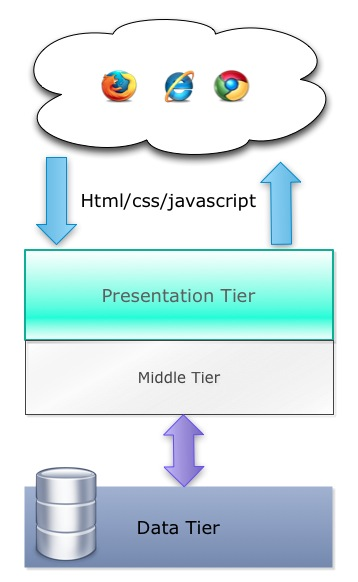
\includegraphics[width=0.48\textwidth]{images/architecture1.jpg}
 % \end{center}
 % \caption{Overal architecture 1.0}  \label{fig:architecture1}
%\end{wrapfigure}
%% FORTSETT
Architecture 1.0 is a backend-oriented Web app. All of the application's logic happens in a Web application that runs on an application server. In respect to \textit{Reference-model 1.0}, the application is separated into three software layers with different responsibilities; a presentation layer, a domain logic layer, and a data source layer. I have chosen this separation of concerns in order to facilitate application maintainability and flexibility. I could have chosen to implement everything in two, or even one layer, but this would resolve in classes having very many responsibilities, and possibly lots of code duplication. The layers cooperates by delegating responsibility. This means that the presentation layer implements client-server specific concerns, and delegates business logic specific operations to the domain logic layer. This layer implements business logic, and delegates to the datasource layer whenever it needs to address the database or some other data resource. The results from the operations done in the datasource layer bubbles up the layer stack all the way back to the presentation layer.

The Web app depends heavily on Http sessions to maintain user-state. When a user enters www.Shredhub.com, SpringMVC generates an object (called the HttpSession object) who's lifetime lasts throughout the user's session with the app. This object is used as a container for storing state information.

The application's front-end consists of a set of HTML pages that we will refer to as \textbf{Views}. The views are implemented with the JSP temple language technology, and are turned into HTML pages with the template view pattern. The client user primarily communicates with the app through three different interaction schemes: 
\begin{enumerate}
\item {} Links (anchor tags) 
\item{} HTML forms
\item{} Buttons or text input-fields that are picked up by JavaScript handlers
\end{enumerate}
For all of the different user-interaction schemes in listing 1 and 2, there will be a corresponding function (called a controller handler) on the backend. These actions always result in a new view being rendered and returned to the client. Interaction scheme 3 only occurs a few times on the app, in special cases that requires highly responsive behavior, in which a server round-trip must be avoided. This is managed by Ajax calls that are implemented in the views. 


In the following sections we will look into the implementation details of the source code. We will discuss the problems that occurred along the way, choices that were made, and potential alternative solutions. The discussion is divided into three; one part for each software layer in the application.

% \begin{figure}[h]
%  \centering
%  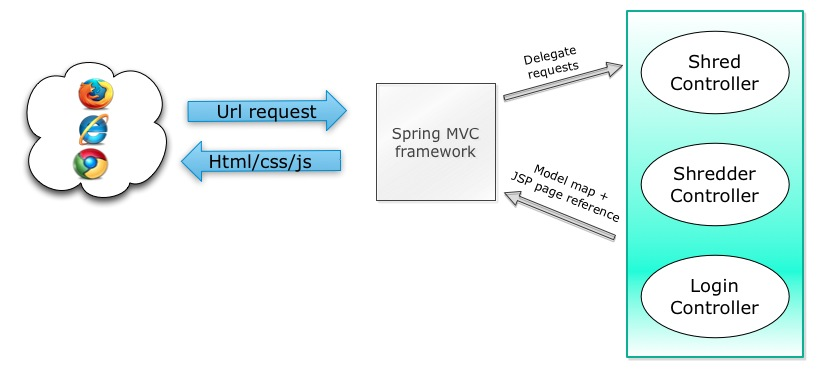
\includegraphics[scale=0.5]{images/presentationtier1.jpg}
%  \caption[sp.]
%   {The presentation tier's responsibility }
%    \label{fig:presentationtier1}
%\end{figure}
\section{The presentation layer}
The presentation layer is the first entry point in the application. Its responsibility is to handle client interactions, meaning it will handle authentication, session management, and input validation. The presentation layer is also responsible for knowing what operation to call in the domain logic layer, and it generates the views that are sent back to the client. It is built with the Model-View-Controller pattern, because this creates a nice and coherent separation of concerns. 

\subsection{Authentication}
The first entry point in a SpringMVC application is a set of interception filters. In Architecture 1.0 these filters are configured to handle authentication, access control and a bit of input validation. Users must to be authenticated in order to use any of the pages on Shredhub except the login page. Most of the authentication and access control handling is set up to be handled automatically by Spring, through the Spring security framework \cite{springsec}. Spring provides a lot of different authentication protocols, both based on standardized security protocols, and customized solutions made by third parties. For simplicity, I have chosen to use a Html form-based authentication mechanism that relies on a username, password and security-role. Other common authentication solutions used in Web apps are HTTP BASIC or HTTP Digest, or HTTP X.509 client certificate exchange. However, I find that form-based authentication fits the simple scope that has been chosen for authentication in this thesis, and it conforms to \textit{Reference-model 1.0}, because it relies on server's session handler.

The form based authentication process works by letting users enter a username and password in an HTML form on the login page. On form submit, the request is picked up by Spring's interception filters, which will look in the database for a Shredder with the given username, password. The database row for a Shredder also contains a column that represents the Shredder's user-security-role. However, for simplicity there is only one role in this app, which is the one that gives access to everything. If a row with a matching username and password is found, the framework will grant access to the user, and the user will now have access to the whole Web app. To avoid having to re-authenticate for every subsequent request, Spring will behind the scenes maintain a security-context object that is connected to the User's HttpSession. The security-context object simply indicates that the user has successfully logged in once, and is allowed to perform the given request. 
		  
\subsection{State Management}
In respect to \textit{Reference-model 1.0}, state is to be maintained on the server. 

The presentation layer is responsible for managing state associated with a User when he navigates around the app. In Architecture 1.0, this is implemented by using Spring's HttpSession object. The Spring IOC container creates one HttpSession object for every current User, which naturally is scoped at session-level. Considering that Spring offers readily available in-memory objects scoped at session-level, makes it very appropriate to use such objects as caches for data that is frequently accessed. In the Web app, I put state data either in objects that are maintained by the IOC container and scoped at session-level, or I put them directly on the HttpSession object, using a method called \textit{setAttribute(String key, Object value)}. The separation is a matter of separation of concerns; HttpSession object maintains meta data concerning the User (profile info, battle requests, battles, fanees etc), while other session-scoped objects maintains data regarding the User's page activities (e.g current shred-row, current shredder-page etc).

 Data that is used to populate views on the server has to be fetched from the database. Many of these database calls can be avoided if some of the data is stored in memory. The data could for instance be a particular set of Shreds that must be fetched especially quick in order to achieve responsive behavior, User data that is displayed often, e.g the User's name, or a list of battle requests which is meant to be visible on the top navigation-bar at all time. Shredhub needs to be very efficient and responsive, therefore solutions to avoiding repetitive and redundant database lookups has been prioritized in this architecture.The problem however, is that there is a tradeoff in how much data should be kept in memory, as maintaing too much memory might make the application slow, and in worst case lead to out of memory exceptions. Also, and this is a special case for typical Web 2.0 applications, data tend to change frequently, and users naturally want up-to-date views of the data. Hence, content regarding the Shreds and the newest Shredders on Shredhub, new fan-connections and other data that frequently changes, for simplicity shouldn't be cached. However, alternative solutions that makes it possible to cache such data is to some extend possible, for example by implementing push-based public-subscribe service that signals the cache to update whenever an update is made. Or alternatively a pull based solution where some service frequently pulls the database for new updates. A very simple proposal for such a solution is given later in this section.

Given below I have addressed two different collections of data objects that are frequently accessed in the application, together with an indication of how frequent the object changes, how often it is accessed, and the decision of wether they are cached in the User's session or not:
	
	\begin {enumerate}
	\item{} Data that is fetched in each Http request:
	
	\begin{tabularx}{\linewidth}{ | X  |l | l | l |}
	    \hline
	    \textbf{Data object} & \textbf{Changes}  & \textbf{Displayed} & \textbf{Cached in session}\\ \hline
	    The User's username &  Never & Always & Yes\\ \hline
	    The User's fanees & Moderate & Always & Yes\\ \hline
	    List of battle-requests for the User & Moderate & Always & Yes \\ \hline
	    The User's unique ID & Never & Always & Yes \\ \hline
	    \end{tabularx}
	
	\item{} Data that is accessed  frequently
	
	  \begin{center}
	\begin{tabularx}{\linewidth}{ | X  |l | l | l |}
	    \hline
	    \textbf{Data object} & \textbf{Changes} & \textbf{Displayed} & \textbf{Cached in session} \\ \hline
	    User's profile details, like address, guitars, age, email, birthdate, etc & Seldom & Moderate & Yes \\ \hline
	    The User's current battles & Moderate & Often & Yes \\ \hline
	    
	    The rows of Shreds that are displayed in the shred-pool & Often & Often & Partly \\ \hline
	    
	     Page navigation data, e.g page numbers and Shred-row numbers & Moderate & Often & Yes\\ \hline
	    The shred-news list & Often & Often & No\\ \hline

    	    Shred, Battle or Shredder the User just looked at & Moderate & Often & No\\ \hline
	   \end{tabularx}
	\end{center}
	
	\end{enumerate}	
	
In general, data objects that are frequently accessed and that is special to the User, should, and is being cached in the session. 

\paragraph{Table 1}:
 The reason I store everything in this table is because this data is accessed very frequently, it only addresses the User, and it doesn't change often. All of these objects are fetched when the User logs in, and for simplicity, I never pull the database for updates concerning this data. Hence, for instance if the User gets a new battle request during the session, it won't be visible until the next time he logs in. This is simply because I didn't have time to implement a pull/push based service, and I consider this behavior good enough for this thesis. 
 
\paragraph{Table 2}:
In the second table I have chosen to store the User's profile details, the User's current battles, and navigation data. The latter is just a set of small integer numbers that controls for example the page number for the list of Shredders the User is currently at, or which row number in a particular Shred-row on the shred-pool is the User currently at. This could also be stored in the Urls, however I chose to keep the Url's clean of state information, and instead maintain this state info on the server, as the Url option to a higher extend addresses \textit{reference-model 2.0}. The data objects mentioned here do not change very often, and are most likely small in size. These are also fetched when the User logs in, and aren't updated, unless update is made by the User himself. This could be for instance if the User updates his profile details, adds a new fanee or starts a new battle. In this case I eagerly write to the database, and at the same time update the cache.


The set of Shreds that are displayed in the shred-pool are only partly cached: the shred-pool is made up of multiple rows of Shreds. Each row consists of 3-5 Shreds, depending on which Shred-row it is, and the User can click a next button change the particular row to a new set of Shreds. Now, for each row, the server fetches a set of 20 Shreds from the database, and maintains these in a session-cache (or buffer). Whenever the User clicks on the ``next'' button in a row, the server checks the cache for that row to see if the next row of Shreds lies within the buffer. If they do, the row is moved one row-size, and this new row of Shreds are displayed. If not, the server fetches another 20 Shreds from the database and displays the first row from the new buffer. By using this buffer of Shreds for each row, the server avoids many calls to the server, which is very important in order to get quick and responsive behavior when the User clicks the next button. The buffer could also be bigger, but then again there is a tradeoff in how big the cache can be without influencing performance. 

The last two rows in table 2 concerns data that changes often and should always be up-to-date. In this case it is not worthwhile caching anything, considering the data must always be fetched eagerly from the database in order to be sure to have up-to-date data. The last row concern objects that could actually be saved in the cache, considering there is a chance the User might want to look at them again shortly, and in cases where the data is not likely to have been update yet. However, again, for simplicity I have chosen not to cache. 

\subsubsection{A Simple Cache Proposal}
As caching is very important for maintaining good performance , a simple caching solution for Shreds and other data that frequently changes is given in the following outline:
\textit{The caching scenario works by having a Java container object scoped at session-level, that maintains a HashMap of cached objects. The objects are be referenced by their database ID, so that whenever a request comes in for either a Shred, Battle or a Shredder object, the client of the cache container checks if the object with the Id is there. If so, it is returned, if not, the object is fetched from the database, put in the HashMap and returned to the requestor. To maintain updated values, there could be a background process that is triggered every time the cache is checked. For every object in the HashMap, the background process checks the database for the object with the given Id, and compares the value of the time-of-last-update field. If the object in the database has a newer time value, the database object is swapped with the outdated object in the cache. Spring provides many different implementations of an interface called TaskExecutor, which is able to perform background jobs both asynchronously and in concurrent fashions. An alternative to fire of the background job every time the cache is accessed is to use a Scheduled job that executes the background process every n seconds. } 

This cache could be used both for a User's session, such that data that concerns the user himself (for example the set of Shred, or Shredder recommendations that are displayed in the shred-pool ), or it could be maintained as a general cache for every user. This would maintain data that is frequently accessed by everyone, for example the list of the top rated Shreds that is displayed in the login page and in the shred-pool. Unfortunately I have not had the time to implement such a solution. 

It is worth mentioning that there are many alternatives for how data can be cached in memory in order to avoid consulting the database. Another approach I could have taken is to use a third party service like Memcached,\cite{memcached} which is a highly efficient in-memory storage of data that can be placed on the same machine as the application server, or (as recommended) distributed to multiple machines. This would extend the caching capability of Shredhub. Unfortunately, I did not have the time to integrate such a service for this thesis. 

\subsection{Input Validation}
Input validation is both part of the presentation layer, which addresses form-input rules, and the domain logic layer, which enforces business rules of the input data. In the presentation layer, validation is usually the first thing that happens once a Url request enters the server. Validation is always performed by applying positive filtering, meaning I specify what's allowed, and forbid everything else. Another approach is to do negative filtering where the input scanned for illegal patterns. However the latter approach is not as secure because it is hard to imagine all possible attack-forms.\cite{sqlinjection} Also, new forms of attacks might be invented in the future. However, positive filtering has the downside that it might be to restrictive.

Mainly I have two ways of verifying user input in the application. One of them is to enforce validation rules directly onto the variable in the domain object classes, I.e the Shredder class will contain validation rules concerning its data variables, the Shred class contains validation rules concerning its variables etc. This feature is something that's provided by Spring, using keywords in the domain classes that are automatically picked up by Spring. This validation is performed whenever the User creates a new domain object, such that the validation is executed before control is handed to a controller. The other way validation is done is by manually checking the Html form-input illegal input, or access rules. For example the controller often checks that the User stored in the session is allowed to perform a given business operation, or that a video file is sent when the User wants to add a new Shred. 

An example of validation rules applied to a domain object is displayed in the code below. This shows the use of regular expressions and other rules to define the format of the data that is allowed for a Shredder. The annotations (referenced by the ``@'' character) are picked up by SpringMVC whenever a new Shredder object is created. Spring will then check that the data entered matches the rules, if not, an error is generated. Hence positive filtering.
	
\begin{lstlisting}
	public class Shredder implements Serializable{
		
	        @Size(min=3, max=20, message=
	    		    "Username must be between 3 and 20 characters long.")
	     @Pattern(regexp="^[a-zA-Z0-9\\s]+$",
	     	message="Username must be alphanumeric")
	     private String username;
	     
	     @Pattern(regexp="[A-Za-z0-9._%+-]+@[A-Za-z0-9.-]+\\.[A-Za-z]{2,4}",
	    	        message="Invalid email address.")
	     private String email;
	     
	     @Size(min=6, max=20, message="Passwords must be between 6 and 20 characters long.")
	     @Pattern(regexp="^[a-zA-Z0-9\\s]+$",
	 	        message="Passwords must be alphanumeric")
	     private String password;     
	    
	     .... // other fields
	     
	     }
\end{lstlisting}
Before I went with this approach, I tried to implement negative filtering. Here, I created a custom validator class that would perform negative filtering on the user data. The validator's validation function is executed before the appropriate controller handler is called. The validator function would inspect the input to find potential illegal data. If any potential violation characters or patterns were found (for instance the sequence " ' OR 1=1; SELECT ...; -- ", which is a typical SQL-injection attack) I created an error message that is delivered to the controller function that is to execute next. This approach was very cumbersome, because it had to test for many different text patterns, and also, it is hard to know every possible set of illegal inputs.


\subsection{Controllers}
Controllers are first-class citizens in the presentation layer, who's responsible for processing URL requests. These components represents the Controller part of MVC. Controllers are Java classes that are mapped to specific a specific Url pattern. A simple approach is to have one controller class that is used for every Url supported by the Web app. However, this is not very maintainable, as the class would  grow exceptionally large, and have many responsibilities. Other solutions are for instance to have one controller class for every View, or one for every domain object. I have chosen to implement something in between. I chose to implement one controller class for each main resource/domain in the application, in addition to one controller for the login, and shredpool view (simply called the login controller). In the table below we can see all the controllers in Architecture 1.0, together with some example controller handlers and their respective responsibilities. Although not displayed in the table, note that each controller handler is mapped to a unique Url.

\begin{center}
    \begin{tabular}{ |  l  | p{6cm} |  l  |}
    \hline
	\textbf{Controller handler} & \textbf{Responsibility} & \textbf{View returned} \\ \hline    
    \multicolumn{3}{|c|}{HomeController} \\ \hline
    loginPage() & Handles requests for the login page. Fetches the top-rated Shreds from the database and renders the login page & The login view \\ \hline    
    
    loginSuccess() & Called when authenticating the User succeeds. Populates the session cache with data fetched from the database & None: redirects to www.shredhub.com/theshredpool \\ \hline
    
    theShredPool() & Fetches from the database the set of Shreds and all the shred-news that are to be displayed in the shred-pool. & The shred-pool view \\ \hline
    
      showShredInShredPool() & Given a Shred id, the Shred is fetched from the database and renders the shred-pool view so that it displays the Shred as a pop-up window on top of it & The shred-pool view \\ \hline
    
    \multicolumn{3}{|c|}{ShredController} \\  \hline
   
     createShred() & Creates a new Shred, saves to the database & The shred-pool \\ \hline

     postComment() & Ajax supported function that given a shredId and comment-text, adds a new comment to a Shred where the comment-owner is set to the id of the User (stored in session) & None \\ \hline
     
    \multicolumn{3}{|c|}{ShredderController} \\      \hline
getShredders() & Fetches the next page of 20 Shredders that are to be displayed in the list of Shredders view. The page number is maintained in the session object & The shredders view\\ \hline
followShredder() & Adds a new fanee to the User's list of fanees. Updates the session-cached list of fanees for the user  & The shredders view \\ \hline

newShredder() & Creates a new Shredder. Stores it in the database & The login view \\  \hline

 \multicolumn{3}{|c|}{BattleController} \\ \hline
 getBattle() & Fetches a battle object given a Battle Id & The battle view \\ \hline

newBattle() & Called when a Shredder accepts a Battle request that is being kept on the session object. Creates a new Battle object. Stores it in the database & The shred-pool view \\ \hline

getBattles() & Called when a Shredder accepts a Battle request that is being kept on the session object. Creates a new Battle object. Stores it in the database & The shred-pool view \\ \hline


    \end{tabular}
\end{center}

This controller granularity is very intuitive and coherent, and it makes it easy to extend the application with more actions. For example if I was to implement a new function for the application, say, the use case: ``remove a fanee-connection'', this would naturally be implemented as a new controller handler function inside the ShredderController class. I could however, have created even more fine-grained controllers, say a ShredPoolController, a FanController, or even a BattleRequestController, but I feel the amount of controllers fits the application quite well. 

\subsubsection{Control Flow}
In this section I will describe what happens in the controller when a Url request comes in. An example controller, and a controller handler is given in the code below. Extra comments are added to explain important things.
		
\begin{lstlisting}

// Handles all Url requests for www.shredhub.com/shredder*
@RequestMapping("/shredder")
@Controller
public class ShredderController {
		
	// Entrance to the domain logic layer
	@Autowired
	private ShredderService shredderService;
			
	// Handles a url requests for www.shredhub.com/shredder/<someFaneeId>/?action=follow
	@RequestMapping(value = "/{faneeId}", method = RequestMethod.POST, params = "action=follow")
	public String followShredder(@PathVariable int faneeId, Model model, HttpSession session) {
		Shredder user = (Shredder) session.getAttribute("user");
		List <Shredder> shreddersFanees = (List <Shredder>) session.getAttribute("fanees");
		try {
			
			// Delegate to the business operation
			List <Shredder> updatedFaneesList = shredderService.createFaneeRelation(user(), faneeId, shreddersFanees);
			
			// Update the session 
			session.setAttribute("fanees",updatedFaneesList);
			
			// Return the view that displays a list of 20 Shredders
			return this.getShreddersAndReturnShreddersView(model, session);
			
		} catch (IllegalShredderArgumentException e) {
			// Something wrong happened in the business operation. Return the error-page view
			model.addAttribute("errorMsg", e.getMessage());
			return "errorPage";
		}
	}}	  
\end{lstlisting}
This particular controller handler is triggered when the User clicks an anchor tag with the link given in the comment above. The shredderService reference is the gateway to the domain logic layer. SpringMVC's IOC container will inject a concrete implementation of ShredServices, because the pointer is annotated with an @Autowired field, which is picked up by Spring when the application is started. When the request comes in, the controller handler fetches the user from the session, because the business operation needs the User's Id and his corresponding list of fanees to check if the User is already a fan of the Shredder with id=<faneeid>. Note that if this Url request would be a form submit that contains user generated input data, the controller would first check the result of the input-validation process done by the interception-filters. If the validation process found en error, the controller handler return an error page immediately, instead of calling the logic layer. Anyhow, if a business operation is called, the controller would upon return catch any exception that might have occurred somewhere down the line. For example if the User is already a fan of the other Shredder. Note that I could have chosen to run this check inside the controller handler before I call the business operation, but this is strictly speaking a business rule that belongs in the business logic layer. If an error is found, the a Model object is populated with the data that is to be rendered together with the error view. The Model object represents the Model in MVC. This object will be used to contain the data that is injected into the views that are sent back to the user. Going further, if the business operation that was called succeeded, the controller calls a function that does the following:
\begin{enumerate}
\item{} Set p = the current page number stored in the HttpSession object
\item{} Ask the logic layer to fetch a list of 20 Shredders, starting from page num = p
\item{} Put the result list on the Model : model.addAttribute(``shreds'', resultList)
\item{} return the String ``shredders''
\end{enumerate}
The returning String is picked up by SpringMVC's View Resolver which I have configured to map my Java Strings to names of Jsp files. Hence the View Resolver will look for a view names ``shredders.jsp'', or ``errorPage.jsp'' in case the error view is returned from the handler. How the views are generated is explained in the next section. The reason I do this last part in a separate function is because it is called by other controller handlers as well. Also, the reason I chose to return the shredders page, is because it is from this page the User initially clicked the follow link, and therefore the controller just returns the same page as the user was in.
 
\subsection{Views}
Views represent the V of MVC. In Architecture 1.0, Views are implemented with the Java Server Pages (JSP) technology. JSP is fully supported by SpringMVC's template engine, and is a popular choice for dynamic view generation. The reason I chose JSP is because it has good support for many tag libraries, which extends the language features that can be used in the Views, and it makes it easy to integrate  the domain objects' data fields into the view. Also, it has a nice and intuitive syntax, that is more Java-like then other template technologies (for instance Velocity or Freemarker). However, one could argue that choosing Velocity or Freemarker is a better approach because its syntax is more appealing to non-Java developers. 

It is considered best practice to avoid implementing business logic in the views. \vref{Johnson04} View logic, on the other hand (code that generates the user interface), should only be done in the presentation layer, because it has got nothing to do with either the domain logic layer, or the datasource layer in terms of code-responsibility. To blend these responsibilities together would result in tight couplings between how the page looks like, and the data it operates on. This is one of the reasons I chose to implement the MVC pattern, because it nicely separates these concerns, making it easy to change the view without harming the business logic, and likewise to let the models be unaware of its presentation, so the presentation and models can change independently. Note that the models are implemented in the domain logic layer, but are used by controllers and views in the presentation layer.

\subsubsection{Main Components}
There is one View for each page in Shredhub. These are:
\begin{enumerate}
\item{} The login view
\item{} The shred-pool view
\item{} The shredders view
\item{} The shredder view
\item{} The Battle view
\end{enumerate}

Also, there are some views that are re-used in the above views:
\begin{enumerate}
\item{} the header view
\item{} the footer view
\item{} show shred view
\end{enumerate}

Each of these views are implemented as a jsp file, e.g login.jsp. The last three views in the list are injected into the other views using special JSP syntax, in order to avoid view duplication. The views contain static HTML tags that never changes, some Ajax functions written in JavaScript, and external links to CSS files and JavaScript libraries. JSP tags are used to inject the domain objects into the View by referencing to the Model object that is populated with data in the controllers. A simple example of the shredders view is displayed below:

\begin{lstlisting}[language=html]
<html>
<body>
	<jsp:include page="header.jsp" />	
	<h1>Shredders</h1>		
	<form action=``searchForShredder''>
		<p>Search for a Shredder </p>
		<input type="text"/>
	</form>
		
	<c:forEach items="${shredders}" var="shredder" varStatus="i">
		<div class="shredderInList">
			<img src="<c:url value="/resources/images/profiles/"/>$								{shredder.profileImagePath}"	alt="Profile img">

			<a href="<c:url value='/shredder/'/>${shredder.id}">${shredder.username}</a>
			<p>${shredder.description}</p>
			<p>Level: ${shredder.level}</p>
		</div>
	</c:forEach>
	<a href="<c:url value='/shredder/'/>nextPage">Next</a>
	<jsp:include page="footer.jsp" />
</body>
</html>
\end{lstlisting}
As we can see, the special template syntax is indicated with the ``<c:'' and ``$''. The c tags represents things like loops and conditionals, while the $ tag directly refers to objects that the controller handler has put on the Model object (as we saw previously). Here, we use a c:forEach to loop through a list of shredders that were given to us in the controller that returned this particular view. After a controller handler finishes, and the View Rendered gets this view together with a Model object, it compiles the view by executing the special JSP syntax, and outputs a fresh HTML page. SpringMVC sends the Html page back to the client. 
 
The next example shows the one and only place in the app where Ajax is used to implement dynamic in order to avoid fetching a complete view from the server. The example shows the a simplified version of how a Shred is displayed. Now, if the User rates or comments the Shred, the new result (I.e updated rating value or the new comment) has to be displayed very quickly in order to achieve proper responsive behavior. This could be solved the usual way by using form-submits, but in this case, this is not good enough, because it results in a complete page refresh in the browser. Everywhere else in the app however, regular form submits are ok.

\begin{lstlisting}[language=html]
	<srcipt type=``text/javascript''>
		function commentShred(shredId, commentText) {
			// Create the url that calls the controller handler on the server
			var baseUrl = "<c:url value='/shred/'/>" + shredId;
			var url = baseUrl + "/comment/?text=" + commentText;
	
			// Send the Ajax request to the server as a Http post request.
			// The result from the server is the Shred with the list of comments 
			// updated with the new comment 
			$.post(url,
			
			// This function is called when the server's response gets back
			function(shred) {				
				// get the last comment from the shred, I.e the one the User just created
				var lastComment = _.last(shred.shredComments); 
				
				// Create a comment as an html string,
				// that is to be injected into the DOM tree
				var htmlString = '<tr><td>' + lastComment.text + 
       			        '</td><td>' + lastComment.commenter.username + 
				'</td><td>' + new Date(lastComment.timeCreated).toUTCString() + '</td>'+
				'<td><button type="button" class="close"
				 onClick="deleteComment(' + last.id + ', ' + data.id + ');" >x</button></td></tr>'
				 
				 // Append the Html to the table of comments
				$('#commentTable tbody').append(htmlString);
			});
	}
	
	function rateShred(shredId, commentText) {
		// I have omitted the source code for this example,
		// But it's very similar to the function above
	}
</script>

	<div class="videoView">
		<video id="videoInModal" src=``<c:url value="/resources/videos/"/>''$										{shred.videoPath''</video>
			<p> Created at: ${shred.timeCreated} </p>
			<p">Number of raters:${shred.rating.numberOfRaters}</p>
			<p>Rating:${shred.rating.rating}</p>
			
			<p>Rate it:
			 <input type="range" id="rateValue" min="0" max="10" name="rating" value="5">
			<button id="rateButton"
				onclick="rateShred($('#rateValue').val()); return false;">
			Rate</button>
			
			<p>Write a comment</p>
			<input type="text">
			<button id="commentButton"
			onclick="commentShred($('#shredCommentText').val());
			 return false;">
			 Comment</button>
			
			<h3>Comments</h3>
			<table id="commentTable">
			<thead>
				<tr>
					<th>Text</th>
					<th>By</th>
					<th>At</th>
				</tr>
			</thead>
			<tbody>
				<c:forEach items="${currShred.shredComments}" var="c">
					<tr>
					<td> ${c.text} </td>
					<td> ${c.commenter.username} </td>
					<td> ${c.timeCreated} </td>
					</tr>
				</c:forEach>
			</tbody>
			</table>
	</div>
\end{lstlisting}

In order to display the video, I have chosen to use the HTML5 tag <video>. This tag makes the browser fetch the video from the Url defined in the ``src'' attribute of the video tag, display a video frame, and provide a play button that the User uses to start the video. Another alternative to show videos is by using streaming technology, where raw bytes are transferred in real time while the user watches the Shred. This way the whole video doesn't have to be fetched before it can start to play. However, the performance benefits with choosing either of these approaches is out of scope for this project, so I won't dig into it. 

Its worth noticing the \textit{onclick} attribute on the rate- and comment buttons. These are JavaScript handlers that are triggered when the user clicks either of the buttons. When the onClick events are fired, the browser will call a JavaScript function (one of the two we see in the code example) that uses Ajax to submit the request to the server. The result from the server is the updated Shred object which is used to populate manipulate the DOM tree to display the updated value. As stated in previous chapters, the JavaScript functions are independent, and self contained. An unfortunate property here is that the JSP view now contains Html, JSP tags and JavaScript. Three languages in the same file, which makes the code somewhat messy. I could put the JavaScript files in a separate source file, but the JavaScript would still have to use both Html and Jsp tags. 

\subsection{Summary of The Presentation Layer}
The presentation layer is built with MVC. Form submits and link actions are picked up by a specific controller handler on the server. The handler performs validation, state management, and delegates to a business function in the domain logic layer.

Models are implemented in a lower layer, but are heavily used by the presentation layer. After a business operation is performed, the Controllers are responsible for choosing which Model objects to send to a View, and the Views can access the data in the Model through special JSP syntax.

The presentation layer depends heavily on state implemented as session-scoped objects, but due to the nature of Web 2.0 applications, which requires data to have up-to-date values at all time, there isn't very much data to cache. Also, I acknowledged that there should have been a dedicated caching system in this architecture, but this was out of project scope to implement.
			
\section{The Domain Logic Layer}
The domain logic layer is the part of the application that receives a specific action from the controller, and performs the necessary business logic needed to complete the action. Now, since the responsibility of the logic layer is to implement the business logic in the application, it is important that this software layer is flexible. Flexibility, means that it can be relatively easy to add new features without harming anything else in the source code, and it should be easy to modify the already existing code. To achieve this, I needed a coherent design, preferably built with design patterns that gives a proper structure to the software architecture. To organize the layer, I have chosen to use the service layer design pattern \cite{poea}. This pattern creates a boundary into all of the application's business logic operations, by dividing the application into logical abstractions. Each abstraction represents the business operations that operates on a particular resource, or domain in Shredhub (e.g a Battle, a Shredder, or a Shred). However, this is not to be associated with the application's domain objects which concerns the domain resources' data, not functions. Instead, the service abstractions wraps the set of operations that are supported for each resource. Hence, each service class has a set of service functions. The list of service classes with some essential service functions are given below:
		\begin{enumerate}
			\item{} BattleService 
				\begin{itemize}
					\item{} getBattleWithId
					\item{} getOngoingBattlesForShredderWithId
					\item{} acceptBattleWithId
				\end{itemize}
			\item{} ShredderService
				\begin{itemize}
					\item{} addShredder
					\item{} getShredderWithId
				\end{itemize}	
			\item{} ShredNewsService
				\begin{itemize}
					\item{}getLatestShredNewsItems
				\end{itemize}
			\item{} ShredService
				\begin{itemize}
					\item{} getFanShreds
					\item{} getAllTags
					\item{} getShredsForShredderWithId
				\end{itemize}
		\end{enumerate}

\begin{figure}
		  \begin{center}
		\fbox{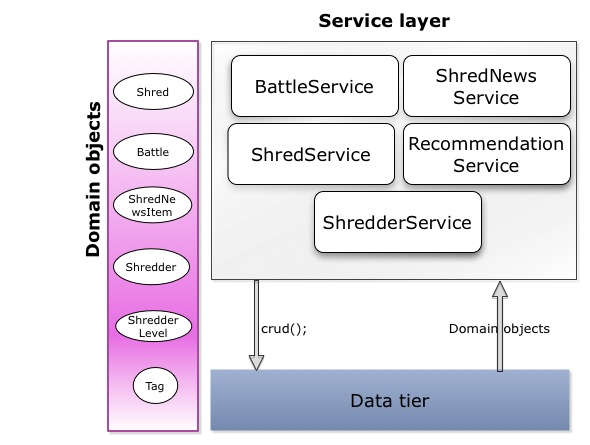
\includegraphics[width=14cm] {images/middletier.jpg}}
		% Kommandoen \fbox tegner en ramme.
		\end{center}
		\caption{The domain logic layer and its connection to the datasource layer}\label{fig:middletier}
\end{figure}

\subsection{Service Functions and Domain Objects} 
The service functions are called by the controllers in the presentation layer. An overview of the domain logic layer and its responsibility relative to the data source layer is given in figure \vref{fig:middletier}. The figure shows all the service abstractions, and the set of domain objects in Architecture 1.0. The domain objects represents the application's core resources, implemented as simple Java classes with no logical functionality, just attributes with accessor methods. The domain objects I have chosen to implement are Shred, Shredder, Battle and BattleShred. These objects have references to each other, and are used across all three layers in the application, making them the one means for communicating the domain in the application. The logic layer sends domain objects to the datasource layer in order to persist them. When the logic layer needs data from the datasource layer (e.g the database), the datasource layer will respond with domain objects.

An alternative architecture I could have chosen instead of the service layer pattern, is the table module pattern \cite{poea}. In the table module pattern,  all the SQL rows in the database gets a separate class that is responsible for performing the operations that are made on each row. However, this approach is very tight coupled to the database. Another alternative is to use the domain model pattern, which is often implemented in Ruby on Rails apps. Here, the domain objects would be responsible for performing business logic on themselves, and manipulate the database. This is a good approach, but the domain objects might end up being very big, with lots of responsibility. I prefer the solution of having a separate service class for each logical application abstraction, where the service functions performs all the necessary business logic for a given action, and the domain objects are plain data holders. However, a hybrid is also possible, where the domain objects implement parts of their logical behavior. However, I prefer to separate these concerns.
	
	
A final thing to point out is that because some service operations perform multiple  subsequent database transactions, each such service operation must be atomic. Spring achieves this behavior very elegantly by letting classes be declared as transactional, meaning every service operation in that class will be transactional (i.e have atomic behavior). In effect, if a database operation fails during a set of multiple database operations, the whole transaction is rolled back to the initial state. Hence atomicity (the A in ACID) is provided.  
	
\subsection{Data Flow}
Most operations in the domain layer follows the same structure; some data is fetched from the datasource layer, this data is manipulated together with the data it got from the calling controller handler, and the result is written back to the database. Also, sometimes the newly updated data is returned back to the controller, so that this can be rendered in a new view. If an error occurred along the way (for instance if illegal data was sent from the controller), an exception is thrown and picked up by the controller so it can return an error view. An example of a typical business operation is given in the code below:
	
	\begin{lstlisting}
	@Service
	@Transactional( readOnly=true )
	public class ShredServiceImpl implements ShredService {
	
		// Data source reference
		@Autowired
		private ShredDAO shredDAO;	
		
		/**
		* This adds a new rating to a Shred. 
		* When a shred is rated, the shred will gain a higher total rating, and
		* the shredder who made the shred also achieves
		* more experience points. Note that I don't check if the one who rates the 
		* Shred is the one who created it. This is a business rule that should be implemented
		* here, inside the business operation. However, for simplicity I have avoided it.
		*/
		@Transactional ( readOnly = false )
		public void rateShred(int shredId, int newRate) throws IllegalShredArgumentException {
			Shred shred = shredDAO.getShredById(shredId);
			if ( shred == null ) {
				throw new IllegalShredArgumentException("Shred with id: " + shredId + " does not exist");
			}
			if ( newRate < 0 || newRate > 10 ) {
				throw new IllegalShredArgumentException("Illegal rate value!");
			}
	
			// Here I could use the domain model pattern so that the
			// shred object itself knows how to set its own rating.
			// But I choose to follow the service layer pattern, where all the logic
			// is implemented in this service operation
			ShredRating currentRating = shred.getRating();
			currentRating.setNumberOfRaters(currentRating.getNumberOfRaters() + 1);
			currentRating.setCurrentRating(currentRating.getCurrentRating()+newRate);
			
			// store the result in the database
			shredDAO.persistRate(shredId, currentRating);		
			
			// Fetch the complete owner (Shredder) object from the database
			Shredder shredder = shredderDAO.getShredderById(shred.getOwner().getId());
			
			// Uses a utility class that is shared by all the service classes
			// in order to update the shredder level
			UpdateShredderLevel usl = new UpdateShredderLevel(shredder, newRate);
			usl.advanceXp();
			
			shredderDAO.persistShredder( shredder);
		}
	}
	\end{lstlisting}
This function is called by the controller handler that receives requests for adding a new shred rating. At first, it tries to fetch the Shred from the database, before it performs some input validation on the data it received. If all went well, the service function will set the new rating and persist the result back to the database. Then it will fetch the Shredder who initially created the Shred in order to increase the Shredder's experience points. Finally it will persist the Shredder back to the database. Note that just like the presentation layer did with the domain layer, the domain layer  delegates every persistency operation to the data source layer. The data source layer is reached through special references called DAOs. This is a nice separation of concerns, because the service functions only have to worry about the business rules, not how the data is persisted. Also, note that the operation in this example has to be atomic, because the function has multiple subsequent calls to the database. For example, if an error is made during the call to \textit{shredderDAO.persistShredder(shredder)}, the whole transaction will be rolled back to the state that was before \textit{rateShred} was called.

\subsection{Summary of The Domain Logic Layer}
The domain logic layer implements the domain of the application. The layer is divided into two; a service layer that implement business logic operations, and the domain objects which wraps the domain into self-contained data holders. The domain is divided into three abstractions; a Shred, Shredder, and a Battle class. The services are separated into a ShredService, ShredderService and BattleService class. The services forms a facade that is used by the controllers in the presentation layer. The services delegates to the data source layer for persistence.

	
\section{The Data Source Layer}
The datasource layer is the part of the application that receives a particular CRUD command from the domain logic layer, executes a SQL operation on the database, maps the result to a domain object and returns the result back to the business logic layer. I have chosen to use a PostgreSQL database, because it is open source, highly efficient, popular in the web industry, well documented, and most importantly, I know the database quite well. Also, I have chosen not to use an ORM mapping tool, but rather build Java functions that talks directly to the database using Strings as queries, and mapping query results manually to Java objects. There are many good ORM technologies I could have chosen to use, for example Hibernate, and JPA, which would hide the complexity of serializing Java objects to SQL, and the opposite, and not having to deal with SQL. However, these technologies does not give me the control I need to fine-tune, debug and create flexible and complex queries. A tradeoff though, is that writing SQL with java statements tend to get messy, especially when the queries gets many and complicated. I do however value the control one gets by explicitly writing every query with SQL. Obviously performance is important in this project, which makes it a big benefit to be able to take advantage of PostgreSQL's proprietary features.
		
\subsection{SQL Implementation}
The Java driver that connects to, and sends queries to the database is called JDBC. Spring provides a nice wrapper around the JDBC framework through a class named JDBCTemplate. This class takes care of all the boilerplate code like resource management and exception handling that is required when operating with JDBC. The SQL tables that represents the three central domain objects in the application is showed in the example below: 
		
\begin{lstlisting}[language=SQL]
	CREATE TABLE Shredder (
		Id				serial PRIMARY KEY, 
		Username		varchar(40) NOT NULL UNIQUE,
		BirthDate			date NOT NULL CHECK (BirthDate > '1900-01-01'),
		Email			varchar(50) NOT NULL UNIQUE,
		Password			varchar(10) NOT NULL
		Description		text,
		Address			text,
		TimeCreated		timestamp DEFAULT CURRENT_TIMESTAMP,
		ProfileImage		text,
		ExperiencePoints	int	DEFAULT (0),
		ShredderLevel		int DEFAULT (1),
		Guitars			text[],
		Equiptment		text[]
		
	);
	CREATE TABLE Shred (
		Id				serial PRIMARY KEY,
		Description		text,
		Owner			serial REFERENCES Shredder(Id),
		TimeCreated		timestamp DEFAULT CURRENT_TIMESTAMP,
		VideoPath		varchar(100) NOT NULL,
		ShredType		varchar(30) DEFAULT 'normal' CHECK (ShredType ='normal' or ShredType = 'battle')
	);	
	CREATE TABLE Battle (
		Id				serial PRIMARY KEY,
		Shredder1		serial REFERENCES Shredder(Id),
		Shredder2		serial REFERENCES Shredder(Id),
		TimeCreated		timestamp DEFAULT CURRENT_TIMESTAMP,
		BattleCategory		serial REFERENCES BattleCategory,
		Round			int DEFAULT 1,
		Status			varchar(30) DEFAULT 'awaiting' CHECK (Status ='accepted' or Status ='declined' or Status='awaiting');
	);	
\end{lstlisting}

In addition there are many-to-many relations between Shredders and Shreds, Shredders and Battles, and Battles and Shreds (actually BattleShreds, but they almost identical). Its important to mention them, because it requires the data source layer to perform complex join operations when fetching data from the database.

Now, there are lots of other smaller tables in addition to these, but these are the most essential. To perform the CRUD operations, I have chosen to structure my data tier around the Data Access Object (DAO) pattern. In this pattern, separate DAO objects are responsible for performing the relational data mapping on behalf of a particular domain object. This way the domain objects has no clue on how to persist themselves. An alternative to this is to use the Active record design pattern, where each domain object contains persistence code. However I prefer to keep this behavior separated from the domain objects as they would grow quite large and complex if they where to contain all the necessary object relational mapping code. Figure \vref{fig:datatier}
	\begin{figure}
	  \begin{center}
	    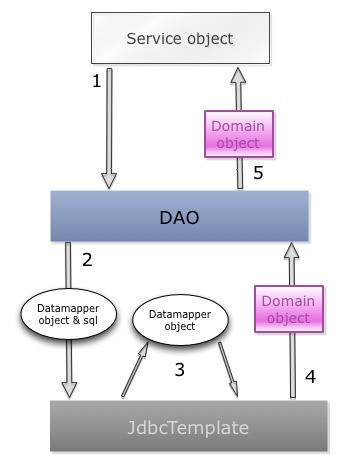
\includegraphics[width=0.5\textwidth]{images/datatier.jpg}
	  \end{center}
	  \caption{Data access pattern in the data tier}  \label{fig:datatier}
	\end{figure} 
	shows how object relational mapping is done in the data tier. Here's what happens when the domain logic layer asks the datasource layer to perform a CRUD operation (e.g a Read operation).
		
\begin{enumerate}
\item{} The logic layer calls a persistence function on a particular DAO object, for instance \textit{shredDAO.getShredById(int shredId); }
\item{} The DAO class uses a JDBCTemplate instance (injected by the Spring IOC container) to delegate the boilerplate behavior, for example getting a database connection. The JDBCTemplate is also responsible for executing the database query itself, provided that it gets a SQL statement from its caller. For instance: 
	\begin{lstlisting}
	@Service
	public class ShredDAOImpl implements ShredDAO {
	
		@Autowired
		private JdbcTemplate jdbcTemplate;
		
		public Shred getShredById(int shredId) {
			String sql =  "SELECT * FROM Shred s,Shredder sr WHERE s.Owner = sr.Id AND s.Id = ?";
			return jdbcTemplate.queryForObject(sql, new Object[]{shredId}, new ShredMapper());
		}
	}
	
	\end{lstlisting}
\item{} The JDBCTemplate is built with the template method design pattern, meaning it does callbacks to a mapper object provided by the caller. In the above code, the callback calls a function in the ShredMapper class. This class knows how to build a Shred object given the result from a database query that the JDBCTemplate executes. An example of how a ShredMapper class might look like is given below:
Example:
\begin{lstlisting}
public class ShredMapper implements RowMapper <Shred>{
	
	public Shred mapRow(ResultSet rs, int rowNum) throws SQLException {
		Shred shred = this.setConcreteShredder();
		shred.setId(rs.getInt("id"));
		shred.setDescription(rs.getString("Description"));
		shred.setOwner( new ShredderMapper().mapRow(rs, rowNum) );
		// Another template method!
		this.addConcreteBehavior(rs, shred, rowNum);
		return shred;
	}
}

\end{lstlisting}
Notice that I also use the template method pattern to enable customized mapper functionality that can be overridden by subclasses of the ShredMapper class. This is done with the BattleShredMapper, which extends the ShredMapper class, and hence overrides setConcreteShredder() and addConcreteBehavior(). 
	
\item{} The domain object created by the mapper is returned from the JDBCTempate back to the DAO object, which depending on the type of query might catch an exception to provide nice feedback to the service function. An example might be thrown by the DAO if a Shred with the given Id does not exist.
\item{} Finally the DAO function returns the domain object back to the middle tier. 
\end{enumerate}	
	
\subsection{Storing Video Files}
Media content is a central part of the application, since the primary purpose in the application is to share videos of people playing guitar. The videos have a maximum size of (x) bytes, because Shreds are supposed to be short (less then one minute). If a user tries to upload a file that is bigger then this, then an error message is given to the user. 
	As mentioned in the presentation layer section, the whole video is downloaded to the clients web browser before it can be played. It is therefore important to offer efficient uploading speed from the application's backend. As for now, I store the videos locally on the machine that is hosting the application, inside a folder that is publicly available for the users. This has some unfortunate drawbacks. One is that the users can directly access which ever files they want on the server, if they know the url for the video. The path to where the video's are stored can be seen if one inspects the HTML source code that is sent to the client's browser. The user could simply guess the name for a movie, and try to fetch it from the server. A second problem by having no protection of the videos is that it would be easy to do overflow attacks, where an attacker simply asks for a whole lot of videos until the server breaks down. A third problem is that storing the files on the machine that hosts the server requires a lot of storage space on that particular deployment server. This is undesirable, because one would not want to waste deployment space on something that could easily be stored elsewhere. Therefore I have explored various ways to store the media content, that is not being on the deployment space. One good example is storing the videos and images on  Amazon ec3 cloud storage. This is service is free of charge up to some x amount of requests and y amounts of data. There are also other alternatives to amazon, like SimpleCDN and windows azure, and they all look very similar in both pricing and performance. Unfortunately, I have decided that this is simply too time consuming to set up for this thesis, and therefore I have had to content myself with the simple solution described in the beginning of this section.
	
\subsection{How Much Data to Fetch}
Another issue is the challenge with deciding how much data to fetch from the database when an object is requested. For instance when a request is made for a Shred, should the DAO function fetch the whole Shred object, fetch the Shred's owner, all the tag objects for the shred, all the comments and rating etc. This is a tradeoff decision, considering fetching everything requires many SQL joins and much data-mapper processing in Java. But it avoids having to fetch the server for more data at a later point in time, if more of the domain object has to be fetched. One approach is to eagerly fetch every table column and to populate every foreign reference, which would require a large amount of processing, very much data stored in memory, and much data returned back to the client that probably will never be used. The decision I have made is to implement CRUD operations that are customized for the controller handlers in the presentation layer. For example, if a list of shredders is needed that are to be displayed in the shredders view, the read operation called in the database will populate a list of Shredders without their related list of fanees, shreds and battles. This is because these lists aren't needed in the Shredders view. On the other hand, if the shredder view is to be rendered, the database will populate the Shredder with all its fanees and all its shreds.		

\section{Summary of The Data Source Layer }
The data source layer is responsible for manipulating the database. The database is built with PostgreSQL, where object relational mapping is manually built in Java using, instead of using an ORM tool. This requires a lot of Java code, but, being built with design patterns like the DAO-, and template method pattern, the code is very flexible and facilitates optimized object mapping and querying.      


\section{Summary}
Architecture 1.0 is a Java web app built with SpringMVC. All the application's logic happens on the server, where the code is divided into three separate layers; the presentation-, domain logic- and datasource layer. The presentation layer is built with the MVC pattern, in which controller handlers handles Http requests, calls a business operation in the logic layer, and upon return, populates a Model object with data that is needed to create a View that is rendered to an Html page and sent back to the user. The domain logic layer implements business operations, and delegates the persistency handling code to the datasource layer. The application relies heavily on the Session object to maintain state. 
		
 % 10 Fokuser mer p\aa konkrete problemer og alternativer for disse. Argumenter for hva jeg har valgt
\chapter{Architecture 2.0}
%Lines: 
%	4061 (modules)
%+	1278 (app)
%+	389 (HTML)
%+	663 HTML
%+	163
%+ 	632
%+	85
%+	737
%+	88 HTML
%+ 278 config
%+	1320 (models)o
%+	811(models)
%=	10505

\section{Introduction}
In this chapter we look at the details of Architecture 2.0, which is an implementation of Shredhub that conforms to \textit{Reference-model 2.0}. The application is a thick-client architecture completely implemented with JavaScript, using Node.js on the back-end, and a large-scale JavaScript application that runs in the browser. This way, the back-end is merely a simple interface for manipulating the database. The back-end is made with two popular NoSQL databases. Redis, for authenticating users, and MongoDB for persisting the application's domain. The front-end uses various third-party frameworks that expands the JavaScript programming language. These are Backbone.js for code-structure, AMD for dependency management, and JQuery for cross-browser DOM manipulation. For simplicity in this chapter, we will use the term \textit{App} to refer to the JavaScript application that runs in the client's browser, and we will use the term \textit{API} to refer to the code that runs on the back-end. 

% In this section we will discuss the design and implementation of Architecture 2.0.
% 
% An imprint decision is when and where to put script loading tags. Loading scripts blocks the page from loading other recourses and rendering. THere are many options: (this is old though=)
%HTTP://www.stevesouders.com/blog/2009/04/27/loading-scripts-without-blocking/. 
%
%Performance enhancement: minifying and compressing HTML,css and js. GZIP compresses shit by identifying similar strings. the more matching strings found, the smaller the file can be compressed to. 
% 
%	  
%		  
%Cold have chosen to fetch all the HTML at once. This can be done in two ways: Fetch each HTML template one at a time, or merge all together (can be done when deploying) and fetch the whole thing then. However, I chose to lazily fetch them and cache them in the browser (guess require does this?). 	
%		  	  
%Database:
%My first attempt:
% battle requests where battler is dbrefs
% everything in mongo
%		
%Nice rest principle:
%The "stateless" constraint in reSt means that all 
%messages must include all application state.

\section{Architectural Overview}
The front-end is a large-scale JavaScript application. Now, as discussed previously, building large JavaScript applications is difficult, primarily because it lacks programming language idioms like classes, namespaces and dependency handling. To get a modular and flexible codebase for this application, a solution to the aforesaid issues is to use open-source frameworks that provide module features and dependency handling. In addition the application is built using the MV* pattern. The pattern fits the requirements for this interactive Web app mainly because it separates the domain logic from the view logic, such that these concerns can be implemented independently. Also, I am free to decide how to implement controller logic. I have chosen to divide this concern into two parts; a Router module which handle requests for the main pages on Shredhub (coarse-grained requests), and views, which handle finer-grained requests for minor user interactions. I could have designed the \textit{App} around a traditional MVC architecture, but this wouldn't give me an intuitive controller separation, because all controllers are treated equal in this pattern. The MVVM pattern would also have been a fine choice, because Shreds and Shredders are displayed in multiple ways, and thus each graphical representation would be implemented in a separate view-model object. However, this design is a bit more complex then MV*.

The \textit{App} is composed of a set of loosely coupled modules, where each module contains a set of zero to many \textbf{models}, \textbf{collections} and \textbf{views}. These are core entities in the application that together provide domain data, business operations, controller handling and view logic. In addition, there is a \textbf{Session} module which offers a facade to manage session data, and a \textbf{Router} for navigating between pages. Lastly there is the  \textbf{Mediator} which is a module that coordinates communication between views and models. Each module is a separate JavaScript source file. The Asynchronous Module Definition pattern is used to define dependencies between each module. 

The API is organized as a Rest API\cite{rest}, where the first-order citizens are the application's domain objects. In Architecture 2.0, these are Shreds, Shredders, Battles and BattleRequests. Thus, the API offers a set of self-contained operations that manipulates these resources. In respect to \textit{Reference-model 2.0}, the API is stateless. To achieve this, every Rest operation contains all necessary state information. 

The reason Node.js was chosen on the back-end, is primarily because it uses JavaScript. This way, JavaScript is the one and only programming language used through the whole application. Now, because both databases in Architecture 2.0, the API, and also the \textit{App} communicates with the same data-format, JSON, no marshalling has to be done. This does simplify the programming model. Figure \vref{fig:arc2} shows an overview of the main components in Architecture 2.0. The figure doesn't include the Mediator, or Session, but they are separate modules in the browser.

 \begin{figure}[h]
  \centering
  \includegraphics[scale=0.6]{images/arc2.eps}
  \caption[sp.]
   {The main software components of Architecture 2.0.}
    \label{fig:arc2}
\end{figure}



In the rest of this chapter we go into the implementation details of Architecture 2.0 The following text is divided into a front-end, and a back-end section.

\section{The Front-end}
Also referred to as the \textit{App}, the front-end is composed of a large JavaScript codebase and a set of HTML template files that are used to dynamically generate HTML. 

\subsection{The Bootstrapping Process}
In Architecture 2.0, a fairly large JavaScript application has to be downloaded and initialized in the client's browser during the client's initial request to the Shredhub. I call this the bootstrapping process, because the client will ask for a small HTML page that contains one single line of JavaScript. This statement is responsible for starting a recursive process that loads in the rest of the \textit{App} from the server. In detail, the bootstrap process works like this:

\begin{enumerate}
\item{} The client visits www.shredhub.com and the server responds with a file called index.HTML
\item{} index.HTML contains the line \\ \textit{<script data-main="/app/config" src="/vendor/js/libs/require.js"></script>}, which will fetch a JavaScript file called require.js from the server
\item{} require.js is a framework that implements the AMD specification. It will access a module called /app/config (outlined in the script statement above), which contains a reference to the \textbf{main} function.
\item{} The JavaScript file that has the main function is fetched from the server, and the main function is called.
\item{} The main function is responsible for instantiating objects that will be globally accessible (that is, accessible through the whole codebase). This includes the Session, Mediator and the Router object. Also, a globally accessible object called \textit{app} is created. This object will cache HTML templates in the browser's JavaScript heap memory, so that HTML templates won't have to be fetched more then once. 
\item{} When the Router object is initialized it will start listening to URL changes. 
\item{} At the end of the bootstrapping process, the Router will handle a request for the home page. This will result in the Home page view being created and rendered in the browser.
\end{enumerate}

One thing to mention is the decision chosen for how to fetch JavaScript files and HTML template files. In chapter 3, we discussed two ways of doing this, either lazily, or eagerly (all at once). At first, I went with a lazy loading approach, where templates and JavaScript files were fetched only when needed. However because these files are many and small-sized, and the browser sets up one HTTP connection for every file, it lead to a lot of unnecessary HTTP round-trips. Therefore, I chose to merge all the JavaScript files and HTML templates into one single JavaScript file. In addition I have compressed the file in order to minimize the initial fetch of the \textit{App}. The result was much better, because the browser would never have to ask for JavaScript or HTML resources after the initial phase. However, had the code base been significantly larger, this approach would possibly not have been an optimal solution. 

\subsection{Router}
The Router is the component that organizes routing between the Shredhub's main pages. Normally, trigging a hyperlink in a Web page would make the browser send the request directly to the server. This however, is unwanted in Architecture 2.0, because the front-end is supposed to decide when and how to contact the server. This is where the Router comes in. The Router is configured to listen to every hyperlink-event so that when such an event is triggered, the Router is notified, and it will call the \textbf{event.preventDefault()} function on the browser, which in effect tells the browser not to issue the URL request to the server. This way the Router has \textbf{hijacked} the request, and is now able to decide what will happen.  

To some extend, the Router works as a controller from \textit{Reference-model 1.0}, in that it receives a particular page request (for example www.shredhub.com/shredders), and performs the necessary work to handle the request. In Shredhub, there are five different hyperlink possibilities; one for each of the five main pages. Thus there will be five controller handlers, or routes, as they are called in Architecture 2.0. After the router has hijacked a URL request from the browser, it will call the route handler for that particular URL. A URL-handler mapping is configured in a file called router.js. It looks like this:

\begin{enumerate}
\item{} 'shredPool': 	'renderShredPoolView', \textit{//www.shredhub.com/shredpool}
\item{} 'shredder/:Id':	'renderShredderView', \textit{//www.shredhub.com/shedder/<shredderId>}
\item{} 'shredders': 	'renderShreddersView', \textit{//www.shredhub.com/shredders}
\item{} 'battles/:Id':	'renderBattleView', \textit{//www.shredhub.com/battles/<battleId>}
\item{} '*actions':	'renderHomeView' \textit{ //www.shredhub.com}
\end{enumerate}

\subsection{Models}
The models represent the domain resources of the application, which implement both business logic and data attributes. Hence they implement the Domain Model design pattern. I chose this as opposed to having a separate service layer. An additional service layer does result in more decoupling and separation of concerns (business operations and data holders in this case), but it also leads to more code and additional source code files. In this architecture, less code and files are to some extend preferable, considering these are data that must be transmitted over HTTP.

Models also use the Active Record design pattern, meaning they are responsible for knowing how to perform CRUD operations on themselves. Thereby avoiding additional modules that concerns only the data source handling. Now, because the database lives on another physical machine, CRUD'ing happens via HTTP. This is done with AJAX, so that API communication happens asynchronously, and in effect won't block when data is needed from the back-end. An example of a business operation in the model is showed in section ~\ref{sec:bmodel} in Appendix B. 

\subsection{Collections}
Considering that the application has many ``collections'' of models, for example a list of Shredders on the Shedders page, multiple rows of Shreds in the Shred-pool page etc, it makes sense to encapsulate these models in separate modules (collections). This way, a collection is a container for multiple coherent models. The motivation for this, is that the collections can also work as Active Records, in that they can be responsible for fetching and maintaining a particular set of Shreds or Shredders from the database, regarding the collection of models they control. For example a Shred-Collection representing a row of top-rated Shreds, would know how to fetch the top-rated Shreds from the API. 

\subsection{Views}
The set of pages in Shredhub are in Architecture 2.0 separated into logical coherent views. These views are JavaScript objects that hold a reference to one or more HTML templates that it is responsible for maintaining. This means the view handles all the user-interactions that happens inside the HTML it represents.  A View contains zero or more model and Collection objects, such that it knows how to visualize these domain objects. Also, the models are used to delegate business operations to. The view's main job is to render its HTML template(s) together with its containing set of collections and/or models. In addition, the view is responsible for maintaining state for the particular HTML portion of a page it represents. A view can contain one or more sub-views, such that views can form a tree of views. Views are created ether by the Router when a page is to be rendered, or by a parent view, when it needs to create a child view that will render a smaller part of HTML inside the current view. Views are deleted and added whenever a new page is to be rendered in Shredhub, and also when minor parts of a page is to be rendered. The set of views in Architecture 2.0 is given in table \ref{table:theSetOfViews}.

\begin{table}[htbp]
  \centering
  \begin{tabular}{|p{4cm} | p{8cm}|}
    \toprule
    View Name & Responsibility \\ 
    \midrule
    Scaffolding View & Contains the header and footer that is contained in every page. Always wraps one sub-view \\ 
    Home View & Represents the login page. Wraps a set of sub-views; a list of ShredThumbnail Views, and a ShredModal View \\ 
    Shredpool View & Represents the Shredpool page. Wraps a set of ShredRow Views and a ShredModal View \\ 
    Shredders View & Represents the list of Shredders page \\
    Shredder View &  Represents the Shredder page\\ 
    ShredRow View & Represents a particular row of Shred thumbnails. Maintains state for the row, so that it knows when to advance to a new row in the same collection of Shreds.  Each column in a row is wrapped in a ShredThumbnail View\\ 
    ShredThumbnail View & Represents a Shred thumbnail, consisting of a thumbnail image, and metadata about the Shred. Notifies the mediator if the Shred was clicked, in order to tell it to open a ShredModal View to play the Shred itself \\ 
    ShredModalView & Represents the popup window that plays a Shred. Handles user events like rate button clicked and comment text submitted  \\ 
    \bottomrule
  \end{tabular}
  \caption{The set of views that are implemented in Architecture 2.0}
  \label{table:theSetOfViews}
\end{table}

\subsubsection{Event handling}
Each view is set up to listen to certain events that are relevant to that view. For example a ShredRowView is initialized to listen to the \textit{next-row} button clicked, and a ShredModal view is initialized to listen to the \textit{rate} button. In each view, there is an \textbf{event handler} function for every event it listens to. In Architecture 2.0 I have separated the types of events into two: \textbf{View logic events} and \textbf{Domain logic events}. A view logic event is something that simply manipulates the DOM tree in order to alter the HTML. A Domain logic event however is more like a controller handler from Architecture 1.0, where the event requires some business operation to be executed.

When a view is to be deleted (in favor for some other view to be rendered ``over it''), all its DOM elements must be removed. Also, it is especially important to remove any event listeners the view has registered. If they are not removed, they will continue to exist and listen to events, so that if a view is recreated, its old events will co-exist with the newly created event listeners. Now, when an event is triggered, there might be multiple listeners listening to that event, and in affect calls to the same handler function, so that it is executed more then once. The result could be multiple equal write operations sent to the database. Also, this could lead to slow performance, because the listeners consumes memory. This is a problem that often occurred during the implementation of Architecture 2.0, especially because many of the views in Shredhub have multiple child views. The solution was to implement a recursive remove function that is called on a view and all its children whenever a view is to be removed. This function removes the DOM elements for the view, and deregisters all its event listeners. An example of how a view is implemented can be found in section ~\ref{sec:bview} in  Appendix B. 


\subsubsection{HTML Templates}
Each view knows where in the DOM tree to put the particular HTML template(s) it is responsible for. For example the ShredRowView that represents the ShredRow of top-rated Shreds holds an HTML template called \textit{ShredsRow\_topRated.HTML}, which the view will inject into the HTML tag \textit{<div id=``topShreds''></div>}. Just like JSP template files in Architecture 1.0, the templates in Architecture 2.0 are not pure HTML files, but contains special syntax that can reference model data, and supports loop statements, conditional statements and other simple programming language statements. However, there is a big difference between the way I have implemented templates in Architecture 1.0 from Architecture 2.0. In Architecture 1.0, the templates were coarse grained, and contained a lot of view logic to decide the outcome of the HTML. In Architecture 2.0, I have decided to create many, and smaller fine-grained HTML templates, and factorize out as much view logic as possible into the view. This is often done by letting views have references to multiple fine-grained HTML templates. These all have the advantage of being able to be reused in other parts of the app. Also, I have implemented a couple of fine-grained views, that are being  reused across the app. For example, a ShredThumbnailView is reused as a child view of other views who need to display Shred thumbnails. 

Abstracting view logic out of the HTML templates and into the views, facilitates a better decoupling of HTML markup and view logic. This decoupling was not achieved in Architecture 1.0. One example: In Architecture 1.0, the ShredderView.JSP contained many if-checks to figure out the relationship the user had with the particular Shredder that was to be displayed. A unique HTML output was to be created depending on: 
\begin{itemize}
\item{} if the visited Shredder is actually the same Shredder as the user
\item{} else if the user has sent the Shredder a battle request
\item{} else if a battle request from that Shredder is currently pending
\item{} else if they are currently in a battle
\item{} else; the user should then challenge the Shredder to a Battle
\end{itemize}
Therefore, the JSP template had to include HTML markup for every possible outcome, and depend on complex JSP if-conditions to know which part of the HTML to render (together with the rest of the JSP page of course!). In Architecture 2.0, all of this is figured out \textbf{before} the rendering process begins. Now, the HTML for displaying each of these five different Shredder relationships are represented in separate (fine-grained) HTML template files. This way, when the rendering process begins, the view will pick the proper HTML template depending on the result of the if-check, and inject this template into the DOM. In effect, the templates contain very little view logic, only enough to display the data from a model object it receives when the HTML is to be rendered. 

\subsection{The Mediator}
There are many cases in which disparate components need to communicate with each other in the \textit{App}. For instance, separate views need to communicate with each other, and sometimes views need to communicate with model objects they don't necessarily have direct references to. In order to facilitate a loosely coupled, flexible and efficient communication model, I have chosen to use the Mediator design pattern
\cite[p. ~305]{facade}. This is a component where views and models can publish and subscribe to certain events, such that when someone publishes to the Mediator that an event has happened, the Mediator will notify every listening entity (subscriber), and call all of the handler functions the subscribers have registered with the Mediator. This solves the need to have many object references in every view and model in order to call functions across the objects.

\subsection{Session}
In Architecture 2.0, state is completely implemented on the client so that the server has no awareness of any logged-in user or session. To do this, the \textit{App} must have a way of storing and manipulating state data on the client. This could be done by storing data in the browsers JavaScript memory, considering there is never necessary to do a page refresh, meaning the JavaScript heap will never be flushed.  Unfortunately, this could negatively affect the browser's performance if the data size grows quite large, and also, if the user would happen to manually refresh the page, the JavaScript memory is cleared. It could also be done by storing all the state inside cookies, but this is not as secure considering the state data would need to be included in every HTTP request. This of course, would also waste and consume very much bandwidth. The solution chosen is to use HTML5 WebStorage, which neither affects browser performance, or is subject to data loss on page refreshes. The storage size is big enough to hold many megabytes of data (depends on the browser), so in practice there is no need to limit how much user data to store in the browser. I have chosen to use session storage and not local storage, so that state data is restricted to a session. This is because the data I store in Web storage is naturally bound to a ``session'', and shouldn't last for any longer then this. There is one misfortune with this design decision however; some old browsers do not implement HTML5 Web Storage. Now, I have not have the time to design a backup solution for such users, however a simple approach is to check during the bootstrap process if the current browser supports Web Storage, and if not, use the browser's JavaScript memory or cookies to store state data.

The \textit{App} uses sessionStorage to store user data only, considering much of the other state data is maintained in the views (i.e JavaScript memory). The storage is populated with user data when the user is authenticated. This data includes:

\begin{itemize}
\item{} User profile data, such as username, address, birthdate, list of guitars etc
\item{} Authentication details (a token made up of username and password)
\item{} List of the user's fanees
\item{} List of the user's current sent and pending battle requests 
\item{} List of the user's current battles
\end{itemize}

The Session module mentioned previously is a facade that wraps the browser's session storage API.

\subsection{Summary of The Front-end}
The front-end in Architecture 2.0 is a large-scale JavaScript application that is loaded into the browser when the user first accesses Shredhub. A special module is configured to ``hijack'' hyperlink events in order to avoid that the browser automatically sends requests to the server. Instead, every user action is handled in the front-end code. 

In addition, state and session handling is completely handled in the front-end, and server communication is only done via AJAX calls. This way, browser refreshes will never occur. 


\section{The Back-end}
\subsection{The Rest API}
The Rest API is the communication boundary between the \textit{App} and the server. The back-end exposes all of its available operations through the Rest interface. For each domain object, there are four type of operations, one for each HTTP method: \textit{Get, Post, Put} and \textit{Delete}. Now, in order to offer more complex operations then just a combination of a resource and an HTTP method (e.g Get + Shred Id), the Rest API adds an additional verb that describes a specific operation that is to be performed. An important property of the Rest operations is that they are self-contained, in that they have all the state information needed to perform the operation. Take for example the following URL: 

\url{GET: api/shreds/NewShredsFromFanees/5142b8fc174328d087ac49b9/?offest=20&page=3}

The long string represents a unique Id (uid) for a Shredder. With this request the back-end will query the database for a set of Shreds that are made by the Shredder with the given uid's fanees. The returned list is a set from the query result, starting at result number 3*20, and the size of the result being 20 Shreds. In addition to the URL, the HTTP request contains an authentication token that the API uses to verify that the user is allowed to perform the operation. The \textit{App} appends this token to the HTTP Authorization header parameter in every API request. In this example, the API would fetch the user that is given in the authentication token from the database, and verify he has the exact same user id as the one given in the URL. If so, the API operation is executed. In a similar operation in Architecture 1.0, the back-end would look at the Session object that's in memory to get the user who issued the request, and by knowing what page number the user is currently at (also stored in a session object), and the amount of Shreds that are displayed on the current page, the back-end would have all necessary information to issue the request. Thus all the necessary information in that case is on the server, while in Architecture 2.0, all necessary information is in the HTTP request. 

Another example is when a new domain object is to be stored in the database. In this case, a raw JSON object is sent to the API, which would put the data (HTTP payload) directly in the database without any marshalling:
\begin{lstlisting}

Request URL:HTTP://localhost:3000/api/shreds
Request Method:POST
Content-Type:application/JSON
Request Payload
{"description":"Sweet Shred in C-minor",
"shredRating":
{
	"numberOfRaters":0,
	"currentRating":0
},
"shredComments":[],
"owner":
{
	"_id":"5142b8fc174328d087ac49b9",
	"username":"Michael"
},
"tags": ["Scale","Speed-picking","Melodic"],
"shredType":"normal",
"timeCreated":"2013-03-18T12:24:13.363Z",
}
\end{lstlisting}

Every Rest operation returns with a status code, indicating if all went well, in addition to the result from the database query. The status code is one of the HTTP status codes which serves to inform the client if the operation was successfully executed or not. The HTTP status codes used are:
\begin{itemize}
\item{}200 OK, meaning the operation was performed, and the response contains JSON data
\item{} 400 Bad Request, meaning the user tried to perform an operation with illegal input parameters. An example is if the user tried to add a rating to a Shred with a value higher then 10.
\item{} 401 Unauthorized, meaning the user is not allowed to issue this request. An example is if the user tried to add a Shred, and the owner is set to reference a Shredder who's un-equal to the Shredder identified in the authentication header.

\end{itemize}
There are many other status codes supported by HTTP, which I could have used in order to enrich the error messages used in the application. However, this goes a bit out of scope for this thesis. The point here is to show how error handling can be done in a stateless and decoupled fashion; the back-end does not know how the \textit{App} treats the error message. This is apposed to Architecture 1.0, where in cases of an error, the server will return a completely rendered HTML error page back to the client. 

\subsection{The Data Repository Layer}
The data repository layer is the part of the back-end that implements the Rest API and communicates with the database. It is organized as a set of controller modules; one for each domain resource. Much like controllers in Architecture 1.0, the controllers in Architecture 2.0 are mapped to a specific URL. However, instead of going through a complex domain logic layer, and data source layer, the controller's responsibility is much simpler. Most importantly, it doesn't generate views, just pure JSON data. Generally a controller handler does:
\begin{enumerate}
\item{} Validate the parameters given in the URL query string, request body and authentication header.
\item{} If there is illegal input, send a proper HTTP status code back to the client.
\item{} If not, create a database query with the URL arguments and request body and execute a query on the database.
\item{} Send the result (without marshalling) back to the client. 
\end{enumerate}

\subsection{Authentication}
Authentication in Architecture 2.0 is implemented with the HTTP Basic Access Authentication protocol\cite{httpauth}. The reason this was chosen is because it conforms to \textit{Reference-model 2.0}, where the server must be stateless, and HTTP basic auth does not rely on any session or cookie. The \textit{App} authenticates users through the Rest API by concatenating the user's username and password into a base64 encoded string. This string is appended to the HTTP authentication header parameter, and is sent with every API operation (except the initial request for the home page).

HTTP basic access authentication is not a very complex, and especially not secure protocol, considering the data is not encrypted. A first improvement would therefore be to enforce the use of HTTPS in order to properly encrypt the username and password. Other authentication protocols could also have been chosen. One popular solution is OAuth\cite{oauth}, which is much used in Web 2.0 applications. However, this is a somewhat complex protocol that requires some effort to implement.

\subsection{The Databases}
There are two databases used in Architecture 2.0. The reason for this is because I have two different persistency needs. One is to persist the domain model in a flexible and efficient way, which is done with MongoDB. The other is to have authentication data available in a highly efficient manner, which is done with Redis.

\subsubsection{User Authentication With Redis}
 In Architecture 2.0, the authentication token needs to be verified in every URL request except those regarding the home page. Therefore, the back-end must have a highly efficient way to authenticate each API request. By using Redis, I store two key-value pairs for each user, one that maps a username to a unique Id, and the other maps the unique Id to the password that belongs to that user. The unique Id is the same unique Id that is used for that particular user in MongoDB. An example of a user in Redis looks like this (The long string represents a unique Id):
\begin{lstlisting}
username:Michael:uid 5142b8fc174328d087ac49b9
uid:5142b8fc174328d087ac49b9:password 1234
\end{lstlisting}
Keys are on the left-hand side of the white space, while values are on the right. The colons are used to infer a descriptive semantic. For example the key \textit{username:michael:uid} describes the value \textit{unique id for an entity with username equal to ``Michael''}. A similar semantic applies to the second key-value pair. In order to authenticate a user, the backend does the following lookup (in pseudocode):
\begin{lstlisting}

function authenticateUser(username, password) {

	// Create a string on the form ``username:<username>:uid'':
	usernameStr = ``username:'' + username + ``:uid'' 
	get the value with key=usernameStr from Redis, put result in res
	
	if ( success ) {
	// A user exists with the given username. Now check the password
	 // Create a string on the form ``uid:<uid>:password''
	var uid = res.toString();
	var passwordStr = "uid:"+uid + ":password"
	get the value with key=passwordStr from Redis, put result in res
	
	if ( success ) {
	 if ( password === res.toString() ) {
	 // Correct password was given. Return success together with the uid 
	 }	
	}	
	// Authentication failed, return proper error message
} 
\end{lstlisting}
The uid is returned so that it can be used to fetch the newly authenticated Shredder from MongoDB. 

The reason Redis was chosen is because of its extremely high speed when it comes to simple key-value pair lookups. Redis is not meant for complex and structured data, but is specialized to operate on simple HashMap data structures. Also it favors speed over durability, something that is preferable in this occasion, considering the only time I perform write operations to Redis is when new Shredders are created. At this point, I eagerly write a snapshot to disk in order to force durability. 

Other alternative solutions could have been to use for example Riak, or Voldermort. However, these favor distribution and very high availability over speed, which is the reason why I chose Redis instead.

\subsubsection{MongoDB}
The domain in Architecture 2.0 is persisted using MongoDB. The reason I chose MongoDB for this, is mainly because it uses a JSON-like format to persist data, which is a very nice fit for the domain; much of the domain in Shredhub can be modeled as a nested structure, which is very appropriate to implement with JSON. This nested data structure is very typical Web 2.0 applications that have blog-posts and comments (with commenters). Also, considering the MongoDB database can be manipulated directly using JavaScript, there is no need to implement additional data mappers for creating queries and marshalling of query results. A final reason I chose MongoDB is because of MongoDB's schema-less document model, allows for highly flexible data modeling solutions. Thus, I can very easily customize my MongoDB documents to fit the data exactly like they are displayed in the \textit{App}. This does require some duplication of data, but it does avoid relations across the documents, that normally requires join operations in order to fetch the necessary data. Another compelling NoSQL solution is to use CouchDB, which also support direct database manipulation with JavaScript. However, I went with MongoDB mainly because it's probably the most popular NoSQL database as of 2013\cite{mongopopular}.

An example of the set of MongoDB collections implemented i Architecture 2.0 is given below:
\begin{lstlisting}
// Shredder

"_id" : ObjectId("5142b8fc174328d087ac49f7"),
"username" : "Shredder64",
"fanees" : [
		{
			"_id" : ObjectId("5142b8fc174328d087ac49f5"),
			"username" : "Shredder62",
			"profileImagePath" : "shredder62profile.jpg"
		}
],
"birthdate" : ISODate("2013-03-15T06:00:28.202Z"),
"country" : "Denmark",
"profileImagePath" : "shredder64profile.jpg",
"email" : "shredder64@htomails.com",
"guitars" : [
	"Gibson flying v"
],
"equiptment" : [
	"Marshall JCM 800"
],
"description" : "Simple test shredder #64",
"timeCreated" : ISODate("2013-03-15T06:00:28.202Z"),
"shredderLevel" : 84
\end{lstlisting}

\begin{lstlisting}
// Shred

"_id" : ObjectId("5142b90a174328d087ac4a2e"),
"description" : "Simple test shred #19",
"owner" : {
	"_id" : ObjectId("5142b8fc174328d087ac49c4"),
	"username" : "Shredder13",
	"imgPath" : ``Shredder13Image.jpeg''
},
"timeCreated" : ISODate("2013-03-15T06:00:42.313Z"),
"shredType" : "normal",
"shredComments" : [
	{
		"timeCreated" : ISODate("2013-03-15T06:00:42.313Z"),
		"text" : "This is a very nice Shred!",
		"commenterId" : ObjectId("5142b8fc174328d087ac49ea"),
		"commenterName" : "Shredder51"
	},
],
"shredRating" : {
	"numberOfRaters" : 946,
	"currentRating" : 8188
},
"videoPath" : "shred11234.mp4",
"videoThumbnail" : "shred11234_thumb.jpg",
"tags" : [
	"Fast",
	"Sweeping",
	``Tapping''	
]
\end{lstlisting}
Similarly there are collections for Battles and BattleRequests. An example of how a Shred is fetched from MongoDB on the back-end is given below:

\begin{lstlisting}
exports.getShred = function(id){
   Shred.findById(id, function (err, shred) {
    return shred;
  });
}
\end{lstlisting}
Notice no marshalling needs to be done, because the object that is fetched is simply a JSON object. 

% Use the code examples!
\subsubsection{Discussing MongoDB over SQL for Shredhub}
Notice in the example above, there are only 4 different MongoDB collections. This can be compared with the SQL implementation from Architecture 1.0 that is implemented with 16 tables. The reason I have chosen to limit the amount of collections as much as possible is to avoid the tedious join operations that would normally be needed in SQL. Joins are very slow, and also, they are not natively supported in MongoDB. One has to manually implement joins by performing multiple subsequent read operations across documents. My solution however emphasizes the use of duplicating data so that documents fit the domain in the way they are visualized in the \textit{App}. Look for example at the Shred document in the example above. The owner consists of his Id, username and image path. Also, the comments contain the comment-owner's Id and username. This is exactly enough data that is necessary in the \textit{App}, in order to visualize the Shred. In a normalized SQL (i.e Architecture 1.0) implementation the owner would just be represented by a foreign key, and during a Shred-fetch a join operation would have to be done for the Shred-owner, all the comment owners, every tag, and every rating. 

One misfortune with this design, however, is if any of the duplicated values were to change in the original document. For example if the Shredder with name Shredder13 was to change his profile image. In this case this update would have to be propagated to every place in the database where that particular image is referenced. However, I have acknowledged this fact simply because profile images aren't something that is likely to change very often. Another misfortune is that the database is somewhat App-aware. Imagine the API was to be used by other clients, maybe third party clients that would have other requirements to the amount of data that is populated with a particular fetch operation. One could argue that this customized duplication of data is somewhat specialized and enclosed for future needs. However, I state that this data modeling decision is still very flexible, considering every domain resource always include their uid, making it possible to force join operations if more data needs to be  populated in a given query. 

A big advantage with the MongoDB design however, is that no mapping needs to be done when objects are fetched and stored in the database. This reduces the amount of boilerplate code needed, and simplifies the whole programming environment both on the back-end and front-end, because only one common data structure is used. Consider for example the difference between the getShred function above, and the getShredById function in Architecture 1.0, which required a separate ShredMapper class. Now, the latter could be avoided by using an ORM tool, but there is still a lot of boilerplate code with that solution, it is just hidden in a separate third party code package.

In addition, many benchmarks\cite{mongosql}\cite{mongosql2}\cite{mongosql4}\cite{mongosql5} show that MongoDB performs faster then various SQL databases. However, a study for benchmarking database performance in a social network application shows that MongoDB and a SQL implementation performs rather equal, but a SQL solution mixed with a caching system (Memcached\cite{memcached}) is superior\cite{mongsql3}.

\subsection{Summary of The Back-end}
The back-end is built as a Rest API that exposes a set of self-contained and stateless operations.

The API uses an authentication mechanism that does not rely on server-side state. Therefore, every API request must be authenticated. This is done very fast by using a key-value database that is kept in memory. 

MongoDB was chosen to persist the domain objects, because it avoids having to do marshalling, and does not enforce any structure, so that data can be stored exactly like it should look like in the user interface.  This requires some duplication of data in the database. A potential drawback with this design is that the data is somewhat rigid.

 \section{Summary}
In this chapter we have looked at Architecture 2.0, a thick-client JavaScript Web app built with NoSQL technologies. The responsibility of the back-end is rather simple, merely to serve as a central data-repository layer for the database, and to send the front-end application to the browser on initial requests.
 
The front-end application has a decoupled structure where the code is organized into coherent modules. The front-end avoids letting the browser automatically contact the server, by hijacking hyperlink events. It is responsible for maintaining state, and perform business logic operations.
 
The back-end is built around a Rest API that exposes self-contained operations to client users, and it communicates fine-grained objects instead of HTML pages. 

 % 10
\chapter{Performance and Source Code Analysis}
\section{Introduction}
A major goal for any interactive Web application is to minimize the response time for user actions, because it has a significant impact on the user-experience. users most often do not have patience to sit around and wait for slow page requests, which in some cases could result in users abandoning the site in favor of other competitors.  The response time for such an action is a measurement of the time it takes from when the user initiates the action, until the result is completely visible in the browser. An action might be that the user clicks a button, follows a hyperlink, presses the enter key in a search field etc. 

To analyze and compare performance and scalability properties for Architecture 1.0 and Architecture 2.0, a number of system tests have been designed and executed in real deployment scenarios. Equal tests have been run on both prototypes. Now, one important thing to mention is that the performance of the architectures to some extend depend on the Web framework.\footnote{The interested reader can check out\cite{frameworkbench} for an extensive performance comparison of popular Web frameworks.} So considering the fact that the architectures use two different frameworks (Node.js and SpringMVC), might cause subjective results for comparison. However, I was aware of this fact before I chose to use two different Web frameworks, and therefore I  built Architecture 2.0 with SpringMVC as well (not really a big effort, just a matter of implementing the API in Java). The performance results for Architecture 2.0 on Spring vs Node.js were very similar, and therefore I chose to do all the testing based on the Node.js version. 

A final goal for this project is to analyze and compare the source code quality for the two architectures. The source code is to be measured in terms of code flexibility and maintainability, which is an important property in order to facilitate future code modifications and extensions. Now, such a comparison is a difficult and laborious task, and it is somewhat difficult to measure code quality. Therefore the analysis of the source codes is somewhat short, and partly given in terms of opinion. However, a proper test case has been designed and implemented on both architectures, and the results are relevant. We look at this in the end of the chapter.

In this chapter we will look at the tests that have been designed, and the results for these.

\section{Web Application Performance}
The response time for Web apps depend on many different factors. In general, these are:
\begin{itemize} 
\item{} Application server's throughput, which concerns how many requests the application server can handle per time unit. 
\item {} Database server's throughput, which concerns how many transactions the database can handle per time unit
\item{} Client-tier efficiency which concerns how fast the browser can render and display the result of a user-action. Often this depends on the JavaScript implementation that is required to display the result.
\end{itemize}
There are also other factors that affect the response time of a Web app, such as network performance and the hardware that hosts the client and the server. However, these issues will not be considered in this thesis, mostly because performance tuning these elements does not directly indicate any pros or cons in the two Web architectures that have been studied in this thesis. 

Another performance concern is the application server's scalability. Scalability is a measurement of resilience under ever-increasing load. As such, another goal is to maintain the performance levels when the number of concurrent users increases, and to support as many simultaneous users as possible. Scalability also depend on the application server's throughput, and the database server's throughput. 

\begin{table}
    \begin{tabular}{| l | l |}
    \hline
    \textbf{Operation System} & Fedora 12                         \\ \hline
    \textbf{CPU Architecture} & Intel(R) Core(TM)2 Quad CPU Q8400 \\ \hline
    \textbf{CPU Clock Speed}  & 2.66GHz                           \\ \hline
    \textbf{CPU Cache Size}   & 2048 KB                           \\ \hline
    \end{tabular}
    \caption{Computer specifications for the test server}
    \label{table:machines}
\end{table}

\section{Hardware and Software Used for Testing}
Both prototypes have been deployed on a test machine stationed in Madrid, Spain. The machine was hosted by PlanetLab\cite{planetlab}, a global network of computers made available for researchers to develop, deploy and test distributed systems. The reason I chose to deploy it in Spain was in order to get realistic transmission times. The system specifications for the test machine are given in table ~\ref{table:machines}. 



%\newcolumntype{R}{>{\raggedleft\arraybackslash}X}%
%\begin{tabularx}{\textwidth}{ |c|c|}
%\begin{tabular*}{0.75\textwidth}{@{\extracolsep{\fill} } | c | c | }
  %\hline
  %Operation System & Fedora 12  \\ \hline
  %CPU Architecture & Intel(R) Core(TM)2 Quad CPU Q8400 \\ \hline
  %CPU Clock Speed & 2.66GHz \\ \hline
 % CPU Cache Size & 2048 KB \\ \hline  
%\end{tabular*}


Performance testing was made with the Chrome Developer Tools\cite{chrometool}, which is a browser feature for the Chrome browser\cite{chrome} that captures URL requests, and monitors JavaScript executions. The tool not only calculates the complete response time, but also gives a detailed overview of the times spent for each individual Web resource that is fetched from the server. Both Mozilla Firefox and Internet Explorer have similar tools for Web performance testing and profiling, and they mostly deliver the same functionality. I chose to use Chrome simply because I am familiar with it, and it doesn't require any extra plugin installation. 
Stress testing the server was done with Apache JMeter\cite{jmeter}, which is a Java program that is able to execute and monitor multiple threads. These threads can be configured to do HTTP requests.

\section{Performance and Scalability Tests}
In this section, we look at the concrete tests that have been made, and the results of these. The tests are separated in five different sections. The first two tests investigate the performance of the prototypes by inspecting request response times, the third test investigates the scalability characteristics of the prototypes by stress testing the back-end implementations, the fourth investigates database speed, and the last test investigates the architectures' source code in terms of flexibility and maintainability. This analysis lacks a test case that investigate the database's throughput properties. Unfortunately I did not have time to create this test. 

For testing purposes, an equal set of dummy objects was created in the two databases. These are:
\begin{itemize}
\item{} 1000 Shredders 
\item{} For every Shredder, a number from 0 til 10 fanees
\item{} 100000 Shreds
\item{} 100000 Battles
\item{} 10000 Battle requests
\end{itemize}

%% FORTSETT HER!!
\subsection{Test 1 - Page Loading Tests}
\textit{Goal: To determine how fast the prototypes create the major pages of Shredhub. Also, to investigate the times spent in the various phases during a request}\\
\textit{Tests: Response time}\\
The page loading test is meant to investigate the amount of time the user has to wait from the time a URL is requested, until the  page is displayed in the browser. This test is important in order to identify which of the two prototypes are capable of creating a page the fastest. 

The page loading test was performed actively by a human user. The tester would either, for the initial page, write the URL in the address bar of a Web browser and press the enter button, otherwise, the tester would click on a link inside Shredhub that leads to the given page. I have chosen to use the Chrome Web browser to run the tests, because it comes with the Chrome developer tools. Every test was done 5 times, in which the test results show the average of these.

The result figures show the complete round trip times for all the different server requests. These results are displayed in waterfall figures, which naturally depict the ordering of the different resource fetches. The waterfall models also capture the fact that some resources depend on each other in order to start fetching. For example, the browser will start fetch CSS/JS resources as soon as it has gotten the HTML page from the server. Every result figure shows:
\begin{itemize}
\item{} Time taken for the server request
\item{} Time taken fetching CSS and/or JavaScript resources
\item{} Time taken fetching images
\item{} Time when the DOMContentLoaded, and OnLoad events are triggered
\item{} Total time spent on server
\item{} Amount of data received from the server (without images)
\item{} Page rendered:  the time it was fair to say the page is visible in the browser
\end{itemize}. 
The results are measured in milliseconds. The last timing represents the time when everything but the images were completely rendered. This is because rendering images is the last thing the browser does (in the case for Shredhub), and it says nothing about the performance differences for the two prototypes. For Architecture 2.0, I have chosen to indicate the amount of time spent doing AJAX requests to the server (the timings concern the time it took on the server + HTTP transmission times), as well as showing the time of the \textbf{last JavaScript execution} in the \textit{App}. The last JavaScript execution indicates the time when the \textit{App} has rendered every necessary HTML template and written this to the Dom. Thus this is when I acknowledge that the page is finished and displayed in the browser. As for Architecture 1.0, the first request in the waterfall model always represent the time it took to process the request on the server plus the HTTP transmission times regarding this. I acknowledge that the page is finished and displayed in the browser when the DomContentLoaded event is triggered, because this is when the browser has rendered every element in the HTML page. 

 Note that the tests were performed on a somewhat slow network connection. This explains the slow timings, especially for image resources. However, because the testing on the two prototypes was done on the same network connection, the network overhead isn't relevant for the test results. 

The URLs that have been tested are:
\begin{enumerate}
\item \textit{www.shredhub.com/}
\item \textit{www.shredhub.com/theshredpool}
\item \textit{www.shredhub.com/shredders}
\item \textit{www.shredhub.com/shredder/<UID>}
\end{enumerate}
All of the pages except the first one requires the user to be logged in. In this case I have actively logged the user in before the real page loading tests were made. 

Figure \vref{fig:shredhubPageTest} shows the result for loading \url{www.shredhub.com}.
\begin{figure}
\begin{center}
\fbox{\includegraphics[width=\textwidth]
{images/shredhubPageTest.png}}
% Kommandoen \fbox tegner en ramme.
\end{center}
\caption{Test results for www.shredhub.com}
\label{fig:shredhubPageTest}
\end{figure}
Architecture 2.0 is very much slower then Architecture 1.0. The reason is that Architecture 2.0 has to load a big pile of JavaScript (the whole \textit{App}!) before the browser can start to execute the JavaScript code in the \textit{App} that build the page. The \textit{App} also has to do an AJAX request to fetch the list of top shreds. Architecture 1.0 spends more time processing on the server, and the user has to wait ~532 milliseconds before he can see anything at all on the screen. An advantage with Architecture 2.0 here, is that the user can see a minor part of the page already after ~249 milliseconds. But this is just the scaffolding HTML that is contained in Index.HTML, which is basically just a ``Shredhub'' headline. However, it does give the user something to look at much quicker than for in Architecture 1.0. A final notice is that Architecture 2.0 sends more data to the browser. This is primarily because of the size of the \textit{App}.

Figure \vref{fig:shredpoolPageTest}
shows the result for loading
 \url{www.shredhub.com/shredpool}.
\begin{figure}
\begin{center}
\fbox{\includegraphics[width=\textwidth]
{images/shredpoolPageTest.png}}
% Kommandoen \fbox tegner en ramme.
\end{center}
\caption{Test results for www.shredhub.com/shredpool}\label{fig:shredpoolPageTest}
\end{figure}
Architecture 2.0 is displayed a little bit faster in the browser then Architecture 1.0, however the reason it is somewhat slow is because it has to perform 8 AJAX requests. The browser executes these in parallel (hence the 2180/8 ms for time spent on server), but it is still very time consuming. Architecture 1.0 is slow because it has to perform an HTTP redirect after authenticating the user. The real work happens during the work on rendering the Shredpool on the server. Altogether, Architecture 1.0 spends less time on the server, but is slower because of the redirect. Also, Architecture 1.0 sends more data. This is because the Shredpool HTML file is quite big.

Figure \vref{fig:shreddersPageTest}
shows the result for loading 
\url{www.shredhub.com/shredders}.
\begin{figure}
\begin{center}
\fbox{\includegraphics[width=\textwidth]
{images/shreddersPageTest.png}}
% Kommandoen \fbox tegner en ramme.
\end{center}
\caption{Test results for www.shredhub.com/shredders}\label{fig:shreddersPageTest}
\end{figure}
Architecture 2.0 is almost twice as fast as Architecture 1.0. This is because Architecture 2.0 only fetches a small set of JSON Shredders from the server, and executes only a little bit of JavaScript in order to render the new page in the browser.  As for Architecture 1.0, even though the execution on the server is quite fast, the result shows up late in the browser  because the page that is sent is quite big and it is time consuming for the browser to render the whole page. Again, Architecture 2.0 sends much less data to the browser then Architecture 1.0. It's just an array of 20 JSON Shredders.

Figure \vref{fig:shredderPageTest}
shows the result for loading 
\url{www.shredhub.com/shredder/<UID>}.
\begin{figure}
\begin{center}
\fbox{\includegraphics[width=\textwidth]
{images/shredderPageTest.png}}
% Kommandoen \fbox tegner en ramme.
\end{center}
\caption{Test results for www.shredhub.com/shredder<uid>}\label{fig:shredderPageTest}
\end{figure}
Again, Architecture 2.0 scores better, reasons being mostly the same as in the previous test. The \textit{App} merely has to perform a tiny bit of JavaScript in order to create the new page, and there is just one AJAX call to the server in order to fetch the necessary data. Architecture 1.0 on the other hand is slow for the same reasons as in the previous example; the page that is created is big, and the browser has to render it from the ground up once it is received from the server. 

\subsection{Test 2 - Interactive User-Action Tests}
\textit{Goal: Determine the response time for interactive user-actions on Shredhub} \\
\textit{Tests: Response time}\\
This test is investigating the response time spent when a user performs a particular interactive task on Shredhub. Unlike test 1, which is investigating response times when complete Web pages are requested, this test only concerns minor interactive actions that happens inside a page. Again, the results are showed in waterfall models that capture the various phases for each request. 

The user-actions tested are:
\begin{enumerate}
\item \textit{The user clicks next on a shred row}
\item \textit{The user clicks on a Shred that opens a new video window}
\item \textit{The user comments a shred}
\item \textit{The user rates a shred}
\end{enumerate}
Just like in Test 1, the Chrome development tool was used to investigate the round-trip time for each action. 

Figure \vref{fig:nextshredrow} shows the result for user-action 1. 
\begin{figure}
\begin{center}
\fbox{\includegraphics[width=\textwidth]
{images/nextshredrow.png}}
% Kommandoen \fbox tegner en ramme.
\end{center}
\caption{Test results for when the user clicks on next shred row}\label{fig:nextshredrow}
\end{figure}
% 2.0 faster because no server required.
% 1.0 slow because form submit leads to 
Architecture 2.0 is very much faster in this case. The reason is that it doesn't have to consult the server; the next set of Shreds was fetched when the Shredpool was first accessed, so it lives in the browser's JavaScript heap memory. It only has to render a few HTML templates and write the result to the DOM in order to show the new row of shreds. Architecture 1.0 is slower because it has to make an HTTP request to the server. Even though the next set of Shreds are cached in the session object, the HTTP round-trip adds to the cost of displaying the page. Notice also that Architecture 1.0 does a page refresh here, because it is an HTML form submit. This explains why so much data is sent from the server; Architecture 1.0 has to prepare the whole page on the server and send it to the client.

Figure \vref{fig:openshredvindow} shows the result for user-action 2. 
\begin{figure}
\begin{center}
\fbox{\includegraphics[width=\textwidth]
{images/openshredvindow.png}}
% Kommandoen \fbox tegner en ramme.
\end{center}
\caption{Test results for when the user opens a Shred window}\label{fig:openshredvindow}
\end{figure}
The results are basically the same as in the previous test. The only difference is now Architecture 1.0 spends even more time on the server, because it has to query the database for the Shred.  

Figure \vref{fig:commentonshred} shows the result for user-action 3. 
\begin{figure}
\begin{center}
\fbox{\includegraphics[width=\textwidth]
{images/commentonshred.png}}
% Kommandoen \fbox tegner en ramme.
\end{center}
\caption{Test results for when a user comments a Shred}\label{fig:commentonshred}
\end{figure}
In this case the results are fairly equal. However Architecture 1.0 is a tiny bit faster, simply because it doesn't execute as many JavaScript statements as Architecture 2.0. The reason for this is that the JavaScript in Architecture 1.0 are simple self-contained handler functions of less then 10 lines of code. The same functionality in Architecture 2.0 is implemented as part of a bigger code base, and has to go through several function calls and object instantiations in order to execute the action.

Figure \vref{fig:rateshred} shows the result for user-action 4. 
\begin{figure}
\begin{center}
\fbox{\includegraphics[width=\textwidth]
{images/rateshred.png}}
% Kommandoen \fbox tegner en ramme.
\end{center}
\caption{Test results for when a user rates a Shred}\label{fig:rateshred}
\end{figure}
The results here are fairly equal to the previous test. Architecture 1.0 scores a tiny bit better because there is a lot less JavaScript to execute in order to handle the request. 

\subsection{Test 3 - Back-end Scalability Test}
\textit{Goal: Determine how many concurrent requests the prototypes can support, and how quick the server handles requests under heavy load.} \\
\textit{Tests: Scalability of the back-end implementations}\\
This test was performed by creating multiple threads that executes a set of predefined actions on Shredhub. The actions are meant to simulate a normal flow of user-actions, to get a best-as-possible view of how well the server scales under common user-scenarios. The tests were created and executed with Apache JMeter. This was configured to have one test case that issues many subsequent actions: 

\begin{enumerate}
\item \textit{The user visits the home page}
\item \textit{The user logs in and visits the Shredpool}
\item \textit{The user uploads a shred}
\item \textit{The user watches a shred}
\item \textit{The user comments a shred}
\item \textit{The user accesses the page www.shredhub.com/shredders}
\item \textit{The user clicks on a particular shredder, which leads to the page www.shredhub.com/shredders/<uid>}
\end{enumerate}

Each thread (that is, a user) executes all these actions on the server, once. An appropriate ``thinking'' time was also added between every action.

To perform stress testing,  JMeter was set up to generate an increasing amount of simultaneous threads until the server starts to return erroneous responds. Now, JMeter needs a given amount of time in order to be able to create enough threads without saturating the test computer. This is called the ramp-up time. JMeter was configured to create the number of threads T with a ramp-up time = N seconds, where N = T for values of T from 1 to 100. All subsequent amount of threads T were created with a ramp-up time of 100 seconds. The ramp-up period was configured this way, also in order not to create an unusual high hit rate on the server, which would be an undesirable condition. The client test machines weren't able to issue more then 300 simultaneous threads executing the test case. Therefore, I had to add a new test machine for every n*300 threads. The results are showed in figures \vref{fig:throughput} and \vref{fig:reqtime}.

\begin{figure}
\begin{center}
\fbox{\includegraphics[width=\textwidth]
{images/throughput.png}}
% Kommandoen \fbox tegner en ramme.
\end{center}
\caption{Average number of requests handled per second}
\label{fig:throughput}
\end{figure}

\begin{figure}
\begin{center}
\fbox{\includegraphics[width=\textwidth]
{images/reqtime.png}}
% Kommandoen \fbox tegner en ramme.
\end{center}
\caption{Average time spent per request}
\label{fig:reqtime}
\end{figure}

%
%\begin{table}
%\begin{center}
%    \begin{tabular}{| l | l | l | l |}
%    \hline
%	Users & Throughput & Avg Request Time & Error \\ \hline
%	1 & 0.05 & 3.7 & 0 \\ \hline
%	5 & 0.25 & 4.1 & 0 \\ \hline
%	10 & 0.58 & 2.7 & 0 \\ \hline
%       50 & 1.96 & 2.7 & 0 \\ \hline
%	100 & 2.88 & 3.5 & 0 \\ \hline
%	200 & 3.2 & 15.3 & 0 \\ \hline
%       400 & 2.06 & 59.5 & 0 \\ \hline
%	600 & 1.97 & 99.8 & 5 \\ \hline
%    \end{tabular}
%	\label{load1}
%    \caption{Load testing results for Architecture 1.0}
%\end{center}
%\end{table}
%
%\begin{table}
%\begin{center}
%    \begin{tabular}{| l | l | l | l |}
%    \hline
%	Users & Throughput & Avg Request Time & Error \\ \hline
%	1 & 0.06 & 0.6 & 0 \\ \hline
%	5 & 0.27 & 0.4 & 0 \\ \hline
%	10 & 0.53 & 0.43 & 0 \\ \hline
%       50 & 2.27 & 1.45 & 0 \\ \hline
%	100 & 3.95 & 2.5 & 0 \\ \hline
%	200 & 3.8 & 3.3 & 0 \\ \hline
%       400 & 5.9 & 9.7 & 0 \\ \hline
%	600 & 4.54 & 15.1 & 0 \\ \hline
%	800 & 6.38 & 16.3 & 0 \\ \hline
%	1000 & 5.21 & 17.1 & 7 \\ \hline
%    \end{tabular}
%    	\label{load2}
%        \caption{Load testing results for Architecture 2.0}
%\end{center}
%\end{table}
The results show that Architecture 2.0 can handle more concurrent users then Architecture 1.0. In addition, Architecture 2.0 has relatively quick request times compared to Architecture 1.0. This makes sense, considering the server spends a lot of time rendering the HTML page and doing session and state management. A misfortune with Architecture 1.0 is that after 100 users, the request times were very high. The reason for this is mainly because of the high memory consumption on the server when the number of active users is high. The server can handle them, but the processing time is slow. I chose to stop increasing users after respectively 600 and 1000, because after this, the error percentage increased drastically.

%
%\subsection{Test 5 - System profiling}
%\textit{Determine the throughput and efficiency in the various parts of the system to identity possible bottlenecks} 

\subsection{Test 4 - Database Performance}
\textit{Goal: Determine how fast the most common database queries in Shredhub executes}\\
\textit{Tests: Database efficiency}\\
This test investigates the speed differences in using a MongoDB (NoSQL) database versus a SQL database for Shredhub. The test was done by timing the query times spent when a user performs a given action that requires a database operation. A set of the most commonly used database queries were used as test cases. The timings start from the time the query instruction is made by the calling database handler, and ends when the result is mapped to a domain object (i.e a Java object for Architecture 1.0, and JSON object for Architecture 2.0). The test cases are designed to inspect at least one query from each of the four CRUD operations. Multiple Read operations have been checked, however, considering there are many different types of read operations in Shredhub. Every query was issued 10 times, with a different user, in which the results depict the average. The results are showed in table \vref{table:CrudResults}. 
\begin{table}
\centering
    \begin{tabular}{| l | l | l | l |}
    \hline
	Query & CRUD & Architecture 1.0  & Architecture 2.0 \\ \hline
	ShredsByRating & R & 244ms & 241ms \\ \hline
	ShredsByFanees & R & 11ms & 68ms \\ \hline
	ShredsByFaneesOfFanees & R & 202ms & 497ms \\ \hline
       ShredsByTags & R & 212ms & 56ms \\ \hline
	CreateShred & C & 64ms & 30ms \\ \hline
	AddShredRating & U & 27ms & 16ms \\ \hline
       DeleteShredComment & D & 33ms & 11ms \\ \hline
    \end{tabular}
    \caption{CRUD operations tested}
	\label{table:CrudResults} 
\end{table}
The results are fairly equal, however, there are some differences. Operations for Architecture 2.0 that requires MongoDB to perform custom join operations, are generally slower. This concerns ShredsByFanees, and ShredsByFaneesOfFanees. Operations that require SQL to join while MongoDB does not have to join because of its nested structure results in performance gains for Architecture 2.0. This concerns ShredsByTags and create, update, and delete operations. 


\subsection{Test 5 - Code Flexibility Test}
In this section we look at a test case that is designed to test the code flexibility and simplicity in the two prototypes. In this test, a new interactive user feature was to be implemented on Shredhub. The test is designed in a way that involves the modification of the user interface, implementing a new business process, and alteration of the database. The results for this test outlines the number of code statements that were added and modified, and the programming language(s) that were used to implement the feature. Also, because code quality is somewhat difficult to measure, some significant properties are pointed out for each result. The new user feature that was implemented is given below.

\paragraph{User feature: The Guitar Showroom}
The Guitar showroom is part of the user's profile page, where the user can have pictures of his guitars,  and other users can view the images one-by-one by dragging them to the left or right. The scrolling must be highly interactive, meaning no page refresh can happen.  Also, for every picture, the user can choose to ``dig'' the guitar. By clicking ``dig'', the guitar earns a ``dig'' point. Dig points is a way for the user to show that he likes the guitar. Each time a user digs a guitar, the owner also earns one experience point. The user is not allowed to dig one of his own guitars. 

For testing purposes, a set of the existing test Shredders are to add an image for one of their guitars, and a fictive dig-value for it is given (i.e changing some of their guitars to showroom guitars).

\subsubsection{Result for Architecture 1.0}
%
%In Shredder.JSP, 47 lines was added to display the guitars in HTML + 1 line modified for maintainability of the list of guitars.
%In Shredder.JSP 81 lines of JavaScript was added to implement highly interactive behavior. No code-reusing techniques was successfully applied.
%In ShredderController: 10 lines to handle HTTP request and call business logic function.
%In ShredderService: 16 lines to implement biz function and call db to persist.
%In ShredderDAOImpl: 9 lines to implement the SQL call + 4 line to maintain the other sql calls that uses guitar for Shredder.
%In PostgresDatabase: GuitarForShredder table had to be altered (=2 SQL lines added)
%In ShredderMapper: 4 Lines added to map the new GuitarForShredder table. + One line was deleted (maintainability).
%A new domain object had to be implemented: GuitarForShredder: 34 lines.

The code that was added and modified in order to implement the feature is given in the table below:
\begin{description}
  \item[JSP] + 47 lines (HTML + JSP script statements)
  \item[JavaScript] + 81 lines. 
  \item[Java] + 73 lines, - 10 lines, + 1 class
  \item[SQL] + 1 table, - 1 column + 1 column migration for every Shredder.guitars[] 
\end{description}

In the front-end, a set of new specialized and tightly coupled JavaScript functions were added to the end of the Shredder.JSP file. The amount of such specialized and independent JavaScript functions that doesn't have any  structure or reusable modules are starting to add up. If more such user-interactive behavior is to be added later, the result will possibly continue and add up in terms of tangled and inflexible, specialized JavaScript code. The back-end, however, did not require much modification, except for the database mapping code that was required in order to handle the change in the SQL structure.

In the Java codebase, a new controller handler, service function and DAO function was implemented. In addition, the ShredderMapper class had to be modified in order to handle the update in the SQL structure. Also, a new domain class had to be created to hold the new SQL update: \textbf{GuitarForShredder.java}. Now, every Shredder has an array of GuitarForShredder objects, as opposed to earlier, when every Shredder had a simple String array of guitar names. 

In SQL, a new table was generated to hold an image string, digs int, and name string, and a reference to the Shredder who owns the guitar. Previously every Shredder table had a simple array of strings that represented the guitars they own. Now, in order to implement the new update in SQL, I first had to create the new table GuitarForShredder, then I had to move the data from each shredder.guitars column into a new guitarForShredder row. Finally the old shredder.guitars column was deleted. The alteration of a Shredder's guitars is given in the example below: 
\begin{lstlisting}[language=SQL]
// Old Shredder table (only the guitars part):
Column	| Type	|
guitars	| text[] 	|

// new guitarsForShredder table
Column	| Type				|
guitar	| character varying(50) 	|
shredderid	| integer				|
imgpath    | character varying(20) 	|
digs      	| integer				|
\end{lstlisting}



%
%Important things:
%Had to add many new javascript functions. The size of the javascript code base is starting to grow %without structure. It is turning into spagetti code, because they don't have any structure and contains %both js, JSP and HTML. Some modification had to be implemented on the server side, this concerns %especially the database where the SQL table had to be modified, and the mapping required a lot of %code, including the creation of a new Domain class to wrap guitar for shredder object. Otherwise fairly %easy to add the new functionality on the backend.

%Sum: \textit{Added: 203 lines, Modified: 6 lines}

\subsubsection{Result for Architecture 2.0}
%In the Shredder.HTML: Added 40 lines of HTML to display the guitars, + 4 lines modified displaying a different list of guitars (maintainability).
%In Shredder.model.js: 14 lines (increase shredder level was reused). Not include error message if same user tries to add.
%In ShredderView: 74 for mouse events and moving image. No need to do more then mouse event stuff and sliding image stuff. Listening to change events already happens, so the UI changes whenever a digg event is created.
%No need to modify anything. Models and views are very open for extensions. Adding new UI changes was just to add more event handlers. An event handler calls a model function for business functions. the business function triggers an event when it finishes. The view listens to this event and rerenders automatically when the model causes a change that requires the view to render. This was already implemented ( view listens for update in shredder level events and renders thereafter). Should actually use mediator here! Use this instead of listening to change events directly.
%In ShredderController: 13 lines for handling api call and calling db.
%In Shredder.js : 6 lines for calling db. no need to change the database itself. Could added more control statements but the basic functionality is there. No modification of database or api needed.
%
%Sum: \textit{Added 148 lines, Modified: 4 lines}

The code that was added and modified in order to implement the feature is given in the table below:
\begin{description}
  \item[HTML] + 40 lines - 4 lines
  \item[JavaScript App] + 88 lines. 
  \item[JavaScript API] + 19 lines
\end{description}

In the \textit{App}, the new view logic code was added to an existing module. A couple of new event-handlers were added to the Shredder view, and a business operation was added to the Shredder model. Part of the business rules had to be duplicated to the back-end, to avoid illegal misuse.

On the back-end, there was no need to alter the database, because of MongoDB's flexibility: Previously, every Shredder had an array of guitars as strings that represent their list of guitars. Now, for every guitar that is to include an image and a dig int, the array index that used to represent that particular guitar could simply be altered to be a nested JSON object inside the array, instead of a simple string. This would only have to be altered for those test Shredders that were to change their old guitar from being just a name, into a JSON object with name, image and dig value. There was no need to alter any of the other Shredders, or even alter any of the CRUD operations that touches the Shredder object. The alteration of a Shredder can be seen in the code below:
\begin{lstlisting}
// Old guitar array:
 Shredder {
	guitars : [``Gibson Les paul'', ``Fender Stratocaster'']
}

// Showroom guitar
Shredder {
	guitars: [``Gibson Les Paul'',
	{ name : ``Fender Stratocaster'',
	image : ``fenderStrat.jpg'',
	diggs: 34
	}]
}
\end{lstlisting}

The only modification needed at all was actually in the HTML template that uses the list of guitars: an if-else block had to be added in order to check if a guitar is a string or a JSON object. Hence the -4 HTML lines in the listing above.

Also, the back-end had was given a new REST api function to handle the database update for adding a dig. 

The code that was implemented for these two tests can be seen at the end of Appendix A and B.

\section{Summary}
In this chapter we have looked at the tests that were made in order to analyze and compare the two prototypes. Five different tests were created that analyzes performance, scalability and code flexibility/simplicity.

\subsection{Performance Results}
For the page creation tests, Architecture 2.0 was generally faster because it only has to create the part of the HTML that was meant to change, which is done quickly inside the browser. Architecture 1.0 has to create the whole page in every request,  which also entails a complete browser rendering process (page reload). 

In the interactive user-action tests, Architecture 1.0 was slower in cases where it did HTML form-submits, because it lead to the generation of a whole new page. In other cases, the results were fairly equal, but a bit better for Architecture 1.0 because executes less JavaScript executions than Architecture 2.0.

In the database tests, the results were fairly equal, but the NoSQL solution is somewhat slow in queries that requires manual join operations. In other cases it turned out faster then the SQL database.


\subsection{Scalability Results}
In the scalability tests, Architecture 2.0 came out the best, simply because the server does a lot less processing. Architecture 1.0's throughput was also significantly lower when the amount of users was high, and in addition, Architecture 2.0 managed to serve almost twice as many simultaneous users as Architecture 1.0. 

\subsection{Code Quality Results}
The code quality test showed that the NoSQL solution was more flexible then SQL; because of its schema-less approach, no table alteration or data migration was needed when parts of the domain had to change. The amount of code needed for Architecture 2.0 was also less then in Architecture 1.0, thus one could argue the codebase is somewhat simpler. Much of the reason is that Architecture 2.0 avoids the tedious marshalling of objects that are sent from client to server, and server to database. Also, adding more JavaScript to Architecture 1.0 resulted in an increase in the number of specialized and non-reusable functions. However, in Architecture 2.0, some business rules had to be duplicated on the back-end.



% Page: arc 2 best, but arc 1 best for first one
% User interactivity: % arc 2 best when arc 1 did form req. else arc 1 with only minor diff
% Scalability: arc 2: simple stuff done on serve. arc 1 also slow under 100 +
% DB: arc 2 slow for man join. faster when join avoided
% Code quality: Arc 1 had to modify sql and sql mapping. js code very specialized and added to the amount of js functions without reuse. arc 2 no mod db, js reuse success. 


 % 7 

\part{Discussion and Conclusion} % 5-10 sider
% Tilbakeblikk med kommentarer, gjerne kritiske
% Hvor st�r vi n� i forhold til problemstillingen?
% Retninger � g� i videre. R�d til neste masterstudent?	
\chapter{Discussion}
In this thesis I found that rendering Html on the client takes a lot load off the server, and therefore makes it more scalable, because less processing has to be done for each request. This mostly resulted in better response times because the client could choose only to render the parts of the page that are necessary, and doesn't have to ask the server for the Html. I also found that Web-apps can perform better by having state and business logic in the client, because it endorses the storages of database objects in the browser's memory, and therefore reduces the amount of server calls needed. Once it must consult the server, it happens asynchronously in the background without the user noticing any delay. It also has scaling benefits because the server doesn't have to maintain session data in memory. The programming benefits for this is that both view logic and business logic is implemented in the same language, which creates a more coherent code base. Finally I found that the SQL implementation performs faster for read operations that doesn't use joins. In those cases, MongoDB was faster because much data was gathered in the same document, which avoids having to join multiple documents in queries. Also, using Redis was a good solution for the stateless server model, because it authenticates each request very quickly. Both these databases facilitate a very satisfactory programming environment on the back-end, because only one programming language is used. 

\section{Page Rendering}
Test 1 and 2 clearly shows that rendering on the client gave faster response times for the User. The reason is that the browser maintains all the Html that is needed for the whole App. Therefore it doesn't have to ask the server for Html when the User goes to a new page or performs an action that requires new Html to be rendered. It can just be fetched from the browser memory, and merged together with the necessary JSON data. The client still has to fetch the JSON data from the server from time to time, before it can do all the rendering, but this is much less data then a complete Html page.  Good examples are figure \vref{fig:shreddersPageTest} and \vref{fig:shredderPageTest}, where the page is rendered as soon as the browser receives JSON data from the server, and the App has modified the Dom to display the new result. Also, when the client performs the rendering, it can choose to render only the parts that are necessary in order to display the result of a user action. In the case for server side rendering, it has to render the whole page in any case. In addition, this leads to browser page refreshes, which is a unfortunate user experience. 

Rendering on the client also limits the amount of bandwidth consumed, which is proved in Test 1 in the previous chapter. Looking at the numbers regarding data received, shows that JSON data representing only the data needed to display a particular request (Architecture 2.0) is generally much less of a data quantity then the complete Html page rendered (Architecture 1.0). An important decision is wether to eagerly fetch all the Html at first, or lazy fetch Html when its needed. I argued that eager fetching was preferable for Shredhub, because when all the Html templates were merged together and minified, the complete size was small enough to send in the initial page load without harming this request too much. However, if Shredhub is to grow extensively in size with new pages and user features, it will probably be desirable to fetch Html lazily. 
% kjappere pga html i browseren
% mindre b\aanbredde brukt pga mindre data kvantitet
A disadvantage with server-side rendering is that it is a time consuming process, something that is clear from figures \vref{fig:shreddersPageTest} and \vref{fig:shredderPageTest} where a lot of time is spent on the server. An outcome of this is that Architecture 2.0 can handle many more simultaneous users, because the average request times are much higher (table \vref{load1} and \vref{load2}), and more scalable.  

Now, figure \vref{fig:shredhubPageTest} shows that rendering on the server results in quicker response time for the initial page request. The reason for this is that in Architecture 2.0, the browser has to wait for the whole app to be completely loaded in the browser before it can start fetch additional JSON data and render the page. This is very time consuming and the tradeoff can in some cases be too high, depending on where one sets the upper limit for initial page response times. 

\section{State and Business Logic on Client}
Moving application state and business logic to the client has clear performance advantages for Shredhub. The browser stores state data in its JavaScript memory and local storage, which in many cases avoids the need to consume the server for data. Good  examples that proves this are in figures \vref{fig:nextshredrow} and \vref{fig:nextshredrow}, in where the browser doesn't even have to fetch data from the server. When the client does have to fetch data, it consumes the API, which is always done asynchronously with Ajax, and in effect doesn't lead to any browser page refreshes. The outcome is a highly interactive user experience where the user doesn't notice the http requests.

One disadvantage with this, however, is that it requires a lot of JavaScript code in order to keep the code base maintainable, which might lead to a somewhat large amount of JavaScript statement to execute in order to perform a simple task. Figures \vref{fig:openshredvindow} and \vref{fig:commentonshred} showed the advantages of the simple JavaScript handlers in Architecture 1.0, which led to slightly better response times. However, the tradeoff is that these simple JavaScript handlers does not facilitate code reuse or any modularity, because they are implemented as simple handler functions that merely does one specific task. In the long term, this might add up to tangled and messy code. A clear indication of this was found in test 5 in the previous chapter, where 81 lines of JavaScript code was separated in 4 and tightly coupled event handler functions was implemented, in order to build a new interactive user feature for Shredhub. Architecture 2.0, on the other hand has a more intuitive and  coherent code base, because both the view logic and business logic is implemented in the same language. This way it is possible to gather view logic and business logic that concerns the same domain under the one module, and thus achieve more coherence, while at the same time keeping Html templates highly clean and almost stripped from template script tags and JavaScript. Architecture 1.0 uses three different languages for view and busines logic (Jsp, JavaScript and Java), and much of the view logic is tightly coupled with the Html. 

Another advantage with this architecture is that the use of the back-end API decouples the client from the server. In Architecture 1.0, each Html form and url anchor tag has an associated controller handler on the server. The API however, is more general in that it doesn't return a view, because it is up to the client caller to decide how to use the results. Also, most API calls are flexible in that they allow the caller to for example  define result sizes and page numbers. Now, the big advantage with this is that it allows other client users to use the API as well. This could be a future mobile app, or a  3rd party application that wishes to use Shredhub data.

Now in addition, avoiding sessions on the server had a very high performance impact. In Architecture 1.0, the server had to maintain a large set of Java objects in memory, for every current user. This resulted in slow response times when the number of simultaneous users are high, and the server was not able to handle more then 600 simultaneous active users (see figure \vref{load1}). Now, it is difficult to state how much of this limitation was caused by the amount of memory consumed for maintaining state and sessions on the server, and how much was due to the complex rendering processes that happens for every request. I acknowledge the fact that this thesis lacks a deeper inspection of this in order to be able to draw more concrete conclusions regarding the scalability issue for Architecture 1.0. A solution would be to use a profiling tool to inspect how much time was spent on state handling, versus template rendering, and to use a monitoring tool to verify the amount of memory consumption used in maintaining session objects.

A disadvantage with having the server completely stateless becomes clear in figure \vref{fig:shredpoolPageTest}, in which case a lot of time is spent on the server fetching JSON from the database. Now, this is done over 8 different http requests, which results in a much transmission overhead and slow response time. Even though the complete rendering process is faster for Architecture 2.0 from the User's perspective, a lot of time could have been saved if the server was aware of the 8 different database fetches that are required to display the shredpool. Another solution would be to offer a more coarse-grained API function that simply fetches all the JSON data that is needed in order to build the Shredpool page on the client, given a Uid for the Shredder. The tradeoff here is that offering such coarse-grained API functions could  create tighter couplings between the client and the API, similar to Architecture 1.0.

Although the study shows many advantages for this thick client architecture, there are some major pitfalls:
\begin{itemize}
\item{} Some business rules has to be duplicated on the server in order to prevent malformed user input. This could come intentionally from users who knows how to issue Http requests without using Shredhub.com's web interface. Now, this was only implemented for a few Http requests in Architecture 2.0; just enough to make me aware of the drawback.
\item{} The Web app might not perform as well on other client machines and browsers then the ones that was used for testing. This might be a serious pitfall, because the result might be that slow computers and/or old browsers executes the JavaScript code so slow that Architecture 1.0 might be a preferable solution in terms of performance. This is most likely a case for old smart phones and desktop computers. I do also acknowledge the fact that the testing phase of this thesis should have been done more extensively, on various computers and smart phones in order to support these accusations.
\item{} The architecture is also not optimal for search crawlers, in where crawlers inspecting Shredhub would find merely empty Html tags without content. Now, this is not a very critical problem, because most of Shredhub's content is only to be viewable once logged in. However, some parts of Shredhub should be fully searchable on the web, and hence a better solution for this problem remains to be solved.
\end{itemize}

\section{NoSql vs Sql}
The database test for Shredhub was somewhat limited, however the results show  some valuable points that are worth discussing. First of all, the MongoDB implementation does not perform particularly fast when manual join operations have to be done. This concerned the two read operations get Shreds by fanees, in which the JavaScript caller first has to fetch the Shredder, extract his array of fanees, then do a fetch operation for all Shreds where the owner is in the set of fanees. An even worse case is when it has to fetch Shreds made by fanees of a Shredder's fanees, I.e a second degree graph search. Here, the JavaScript caller has to further fetch all the Shredder's fanees' fanees and search for Shreds where one of them is the owner. Now, I acknowledge the fact that I should have added an index for the owner for a Shred in order to speed up this execution. Now, in PostgreSQL, the Shred owner is a foreign key, in which the dbms has already added an index for it. However, even higher speed results could have been achieved if I had chosen to add indexes for quicker sorting; for example, I should have added an index for the time a shred was created, considering this is used as sorting key for most Shred and Shredder queries. This applies to both the SQL and MongoDB implementation. Another option for the MongoDB implementation was to further de-normalize the documents and investigate the possibilities to even further duplicate code in order to avoid doing manual joins. I acknowledge that I should have spent more time in the beginning, on designing a more performance-oriented document model. 

Another advantage with the SQL implementation is that it successfully applies caching techniques for certain read queries. Therefore, subsequent Shred-read queries after the initial ones, were cut down with at least 50 \%. Now, it maybe that this is only a matter of configuring the MongoDB server, however, I have not spent further time investigating this. 

On the other hand, MongoDB has clear speed advantages in cases where join operations are avoided. This happens because the MongoDB implementation wraps many of the separated SQL tables from Architecture 1.0 into one big object, and therefore avoids having to join multiple tables together. The results shows that create, update and delete operations are generally faster on Shredhub, because they are all just operations on a single MongoDB document, as opposed to the separated tables in SQL. Even the range query ``get Shred by tags'' are faster, because tags is a nested string array inside every Shred. In Architecture 1.0, tags is a separate table in which case joins has to be done.

Also, Architecture 2.0 has a big programming satisfactory advantage. Everything is written in JavaScript. This facilitates better and cleaner cooperation across the whole codebase. This is especially beneficial for the database wrapper, because the data structure used is JSON based, which makes possible to completely avoid database mappers. In Architecture 1.0, database mapper code makes up the majority of the back-end codebase. Now, because JSON is the data structure used as transmission medium in the API as well, no marshaling is needed here either. Hence, the Architecture saves a lot of source code lines. The point is proven in the number of lines in Architecture 2.0 versus Architecture 1.0: 10505 vs 15867 lines.

A final observation is that using Redis made it possible to have a session free server, and still authenticate users for every API request (except requests for the login page), without getting performance bottlenecks. A great advantage with this is that it facilitates a shared-nothing architecture, which again facilitates distributing the back-end to many server machines. This could lead to large performance and scalability gains. This is somewhat limited in the session-oriented architecture, because sessions does not apply so well in distributed deployments: If a session is created on one server, and the user is directed to another server in a later request, the session is not found, and the user will be directed to the login page. Also, if a server goes down, every sessions on that machine is lost. Now, there are solutions for these problems, but they still provide more distribution obstacles then Architecture 2.0 does. 

 

\section{Strengths and Limitations of the Study}
% Styrker
\subsection{Srengths}
The thesis reveals many important aspects of modern Web architecture design. I believe the results are not specific to Shredhub, but demonstrates principles that are valuable for traditional Web-apps. The thesis especially proves one important point: Moving demanding concerns to the client using JavaScript is not only feasible, but leads to increased scalability and higher back-end throughput. This trend is still very newfangled, and lacks research. I also believe that the thesis reveals pros and cons for both architectures, and is not biased by my own experience. 

\subsection{Limitations}
One limitation with this study is that I do try to solve many different problems in one single project. One could argue that each problem statement does not have sufficient material to give significant conclusions. I mean that the results from the tests are evident enough to answer the problem statement, however, I do acknowledge that I could have chosen to narrow the scope of the thesis. Parts of the reason why I studied all these different technologies was that I found it very educational. I should have tried  to team up with another master's thesis student who could have done the back-end or front-end part of the study. 

Also, the code flexibility/maintainability test is a bit limited. This could even be a complete thesis in itself. The results do prove some important points however; the importance of structuring JavaScript code on the front-end in order to avoid ending up with tangled and non-reusable JavaScript functions. Something that is fully possible with the JavaScript language itself, or by using open source frameworks. 

\section{Implications for Practice}
I believe this study is important, because there are still many Web application developers who swear to the concepts of \textit{reference-model 1.0}. Also, many developers aren't aware of the possibilities of the JavaScript programming language itself, for example that it is fully possible to build modular and flexible codebases. The thesis advocates the capabilities of modern browsers, which enables developers to build thick client JavaScript Web apps. These thoughts are fairly new, and lacks research.

Even though the thick client architecture doesn't necessarily fit every modern Web application, they are important concepts to contemplate. For example is rendering Html on the client very relieving for the server, and leads to increased scalability and throughput. If a complete client-side rendering architecture is not an option, maybe choosing to perform some client-side rendering and some server-side rendering is possible. I leave this question as a task for further research: The study of finding solutions for combining server-side rendering with client-side rendering. This could also help improving the results picked up by search crawlers, something that is very important for applications that are not behind a login barrier.

In this thesis we saw pros and cons for both using MongoDB and SQL. Maybe, there are ways to combine these in the same Web application, with the purpose for finding hybrid solutions. We saw for example that MongoDB could be used in combination with Redis in Architecture 2.0. This is an open question, and I leave with an encouragement to further look for application areas where noSQL solutions can be combined with SQL. 

Finally, we saw that Architecture 2.0 could be built by using JavaScript both on the back-end and front-end. A problem, however, was that some business rules had to be implemented both on the back-end and the front-end. I did not try to look for a solution to merge these together with the intentions for avoiding code duplication. I do believe this could be possible considering there is one overall programming language, so therefore I leave this as a further research topic. 

 % 10. 
\chapter{Conclusion}
In this thesis we have investigated traditional and innovative architectural principles for modern Web applications. We defined a Web app as a traditional Web 2.0 application that includes highly interactive behavior, social networking features, and big quantities of persisted data. The problem statement concerns architectural principles for implementing such applications. It asks the question of wether the application can benefit for doing Html rendering on the client, and if there are advantages for moving business logic and state handling to the client. The motivation for this is the lately improvement in JavaScript engines in modern browsers, which enables more complex JavaScript executions on the client. Also, the problem statement addresses modern database solutions called noSQL, and asks wether there are any such database that suits the JavaScript-oriented Web application.

In order to solve this, we defined two reference-models; \textit{Reference-model 1.0} and \textit{Reference-model 2.0}. These addresses principles for respectively a traditional Web application architecture, and a modern and innovative Web application architecture. \textit{Reference-model 1.0} states that all application processing happens on the server, including state handling, business logic and page rendering. In addition, the data is persisted with a relational database. \textit{Reference-model 2.0} states that these concerns are now completely implemented on the client, using JavaScript. In addition, the data is persisted by using noSQL database technologies. 

The principles for \textit{Reference-model 1.0} and \textit{Reference-model 2.0} were applied in the implementation of two different architectures that solves the same problem domain; a Web app called Shredhub. These two architectures were respectively called \textit{Architecture 1.0} and \textit{Architecture 2.0}. In order to solve the problem statement, a set of five extensive test case were designed and performed on these architectures. 

% Html rendering
The results showed that rendering Html on the client is fully feasible, by fetching all the necessary Html to the browser on the initial Web-app initial. Client-side JavaScript is implemented to choose to render only the Html that is needed for every subsequent request, thus avoiding to consult the server for Html. This lead to a much more scalable back-end where requests where handled very fast, because the amount of work done on the server is very little. A problem however, was that the initial page load was very slow, because a lot of JavaScript data had to be fetched from the server. Also, one obvious programmer satisfactory aspect came clear for Architecture 2.0. It was easier to separate the view-logic out of the Html templates, because the view-logic is implemented in the same language as the business-logic. Therefore, the view-logic and business logic concerning the same domain, could be implemented under the same module, and thus cooperate better.  

% State biz on client
The tests also showed that moving state and business logic had big performance and scalability gains. The front-end could avoid consulting the server, and when it did, the server merely had to query the database and send small-sized JSON data back. The results were that the front-end had very quick response times for user actions, and  much work was released from the server. The latter led to higher scalability, where many more concurrent users could be served then in Architecture 1.0. A pitfall here is that Architecture 2.0 does require an efficient browser and client machine in order to run efficiently. Another disadvantage is that some business rules has to be implemented both on the client and the server. However, we proposed a hybrid solution for a future study, where the code base can be shared on both the client and server, and thus avoiding the need to duplicate. 

% Mongo SQL
As for the databases, both SQL and noSQL had their advantages. SQL were slow in cases were many join operations were needed. MongoDB could be implemented in a way that avoids the need to join, by having fat objects that contains all the necessary data most query requests. However, once multiple objects had to be joined together, MongoDB could be significantly slow. Another advantage with Architecture 2.0, was that MongoDB handling could be implemented without the need to have data mappers. This is a big programmer satisfactory advantage, because it reduces the size of the code base, and simplifies working with the database. We also saw that Redis could be used to support the stateless server, by quickly authenticating every Http request. Architecture 1.0 uses server-side sessions to maintain authentication through an Http session, something that can lead to slow response times because the sessions consumes a lot of memory. Avoiding this with Redis had great performance results for Architecture 2.0. 


%In this thesis I have been comparing various software architectures for web applications that has a rich and interactive web interface and that has high demands for scalability and responsivity. The application has many of the requirements that is normally seen in a modern web application, like interactivity and user participation. Also, the application should be able to offer its functionality as a software-as-a-service. 
%
%The goal for the project was to find a software architecture that would best succeed in delivering these requirements. Therefore, I chose to start out with designing a classical three-layered architecture that has been regarded as the best-practice web architecture for the last decades in the web community. However, seen that the classical way for building web apps has seen a paradigm shift with the rise of "web 2.0" I wanted to compare this design with a more modern thick-client web architecture. Both designs where built with the same goal, and they where both optimized in their separate, best suited way. Finally a comparison job was introduced to find the pros and cons for each design. 
%
%When comparing the designs, performance was the common goal. The architecture had to deliver its service as efficient as possible. I verified the scalability behavior when more and more requests where fired at the server. The responsivity was tested by actively requesting various resources and measuring the response time. Good results where given by using appropriate testing tools that created dummy requests and flooded the application with requests, both directly to the backend and also through the user interface. This way I got separate tests for the database, the server api implementation, as well as the front-end implementation. Finally the I wanted to see how well the two architectures worked when they where deployed in a cloud environment. The cloud service distributed the application to multiple servers, which has a big impact on how the application performs. The same tests where run on both applications and the results where compared. A final goal with the designs was targeted against the source code itself. Not only was it important that the application performed well, but the software architecture had to be maintainable. Therefore, I compared how the various source codes turned out to be in terms of, flexibility and complexity.  
%
%The result was that architecture 1.0 had a very efficient database implementation when run locally, but the front-end became a bottleneck due to the high amount of data returned for each request. This was expected, because the server always responded with a complete HTML page. When introducing a noSQL database for architecture 1.0, I got lower efficiency. However when I deployed architecture 1.0 in the cloud, the system worked better with the noSQL database. It could tolerate many more requests then the postgreSQL implementation. This is probably because cloud environments are optimized to perform well with noSQL databases.
% 
%Architecture 2.0 did not achieve the same database performance when run locally as architecture 1.0. However, the front-end was much more responsive. This was clearly because the amount of data sent back from the server where much less then with architecture 1.0. Also, the amounts of http requests where reduced with architecture 2.0, which was a result of the javascript MVC front-end architecture. When architecture 2.0 was deployed in the cloud, it got better performance results then with architecture 1.0, both in terms of scalability and response time for independent requests. 
%I will conclude with stating the architecture 1.0 performed better then architecture 2.0 when deployed locally, and with a small number of simultaneous users. Architecture 2.0 performed best when deployed in the cloud, and achieved higher performance in both scenarios, when the number of users where many.
%
%When it came to code flexibility and complexity, architecture 2.0 had a more compact design, because most of the source code lies in the frond-end. Even so, the code structure was nice and decoupled with intuitive responsibilities and object abstractions. This was a clear improvement from application 1.0, because in this design the front-end code was very complex and lacked code structure. Design patterns weren't even an option in the latter approach, because the way the javascript code used was only as separate functions with no object reuse. In architecture 2.0 however, I could often find places where design patterns had a natural fit. The only pitfall I can see with architecture 2.0 is that the source code is for many developers who are not very familiar with javascript difficult to understand, since the language (which is referred to as a functional-oriented language) is very different from an object-oriented language like java or c++. 
%I will conclude by stating the architecture 2.0 had a flexible and less complex code structure then architecture 1.0, because the application required many dynamic and interactive GUI components. This is better to implement with a thick-client javascript MVC architecture, then with a java-based thin-client architecture with a template language like JSP. Also, noSQL databases works very good with a javascript architecture, because of syntax similarities. 
%
%When it comes to being able to deliver application service to third party clients and mobile applications, architecture 2.0 already had this enabled through a restful server API. Architecture 1.0 did not have this, so to enable it, I had to implement separate controllers on the web tier that would check each request to see if they where not from a web user, the server would respond with the appropriate data-format (like JSON or XML). This resulted in lots of controller handlers, but a flexible solution if one would require support for both html page responses and xml/jSON responses.  	
%Hvilke resultater fikk jeg. 
% Hva sier dem
% Diskuter disse
% Er det noe jeg burde ha gjort annerledes?
%%What more is there to be done (security for instance), directions to go ++		
		
		
%\backmatter{}
\printbibliography{}
\end{document}



%% NOTES. 

%% Dynamic HTML is an unofficial term some vendors use to describe effects achievable by combining html css and js based dom manipulation - Engineering book

%% AJAX: Could be worth saying that JS is single threaded and that the UI thread would be frozen while waiting for responds if the AJAX call would be synchronous.

%% For the results: The twitter blog posts in bookmarks has some nice cons about thick client shirt

%% http://danwebb.net/2011/5/28/it-is-about-the-hashbangs <-- this page also has some nice cons against spa's.

%% John Sheenan don't build the best rest api, build the best http api: What makes sense in the data layer doesn't necessarily make sense in the api layer.

%% Discuss content negotiation for the API layer. This is done by using accept headers in HTTP.  This is discussed in the article above. its relevant because he discusses supporting getting videos from the api as .mp4 files!!! I could also have done it this way..

%% As for the implementation of architecture 2.0: Since I use AMD, I don't have to use a namespace like app.sap. 


%% Bibliography OLD

		% \bibliography{mybib}                  %% ... or whatever
%		\bibliographystyle{plain}             %% ... or norplain
%	
%		\begin{thebibliography}{9}
%		
%		\bibitem{Johnson04}
%	 	 Rod Johnson with Juergen Hoeller,
%	  	\emph{Expert one-to-one J2EE Development without EJB (Page 42)},
%	  	Wiley Publishing, Inc., Indianapolis, Indiana 2004.
%		
%		\bibitem{importantFRConsiderations}
%	 	 Siddharth,
%	  	\emph{15 Most Important Considerations when Choosing a Web Development Framework (Section 12 and 13)},
%	  	http://net.tutsplus.com/tutorials/other/15-most-important-considerations-when-choosing-a-web-development-framework/
%		
%		\bibitem{spring}
%	 	 2012 SpringSource, a division of VMware,
%	  	\emph{The Spring framework},	
%		http://www.springsource.org/
%		
%		\bibitem{cloudfoundry}
%	 	2012 VMware, Inc,
%	  	\emph{Cloud Foundry},	
%		http://www.cloudfoundry.com/
%		
%		\bibitem{ioc}
%		Martin Fowler,
%		\emph{Inversion of Control Containers and the Dependency Injection pattern},
%		http://www.martinfowler.com/articles/injection.html
%		\bibitem{webstorage}
%		W3C,
%		\emph{Web storage},
%		http://www.w3.org/TR/2011/CR-webstorage-20111208/,
%		December 08, 2011, W3C
%		
%		\bibitem{imap}
%		Martin Fowler,
%		\emph{The Identity Map pattern}
%		http://martinfowler.com/eaaCatalog/identityMap.html
%		
%		\bibitem{dip}
%		Robert C. Martin,
%	  	\emph{Agile Sotfware Development. Principles, patterns and practices (Page 127)},
%		2003, Pearson Education, Inc
%		
%		\bibitem{j2ee}
%		Deepak Alur, John Crupi, Dan Malks,
%	  	\emph{Core J2EE Patterns, Best practises and Design Strategies(Chapter 8)},
%		2003, Prentice Hall / Sun Microsystems Pres
%		
%		\bibitem{henrik}
%		Henrik B�rbak Christensen,
%	  	\emph{Flexible, Reliable Software: using patterns and agile development},
%		2010, Chapman and Hall/CRC
%		
%		\bibitem{jspatterns}
%		Stoyan Stefanov,
%	  	\emph{JavaScript Patterns},
%		2010, O'Reilly Media
%		
%		\bibitem{Kayal}
%		Dhrubojoyoti Kayal,
%	  	\emph{Pro Java EE Spring Patterns (Chapter 4)},
%		2008, Apress
%		
%		\bibitem{play}
%		The Apache Software Foundation,
%	  	\emph{The Play! framework},
%		http://www.playframework.org/
%		
%		\bibitem{heroku}
%		by Salesforce.com,
%		\emph{Heroku},
%		www.heroku.com
%		
%		\bibitem{armando2012}
%		Armando Fow, David Patterson,
%		\emph {Engineering Long-Lasting Sotfware: An Agile Approach Using SaaS and Cloud Computing},
%		2012, Strawberry Canyon LLC
%	
%		
%	\bibitem{sqlinjection}
%		William G.J. Halfond, Jeremy Viegas, and Alessandro Orso,
%		\emph{A Classification of SQL Injection Attacks and Countermeasures},
%		Georgia Institute of Technology,
%		2006
%		
%	\bibitem{poea}
%		Martin Fowler,
%		\emph{Patterns of Enterprise Application Architecture},
%		Addison-Wesley Professional,
%		2002
%		
%		\bibitem{rest},
%		Roy Thomas Fielding,
%		\emph{Architectural Styles and the Design of Network-based Software Architectures},
%		UNIVERSITY OF CALIFORNIA, IRVINE,
%		2000
%		
%	\bibitem{brown}
%	Brown et al,
%	\emph{Enterprise Java Programming with IBM Websphere},
%	Addison-Wesley, 2001
%	
%			
%	\bibitem{htmlinjection}
%		CERT Coordination Center, DoD-CERT, the DoD Joint Task Force for Computer Network Defense (JTF-CND), the Federal Computer Incident Response Capability (FedCIRC), and the National Infrastructure Protection Center (NIPC),
%			\emph{Malicious HTML Tags Embedded in Client Web Requests},
%		http://www.cert.org/advisories/CA-2000-02.html
%	
%	
%	\bibitem{validation}
%		SpringSource, a division of VMware,
%		\emph{Spring documentation, Chapter 6, Validation, Data Binding, and Type Conversion},
%		http://static.springsource.org/spring/docs/current/spring-framework-reference/html/validation.html
%		
%		 \bibitem{beck}
%		Kent Beck,
%		 \emph{Test-Driven Development},
%		 Addison Wesley,
%		 2003
%		 
%	\bibitem{pragmatic},
%		Andrew Hunt, David Thomas,	
%		\emph{The Pragmatic Programmer: From Journeyman to Master},
%		Addison Wesley,
%		1999
%	
%	
%	\bibitem{springsec},
%		SpringSource, a division of VMware,
%		\emph{Spring security framework},
%		http://static.springsource.org/spring-security/site/
%	
%	\bibitem{dataCloud}
%	Daniel J. Abadi,
%	\emph{Data Management in the Cloud: Limitations and Opportunities},
%	Yale University
%	
%	\bibitem{webstart}
%	Peter Bell,
%	\emph{A survey of client MVC frameworks},
%	http://www.ibm.com/developerworks/web/library/wa-clientmvc/index.html
%	
%	\bibitem{topframeworks}
%	BuiltWith trends,
%	\emph{Framework usage statistics},
%	http://trends.builtwith.com/framework
%	
%	\bibitem{mvc}
%	Trygve Reenskaug, James O. Coplien,
%	\emph{The DCI Architecture: A New Vision of Object-Oriented Programming}
%	
%	\bibitem{railsTrends}
%	BuiltWithTrends,
%	\emph{Ruby on rails usage statistics},
%	http://trends.builtwith.com/framework/Ruby-on-Rails
%	
%	\bibitem{expertsOneToOne}
%	Rod Johnson,
%	\emph{Expert One on One J2ee Design and Development},
%	Wrox, 2003
%	
%	\bibitem{frontController}
%	Martin Fowler,
%	\emph{Front Controller},
%	http://martinfowler.com/eaaCatalog/frontController.html
%	
%	\bibitem{serviceLayer}
%	Martin Fowler,
%	\emph{Service layer pattern},
%	http://martinfowler.com/eaaCatalog/serviceLayer.html
%		
%	\bibitem{facade}
%	Erich Gamma, Richard Helm, Ralph Johnson, John Vlissides,
%	\emph{Design Patterns: Elements of Reusable Object-Oriented Software},
%	Addison-Wesley,
%	1994
%
%        \bibitem{bigtable}
%         FAY CHANG, JEFFREY DEAN, SANJAY GHEMAWAT, WILSON
%         C. HSIEH,DEBORAH A. WALLACH, MIKE BURROWS, TUSHAR
%         CHANDRA,ANDREW FIKES, and ROBERT E. GRUBER,
%         \emph{Bigtable: A Distributed Storage System for Structured
%           Data},
%         Google Inc, 2008
%         
%         %pages 205�218 for Carlo Strozzi
%          
%
%
%        \bibitem{web20}
%	Tim O'Reilly,
%	\emph{What is Web 2.0: Design Patterns and Business Models for the Next Generation of Software},
%        O'Reilly Media,
%	Communications \& Strategies, 
%        No. 1, p. 17, First Quarter 2007 
%
%	\bibitem{ajax}
%	Jesse James Garrett,
%	\emph{Ajax: A New Approach to Web Applications},
%	February 18, 2005
%
%	\bibitem{separateBusiness}
%	Paragon Corporation,
%	\emph{Separation of Business Logic from Presentation Logic in Web Applications (ASP.NET and PHP)}
%	http://www.paragoncorporation.com/ArticleDetail.aspx?ArticleID=21,
%	July 19, 2003
%
%	\bibitem{xml}
%	W3C,
%	\emph{Extensible Markup Language},
%	http://www.w3.org/XML/,
%	January 04, 2012
%
%	\bibitem{hibernate}
%	Red Hat Inc,
%	\emph{Hibernate},
%	www.hibernate.org,
%	2001
%
%	\bibitem{mybatis}
%	Apache Licence 2.0,
%	\emph{MyBatis},
%	http://blog.mybatis.org/,
%	2001
%
%	\bibitem{haml}
%	The Haml Team,
%	\emph{Haml templating language},
%	http://haml.info/,
%	2006
%	
%
%	\bibitem{linq}
%	Microsoft,
%	\emph{LINQ},
%	http://msdn.microsoft.com/en-us/library/vstudio/bb397926.aspx,
%	November 19, 2007
%	
%	\bibitem{erb}
%	The Ruby Licence,
%	\emph{ERB templating API for ruby},
%	http://ruby-doc.org/stdlib-1.9.3/libdoc/erb/rdoc/ERB.html,
%	2004
%	
%	\bibitem{mongo}
%	Creative commons,
%	\emph{MongoDB},
%	http://www.mongodb.org/,
%	2012
%	
%	\bibitem{postgresql}
%	The PostgreSQL Global Development Group,
%	\emph{PostgreSQL},
%	http://www.postgresql.org/,
%	1996-2013
%	
%	\bibitem{chrome}
%	Google,
%	\emph{Google chrome developer tools},	 
%	
%	\bibitem{googlemaps}
%	Google Maps API,
%	\emph{https://developers.google.com/maps/}
%	
%	\bibitem{sqlpopular}
%	Eric Redmond, Jim R. Wilson,
%	\emph{Seven Databases In Seven Weeks:A Guide to Modern Databases and the NoSQL Movement},
%	Pragmatic Bookshelf,
%	May 18, 2012, USA
%	
%
%
%\bibitem{hales64}
%Wesley Hales,
%\emph{HTML5 and JavaScript Web Apps (Page 64)},
%O�Reilly Media, Inc, 2013
%
%\bibitem{spa2}
%Michael S. Mikowski, Josh C. Powell,
%\emph{Single Page Web Applications (Page 2-3)},
%Manning Publications Co, 2013
%
%\bibitem{firstweb}
%\emph{The website of the world's first-ever web server},
%http://info.cern.ch/,
%CERN 2008
%
%\bibitem{historyWeb}
%W3C,
%\emph{A Little History of the World Wide Web},
%http://www.w3.org/History.html
%
%\bibitem{mosaic}
%\emph{NCSA Mosaic -- September 10, 1993 Demo},
%http://www.totic.org/nscp/demodoc/demo.html
%
%\bibitem{css}
%\emph{CSS},
%http://www.w3.org/Style/CSS/
%
%\bibitem{jsHistory}
%\emph{A Brief History Of JavaScript},
%http://javascript.about.com/od/reference/a/history.htm
%
%\bibitem{tanumbaum}
%Andre S.Tanumbaum, David J. Wetherall,
%\emph{Computer Networks (page 691)},
%Pearson Education Inc. 2011
%
%\bibitem{tanumbaumSec}
%Andre S.Tanumbaum, David J. Wetherall,
%\emph{Computer Networks (page 875-877)},
%Pearson Education Inc. 2011
%
%\bibitem{flash}
%\emph{Adobe Flash runtimes},
%http://www.adobe.com/products/flashruntimes.html
%
%\bibitem{mozilla}
%\emph{Mozilla},
%http://www.mozilla.org/en-US/
%
%\bibitem{google}
%\emph{Google},
%https://www.google.com/intl/us/about/
%
%\bibitem{jsPopularity}
%\emph{JavaScript Leads The Pack As Most Popular Programming Language}
%http://www.webpronews.com/javascript-leads-the-pack-as-most-popular-programming-language-2012-09
%
%\bibitem{jsin10days}
%Charles Severance,
%\emph{JavaScript: Designing a Language in 10 Days},
%Computer (IEEE Computer Society) 45 (2): 7�8.
%
%\bibitem{jsHowGotHere}
%\emph{JavaScript: How Did We Get Here},
%http://www.oreillynet.com/pub/a/javascript/2001/04/06/js\_history.html
%
%\bibitem{jsHist}
%\emph{A brief History of JavaScript},
%http://javascript.about.com/od/reference/a/history.htm
%
%\bibitem{UnderstoodJs}
%Douglas Crockford,
%\emph{The World's Most Misunderstood Programming Language},
%http://www.crockford.com/javascript/javascript.html
%
%\bibitem{rest}
%Roy T. Fielding,
%\emph{Architectural Styles and the Design of Network-based Software Architectures},
%University Of California, Irvine, 2000
%
%\bibitem{engineering}
%David Patterson, Armando Fox,
%\emph{Engineering Long-Lasting Software: An Agile Approach Using SaaS and Cloud Computing},
%Strawberry Canyon LLC, August 24, 2012
%
%\bibitem{lessCode}
%Douglas Barry, Torsten Stanienda,
%\emph{Transparent persistence vs. JDBC call-level interfaces},
%http://www.service-architecture.com/object-relational-mapping/articles/transparent\_persistence\_vs\_jdbc\_call-level\_interface.html,
%1998
%
%\bibitem{ormlame}
%Craig Walls,
%\emph{Spring in Action},
%Manning Publications Co, 2011
%
%\bibitem{railsPop}
%http://rubyonrails.org/applications

%	\end{thebibliography}	

